%***********************************************************************************************************************************************
\chapter[Gaussian Process Metamodeling]{Gaussian Process Metamodeling: Emulating Code Inputs/Outputs for Faster Evaluation}\label{ch:gp_metamodel}
%***********************************************************************************************************************************************

Under Bayesian calibration framework, tens, if not hundreds, of thousands code runs are to be expected to appropriately explore the posterior probability distribution using different values of the input parameters.
Such a large number of runs are only feasible for simulation with a negligible running time.
Therefore, to balance the need for vast number of code runs with the finite computing resources and time, 
an alternative approach is required to approximate the inputs/outputs relationships of the code for the selected relevant outputs within a selected input domain of interest. 

This chapter describes an approach to construct a fast surrogate model (metamodel) that approximates (or emulate) the input/output relationship of an expensive code for faster evaluation at any given input parameters values located in the specified domain.
As argued in Section~\ref{sub:intro_statistical_metamodeling} this thesis used the one based on Gaussian stochastic process, which results in a statistical metamodel. 
A statistical framework of metamodeling along with necessary notational conventions are first presented in Section~\ref{sec:gp_statistical_framework}.
The framework casts the problem of metamodeling as a problem of nonlinear regression where a set of limited actual code runs (with input parameters values judiciously selected) is used to predict the code output at any other input values.

Afterward, a review on several fundamental concepts of multivariate Gaussian random variable and Gaussian stochastic process is presented in Section~\ref{sec:gp_fundamentals}.
The section also establishes an intuitive connection between multivariate Gaussian random variable and Gaussian stochastic process.
Section~\ref{sec:gp_metamodeling} then presents the formal Gaussian stochastic process formulation used for metamodeling followed by the important aspects of constructing it in Section~\ref{sec:gp_construction}.
Section~\ref{sec:gp_dimension_reduction} specifically deals with an approach to tackle the case of code with multiple outputs.

The application of the metamodeling approach to the \gls[hyper=false]{trace} model of the \gls[hyper=false]{feba} facility is given in Section~\ref{sec:gp_application_to_feba}.
The suitability of Gaussian process metamodel on the \gls[hyper=false]{trace} model is assessed using different choices made during the metamodel construction.
The results and important findings of this step are subsequently presented and briefly discussed.
Finally, Section~\ref{sec:gp_chapter_summary} summarizes the chapter.

%******************************************************************
\section{Statistical Framework}\label{sec:gp_statistical_framework}
%******************************************************************

Consider a general \emph{regression} problem:
\marginpar{regression problem}
Given a deterministic computer simulator (which, in essence, is a function) $f:\mathbf{x} \in \mathcal{X} \subseteq \mathbb{R}^D \mapsto \mathbb{R}$ 
evaluated at $\mathbf{DM}$, an experimental design matrix $\{\mathbf{x}_n\}_{n=1}^N$,
yielding $N$ outputs $\mathbf{y} = \{f(\mathbf{x}_n) = y_n\}_{n=1}^N$. 
the objective of regression is to compute (or \emph{predict}) the value of $f(\mathbf{x}_o)$ with $\mathbf{x}_o \notin \mathbf{DM}$.

The set $\mathcal{D} \equiv \{(\mathbf{DM}, \mathbf{y})\} = \{(\mathbf{x}_n, f(\mathbf{x}_n) = y_n)\}_{n=1}^N$ of $N$ observations is often referred to as the training data,
\marginpar{training data, training samples, and training outputs}
though the term is used interchangeably with the training outputs $\mathbf{y}$.
The experimental design matrix $\mathbf{DM}$ introduced in the previous chapter is interchangeably referred to as the training samples, inputs, or points in this chapter.
As before, the domain $\mathcal{X}$ is often rescaled such that $\mathbf{x} \in [0,1]^D$.

To evaluate $f$ at any given $\mathbf{x}_o \notin \mathbf{DM}$, the code of course can be simply run at that input.
\marginpar{emulator, surrogate model, and metamodel} 
Unfortunately, the true underlying function $f(\circ)$ that produces $y_i$ itself might be too complex and expensive to evaluate.
As such, the response surface of the function has to be reconstructed or estimated based only on small size of training data before the prediction is made.
The estimated function is chosen to be a simpler function that can be evaluated much faster (such as polynomials).
Although simpler, such an approximation should capture the most, if not all, important aspects of the inputs/outputs relationship of the true underlying function.
This simpler, approximating function is often referred to as an \emph{emulator}, \emph{surrogate model}, or \emph{metamodel}.

% Adopted framework
In this thesis, 
\marginpar{Gaussian process metamodel}
the metamodel is represented using \gls[hyper=false]{gp}, following the seminal works of Sacks et al. (\cite{Sacks1989, Sacks1989a}) and interpreted through a Bayesian perspective.
The advantages of using \gls[hyper=false]{gp} to represent an unknown function are its ability to model a complicated multi-dimensional function with limited number of parameters (\cite{Jones2009})
as well as the provision of prediction error estimate (\cite{Santner2003,Currin1991}).
Furthermore, being a statistical model based on a stochastic process, it fits the statistical calibration framework of computer model presented in the next chapter.

% Two Interpretations
The \gls[hyper=false]{gp} metamodel, like many statistical models, can be interpreted either in frequentistic sense or Bayesian sense.
\marginpar{Two interpretations}
In the frequentistic sense, the stochastic process $Y(\circ)$ is one particular realization of stochastic process (need not be Gaussian, but second-order stationary).
The prediction made at particular value of $\mathbf{x}_o$ is made based on the process as estimated according to the training data\footnote{The frequentistic case is the classical approach first developed as spatial interpolation tool in geostatistics by Krige dating back to the 1950s \cite{Krige1951} and formalized by Matheron in the 1960s \cite{Matheron1963}. In fact, Kriging model (due to Krige) is the more popular term for \gls[hyper=false]{gp} metamodel. These two terms, Kriging model and \gls[hyper=false]{gp} metamodel, will be used interchangeably in this thesis.}.
On the other hand, in the Bayesian sense, a Gaussian process is first set up as the prior for the stochastic process and the
prediction of the output at $\mathbf{x}_o$ is made based on the posterior (or conditional) process as updated by the training data.   

Both of these interpretations give an equivalent results.
The subtle difference lies in the interpretation of prediction error.
In the frequentistic case, the error is defined as the mean squared of error between the prediction made by the estimated process and (hypothetical) true process \cite{Isaaks1989};
\marginpar{prediction error}
while in the Bayesian case the error corresponds to the \emph{epistemic} uncertainty of the prediction conditional on the observed data.
That is, though the underlying computer simulation itself might be deterministic, 
the uncertainty of the prediction at $\mathbf{x}_o$ stems from the fact that the simulator was not actually run at that input and thus the output is not \emph{known}. 
The Bayesian perspective, as argued in \cite{Currin1991,Santner2003,OHagan2006}, gives more intuitive interpretation of the prediction error.
This perspective is illustrated in Fig.~\ref{fig:plot_bayesian_perspective}.
\bigtriplefigure[pos=tbhp,
								 mainlabel={fig:plot_bayesian_perspective},
			           maincaption={Gaussian process prior is equivalent to setting prior over functions. After observing data the process is updated to obtain the posterior process with a reduced uncertainties. Uncertainties are attached to each prediction made at arbitrary input outside the data (red points). Dashed lines and gray region signify the mean and $3\times \sigma$, respectively. The scales in the axes are arbitrary.},
			           mainshortcaption={Illustration of Bayesian perspective of regression and metamodeling.},%
			           leftopt={width=0.30\textwidth},
			           leftlabel={fig:plot_bayesian_perspective_1},
			           leftcaption={Prior of functions},
			           midopt={width=0.30\textwidth},
			           midlabel={fig:plot_bayesian_perspective_2},
			           midcaption={Observed data},
			           rightopt={width=0.30\textwidth},
			           rightlabel={fig:plot_bayesian_perspective_3},
			           rightcaption={Posterior function and predictions},
			           spacing={},
			           spacingtwo={}]
{../figures/chapter4/figures/plotBayesianPerspective_1}
{../figures/chapter4/figures/plotBayesianPerspective_2}
{../figures/chapter4/figures/plotBayesianPerspective_3}

\section{Gaussian Process Fundamentals}\label{sec:gp_fundamentals}

This section reviews the basics of \gls[hyper=false]{gp}.
The connection between the stochastic process and multivariate Gaussian random variable (Gaussian random vector) is first established.
Appendix~\ref{app:probability} gives some the basic concepts of multivariate random variable such as joint, marginal, and conditional probabilities.

\subsection[From Multivariate Gaussian to Gaussian Process]{From Multivariate Gaussian to Gaussian Process}\label{sub:gp_mvn}

% Illustration of Joint, Marginal, and Conditional
To illustrate the notions of joint, marginal, and conditional distributions, an example of a bivariate random variable, a random vector $Z = [Z_1, Z_2] \in \mathbb{R}^2$ is given.
\marginpar{random vector, an example}
It has the following mean vector and variance-covariance matrix, respectively,
\begin{equation}
	\begin{split}
		\begin{pmatrix}
			Z_1 \\
			Z_2
		\end{pmatrix} & \sim \mathcal{N}(\boldsymbol{\mu}, \boldsymbol{\Sigma}) \\
		 \boldsymbol{\mu} & = [0, 0]^T \\
		  \boldsymbol{\Sigma} = 
				\begin{pmatrix}
					\mathbf{V}[\mathbf{Z}_1]                & \text{Cov}[\mathbf{Z}_1, \mathbf{Z}_2]\\
					\text{Cov}[\mathbf{Z}_2, \mathbf{Z}_1]  & \mathbf{V}[\mathbf{Z}_2]\\
			\end{pmatrix} & =
			\begin{pmatrix}
					0.5       & -0.265165\\
					-0.265165 & 0.25\\
			\end{pmatrix}
	\end{split}
\label{eq:ex_bivariate}
\end{equation}
The joint, marginal, and conditional probability distributions of random vector $\mathbf{Z}$ are illustrated in Fig.~\ref{fig:plot_bivariate_normal}.
\begin{figure}[bth]
	\centering
	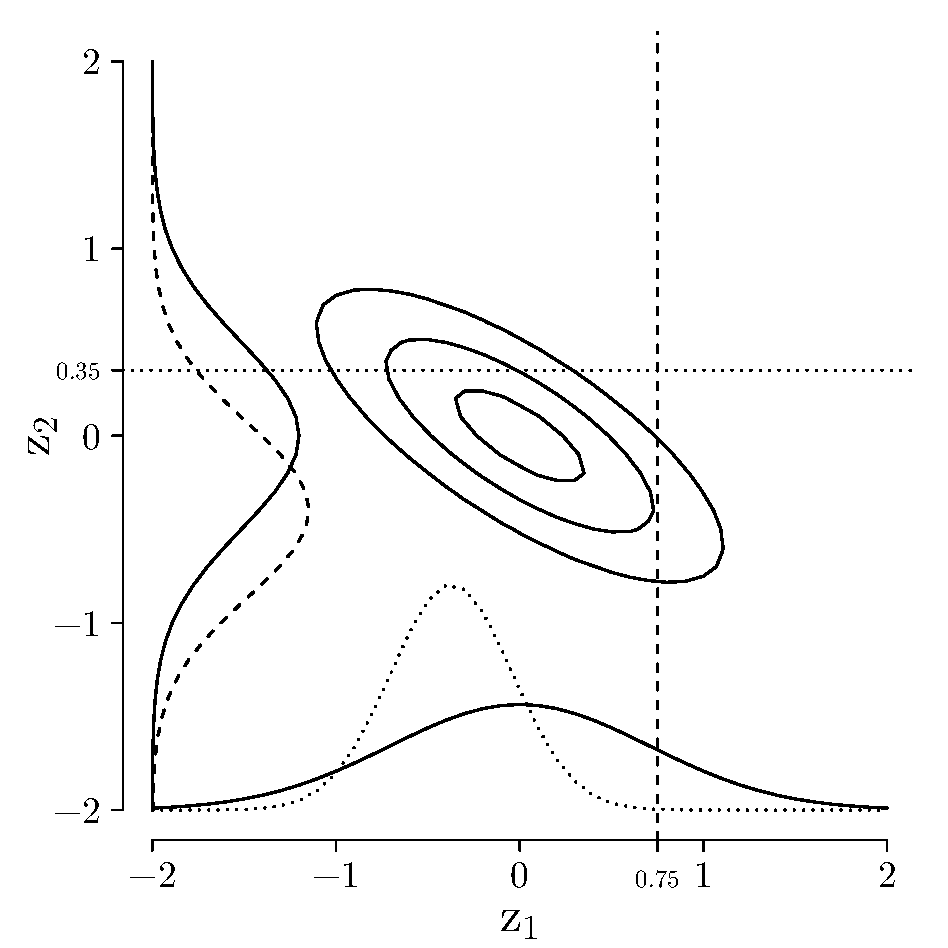
\includegraphics[scale=0.50]{../figures/chapter4/figures/plotBivariateNormal.pdf}
	\caption[Illustration of a bivariate Gaussian distribution]{An illustration of bivariate Gaussian distribution of random vector $Z = [Z_1, Z_2]$ having marginal means of $0.0$ and variances of $0.5$ and $0.25$, respectively and with covariance of $-0.265165$. The solid ellipsoids indicate the contour of joint density of random vector $[Z_1, Z_2]$. The two solid curves at the $x$- and $y$-axes indicate the marginal densities of $Z_1$ and $Z_2$, respectively. The dotted curve shows the conditional density of random variable $Z_1$ given $z_2 = 0.35$, while the dashed curve shows the conditional density of $Z_2$ given $z_1 = 0.75$.}
	\label{fig:plot_bivariate_normal}
\end{figure}

The joint density for Gaussian random vector is given in Eq.~(\ref{eq:gaussian_joint_density}.
\marginpar{joint density, illustrated}
For the bivariate random variable in the example, the density can be shown as contour plot in Fig.~\ref{fig:plot_bivariate_normal}.
In the figure, the solid ellipsoids are the iso-contours of the distribution, where each pair of values lies along the contour line has the same probability density value.

The two marginal densities for the example are shown as the solid curves plotted in the $x$ and $y$-axes, respectively.
\marginpar{marginal density, illustrated}
As illustrated, the marginalization of the joint distribution can be thought as a \emph{projection} of the $2$-dimensional distribution into each of the corresponding dimension.

Finally, two conditional distributions $p(z_1|z_2=0.35)$ and $p(z_2|z_1=0.75)$ are given as examples of conditioning a probability distribution in Fig.~\ref{fig:plot_bivariate_normal}.
\marginpar{conditional density, illustrated}
They are shown as dotted and dashed curves plotted in both axes.
Instead of projection to either of the axes, conditioning can be thought of as \emph{slicing} the $2$-dimensional distribution.
Conditioning two correlated random variables on one, in general, changes the shape of the distribution of the other variable.
From the figure, conditioning shifts the mean and reduces the variance of the resulting conditional distribution. 

% Drawing from Multivariate Gaussian
There are multiple ways to draw samples from a multivariate Gaussian distribution.
One method is particular require the deco
This method, so-called \emph{Cholesky} method, is detailed in Appendix.
A random number generator for the standard univariate distribution itself is widely available in many standard numerical computing environments.
The method in Appendix is used to generate 250 samples for the bivariate.
The resulting scatter plot and sample histograms of the marginal distributions 

% From Multivariate to Infinite Variate
\gls[hyper=false]{gp} can often be thought simply as a generalization of finite multivariate Gaussian random variable into an infinite multivariate one.
\marginpar{An entry to Gaussian Process}
To illustrate this idea, the marginal and conditional distributions of the bivariate distribution depicted in Fig.~ is plotted with the random variables at the same axis ($x$) while the range pf values of the variables are plotted in another axis ($y$).
The left panels shows the marginal distributions of random variables $Z_1$ and $Z_2$, where in Fig.~ they are plotted as black curves in their respective axes.
The center panel shows an observed value of $z_1 = 0.75$ depicted in Fig.~ as vertical dashed line.
Finally the right panel shows the conditional distribution of the non-observed variable $Z_2$ given $z_1 = 0.75$, which in Fig.~ was depicted as the dashed curve in the $y$-axis.
As it can be seen, the mean and standard deviation of the conditional distribution of $Z_2$ have been shifted and reduced, respectively, according to the information about $Z_1$.

Depiction in Fig.~ can easily be extended to a larger number of random variables, provided a valid mean vector and a valid covariance matrix.
Fig.~ shows such an extension to $15$-variate Gaussian random variable.
The origin of the underlying $15 \times 15$ covariance matrix is at the moment unimportant, but what the matrix does is defining how the variables are correlated to each other.
The whole covariance matrix, except its diagonal elements, is irrelevant in describing the marginal (Fig, left),
but it is significant in describing the shape of the conditional (Fig, right) according to Eqs.~.
As before, the conditional probability of the non-observed random variables are shifted and their standard deviation are reduced due to the information provided from the observed variables.

% Closing Sentence
Gaussian stochastic generalizes this procedure beyond $2$- or $15$-variate Gaussian random variable to an arbitrary number of variables at arbitrary locations in the real line.
It is easy to imagine that the shape of both marginals and conditionals will become smoother and smoother with increasing number of random variables in the $x$-axis, thus resembling more of a smooth function.
In fact, it is one of the interpretations of Gaussian process: a distribution over functions (citation). 

\subsection{Gaussian Process}

% What is a stochastic process
Gaussian stochastic process is a particular class of \emph{stochastic} or \emph{random process}.
\marginpar{Stochastic process}
Stochastic process is a collection of random variables, each of which are often indexed with certain underlying rules or ordering.
To be precise, a stochastic process is a set of random variables $\mathbf{Y} = \{Y_i, i \in I\}$, where $I$ is an index set, 
and it is defined on a probability space $(\Omega, \mathcal{F}, \mathbb{P})$, 
where $\Omega$, $\mathcal{F}$, and $\mathbb{P}$ are the sample space, the set of events, and the assigned probability to the event, respectively \cite{Syski2014}.

% Examples of stochastic process applications
For example, a time series can be modeled using stochastic process where the random variables are the observations taken at different time ordered sequentially.
\marginpar{Stochastic process applications}
In this case the index set is the time index of the observations.
A spatial model, as another example, can be modeled as a collection of random variables indexed by their locations in space.
And finally, in the metamodeling application, the random variables are collection of computational model output values at different input values.

% Gaussian stochastic process
\emph{Gaussian stochastic process} (GP, or Gaussian Random Field GRF) is defined as a collection of random variables, 
\emph{arbitrary number of which is a multivariate Gaussian random variable} \cite{Rasmussen2006, Debicki2014}.
\marginpar{Gaussian process}
To establish the connection with the notion of \emph{random function}, the collection of the above random variables refers to the collection of values of a random function $Y(\circ)$ at various possible input $\mathbf{x}$ in the domain $\mathcal{X} \subseteq \mathbb{R}^D$.
Specifically, $Y(\mathbf{x}), \, \text{for} \, \mathbf{x} \in \mathcal{X} \subseteq \mathbb{R}^D$ is a \emph{Gaussian process} if and only if for any choice from the finite set of input $\{\mathbf{x}_1, \mathbf{x}_2, \cdots, \mathbf{x}_L ; \, L \geq 1\}$, the random vector $\left[Y(\mathbf{x}_1), Y(\mathbf{x}_2), \cdots, Y(\mathbf{x}_L)\right]$ is a multivariate Gaussian random variable \cite{Santner2003}.

% Basic notation
A \gls[hyper=false]{gp} is fully specified by its mean and covariance functions, instead mean vector and covariance matrix.
A \gls[hyper=false]{gp} $Y$ on $\mathcal{X} \subseteq \mathbb{R}^D$ with a given mean function $m$ and covariance $K$ is denoted as
\begin{equation}
	Y(\mathbf{x}) \sim \mathcal{GP} \left(m(\mathbf{x}), K(\mathbf{x}, \mathbf{x}^*) \right)
\label{eq:gp_notation}
\end{equation}

% Mean Function
The mean function of a Gaussian process $Y(\mathbf{x})$ is the function $m: \chi \subseteq \mathbb{R}^D \mapsto \mathbb{R}$ defined as,
\marginpar{Mean function}
\begin{equation}
	m(\mathbf{x}) = \mathbb{E}[Y(\mathbf{x})]
\label{eq:gp_mean_functions}
\end{equation}

% Covariance Function
The covariance function of a Gaussian process $Y(\mathbf{x})$, on the other hand, is the function $K: (\chi \subseteq \mathbb{R}^D) \times (\chi \subseteq \mathbb{R}^D) \mapsto \mathbb{R}$ defined as,
\marginpar{Covariance Function}
\begin{equation}
	K(\mathbf{x}_i, \mathbf{x}_j) = \text{Cov}[Y(\mathbf{x}_i), Y(\mathbf{x}_j)]
\label{eq:gp_cov_functions}
\end{equation}
Notice that while the covariance function describes the covariance describes the covariance between pair of random function values, 
it is defined only as a function of the two inputs differentiating them.
Covariance function is also sometimes referred to as the \emph{covariance kernel} function as it defines the elements of the covariance matrix (see example below).
As such, not all functions of the pair of inputs $\mathbf{x}_i, \mathbf{x}_j$ are a \emph{valid} covariance function, but only the ones that yield a valid variance-covariance matrix given by condition in Eq.~(\ref{eq:covariance_matrix}). 

% Process Variance
Finally, the process variance is defined as the covariance between two random function values at the same input,
\marginpar{Process variance}
\begin{equation}
	K(\mathbf{x}_i, \mathbf{x}_i) = \text{Cov}[Y(\mathbf{x}_i), Y(\mathbf{x}_i)] = \mathbf{V}[Y(\mathbf{x}_i)]
\label{eq:process_variance}
\end{equation}

% Gaussian Stochastic Process and Multivariate Gaussian Random Variable
For a given finite $L$, a \gls[hyper=false]{gp} is reduced to a multivariate Gaussian random variable characterized by its mean vector $\boldsymbol{\mu}$ and covariance matrix $\boldsymbol{\Sigma}$,
\begin{equation}
	\begin{split}
		& [Y(\mathbf{x}_i)] \sim \mathcal{N}(\boldsymbol{\mu}, \boldsymbol{\Sigma}) \quad ; \, i = 1, 2, \cdots, L \\
		& \boldsymbol{\mu} = [m(\mathbf{x}_1), m(\mathbf{x}_2), \cdots, (\mathbf{x}_L)]^T \\
		  & \boldsymbol{\Sigma} = 
				\begin{pmatrix}
					\mathbf{V}[Y(\mathbf{x}_1)]  & \cdots & \text{Cov}[Y(\mathbf{x}_1), Y(\mathbf{x}_L)]\\
					\vdots	& \ddots & \vdots\\
					\text{Cov}[Y(\mathbf{x}_L), Y(\mathbf{x}_1)]  & \cdots  & \mathbf{V}[Y(\mathbf{x}_L)]\\
			\end{pmatrix} \\
	\end{split}
\label{eq:gp_to_mvn}
\end{equation}

% Example, introduced
The shape of the random function drawn from a \gls[hyper=false]{gp} is characterized by its mean and covariance functions.
Brief explanations of these functions will be provided in the next two subsections.
\marginpar{fully specified GP, an example}
In the meantime, an example of a fully specified Gaussian process will be used to illustrate how samples of functions can be drawn from such a stochastic process.
For the example, the following mean and covariance function will be used
\begin{equation}
	\begin{split}
		m(\mathbf{x}) & = 0 \\
		K(\mathbf{x}, \mathbf{x}^*) & = \sigma^2 \exp{\left[-\frac{(\mathbf{x} - \mathbf{x}^*)^2}{2\theta^2}\right]} = 10 \exp{\left[-\frac{(\mathbf{x} - \mathbf{x}^*)^2}{0.98}\right]}
	\end{split}
\label{eq:gp_example}
\end{equation}
where $x$ is a $1$-dimensional input parameter such that $x \in [-2, 2]$.
The mean function is set to constant zero, while the covariance function is chosen to be the so-called \emph{Gaussian covariance function} (which will be detailed in the sequel).
The Gaussian covariance function is parameterized by the characteristic length scale $\theta$ which is set to $0.70$.
This parameter is often referred to as the \emph{hyper-parameter} of the function.
Finally, $\sigma^2$ is the common variance of the stochastic process and it is set to $10$.

% Example continued, sample path
To generate random draws of function from the fully specified \gls[hyper=false]{gp} given in Eq.~(\ref{eq:gp_example}), 
first it must be specified at which input $x$ the function values are to be drawn.
\marginpar{sample path (trajectory) of a GP}
For the present example, $x$ is chosen to be uniformly distributed $\{-2 + 0.2 \times i\}_{i=0}^{20}$.
By specifying these locations, the $21$-variates Gaussian random variable can be constructed using Eq.~(\ref{eq:gp_to_mvn}) with the elements of variance-covariance matrix computed by the formula in Eq.~(\ref{eq:gp_example}) for all pairs of inputs.
Examples of $5$ realizations from the \gls[hyper=false]{gp} are shown in the left panel Fig~\ref{fig:sample_path_unconditional}.
A realization of a \gls[hyper=false]{gp} on a select input locations is also called a \emph{trajectory} or a \emph{sample path} of the process \cite{Santner2003}.
In this thesis the term \emph{sample path} will be used interchangeable with the term realization of a \gls[hyper=false]{gp}.
\normdoublefigure[pos=tbhp,
                  mainlabel={fig:sample_paths},
                  maincaption={Five realizations (sample paths) of a Gaussian process specified in Eq.~(\ref{eq:gp_example}) at $x_i = \{-2 + 0.2 \times i\}_{i=0}^{20}$. Shaded area indicates the area enveloped by twice standard deviation of the process (or $95\%$ probability region). In the right panel, the sample paths are drawn conditional on $6$ observed values (cross symbols).},%
                  leftopt={width=0.45\textwidth},%width=0.45\textwidth},
                  leftlabel={fig:sample_path_unconditional},
                  leftcaption={Unconditional},
                  %leftshortcaption={},%
                  rightopt={width=0.45\textwidth},%width=0.45\textwidth},
                  rightlabel={fig:sample_path_conditional},
                  rightcaption={Conditional},
                  %rightshortcaption={},
                  %spacing={\hfill}
                 ]
{../figures/chapter4/figures/plotSamplePath.pdf}
{../figures/chapter4/figures/plotSamplePathCond.pdf}

% Example, conditional simulation
Suppose now that values of $6$ variables are fully observed as follows $\{(x_i, y_i)\}_{i=1}^{6} = \{(-2.0, -0.75), (-1.2, 1.5), (-0.8, 2.75), (0.4, 3.75),$ 
$(1.2, -1.3), (1.8, -3.8)\}$.
\marginpar{conditional sample path}
The conditional $15$-variates Gaussian distribution can be constructed in the same manner as before with the conditional mean and covariance following Eqs.~.
Examples of $5$ sample paths from such conditional distribution are shown in Fig.~\ref{fig:sample_path_conditional}.
Observe that the standard deviations of the observed variables are zero and the areas between known values are substantially reduced.

% Strongly Stationary
An assumption for a class of stochastic process commonly made for convenience is \emph{stationarity}.
\marginpar{strongly stationary process}
A stochastic process $Y(\circ)$ is called \emph{strictly/strongly stationary} if and only if for any finite set of inputs $\{\mathbf{x}_1, \mathbf{x}_2,$
$\cdots, \mathbf{x}_L\} \in \mathcal{X} \subseteq \mathbb{R}^D$ with $L \leq 1$, 
and for $\mathbf{h} \in \mathbb{R}^D$ such that $\{(\mathbf{x}_1 + \mathbf{h}),$ 
$(\mathbf{x}_2 + \mathbf{h}), \cdots, (\mathbf{x}_L + \mathbf{h})\} \in \mathcal{X}$, the distribution of random vector $[Y(\mathbf{x}_1 + \mathbf{h}), $
$Y(\mathbf{x}_2 + \mathbf{h}), \cdots, Y(\mathbf{x}_L + \mathbf{h})]$ is \emph{the same as} the distribution of random vector $[Y(\mathbf{x}_1 + \mathbf{h}), Y(\mathbf{x}_2 + \mathbf{h}), \cdots, Y(\mathbf{x}_L + \mathbf{h})]$ \cite{Santner2003, Bachoc2013}.
In other words, the process is invariant under translation.

% Weakly Stationary
The \emph{weakly stationary process} used stronger assumption than the strongly stationary process.
\marginpar{weakly stationary process}
A stochastic process $Y(\circ)$ is called \emph{weakly stationary} if and only if
the first two moments of the process are constant.
As such, the weakly stationary process is also referred to as \emph{second-order stationary process}.

% Stationary, Isotropic Covariance Function
As mentioned, a \gls[hyper=false]{gp} is fully defined by its mean and covariance functions.
\marginpar{stationary, isotropic covariance function}
Therefore, if two \glspl[hyper=false]{gp} have the same mean and covariance functions defined over the same domain then the two process have exactly the same same distribution and are the same process.
Furthermore, for the case of \gls[hyper=false]{gp}, the notions of strongly stationary and weakly stationary coincide.
This implies that a stationary \gls[hyper=false]{gp} has a constant mean and a constant variance, as well as a covariance function that satisfies the condition of being invariant under translation as follows,
\begin{equation}
	\text{Cov}[Y(\mathbf{x}_i), Y(\mathbf{x}_j)] = \text{Cov}[Y(\mathbf{x}_i + \mathbf{h}), Y(\mathbf{x}_j + \mathbf{h})] = K (\mathbf{x}_i - \mathbf{x}_j)
\label{eq:stationary_covariance}
\end{equation}
In stationary \gls[hyper=false]{gp}, the covariance of random function values between two input points is only determined by the \emph{distance} between the two inputs and the covariance function is called \emph{stationary, isotropic covariance function} \cite{Rasmussen2006}. 
The notion of distance used in the above definition depends on the specific type of the covariance function as will be explained in the next subsection.
Additionally, following Eq.~\ref{eq:stationary_covariance}, the process variance can be defined as the covariance at zero distance or $K(0)$, which is constant across input parameter space.

% Non-Stationary Gaussian Process
A more flexible class of \gls[hyper=false]{gp} models can be constructed by relaxing the stationarity assumption.
\marginpar{non-stationary process}
However, stationarity is often assumed because it requires less assumption than the alternatives, considered non-informative, and therefore more generic \cite{Currin1991}.
Moreover, the stationary process remains important to study as they serve as building block for more advanced models \cite{Santner2003}.
For instance, the stationarity assumption can be relaxed simply by considering non-constant mean function as proposed in  \cite{Marrel2008,Ginsbourger2009}, while keeping the covariance part stationary.
Another alternative is to consider multiple stationary covariance functions defined for each partitioned region of the whole input parameter space as proposed in \cite{Gramacy2008}.

\subsection{Covariance Kernel Function}\label{sub:gp_covariance}

Covariance kernel function determines the covariation structure of dependent data.
This, in turn, determines the behavior (or shape) of the sample path of the outputs between input points.
For a stationary covariance function, it is more convenient to separate the constant stochastic process variance $\sigma^2$ and the stochastic process kernel correlation function $R(\circ,\circ)$ between two input points using the following relation,
\begin{equation}
	K (\mathbf{x}_i, \mathbf{x}_j) = \sigma^2 R(\mathbf{x}_i, \mathbf{x}_j) 
	\label{eq:cov_function}
\end{equation}
where $R$, the correlation kernel function, is defined such that $\forall \, \mathbf{x}_i, \mathbf{x}_j \in \chi \subseteq \mathbb{R}^D$;
and $\sigma^2$ is the aforementioned stochastic process variance, which determines the scale of variation magnitude of the output space.

In the following, three different types of stationary correlation kernel functions are presented. 
These functions, namely \emph{Gaussian}, \emph{power-exponential}, and \emph{Mat\'ern class} kernels are widely applied in the simulation metamodeling literature.
\marginpar{one-dimensional correlation kernel, $r$}
For each, the function is defined and several sample paths are drawn to illustrate the effect of different kernels and different respective parameters on the realization.
At first, only $1$-dimensional kernel functions denoted by $r(x_i, x_j)$ are described.
Afterward, these $1$-dimensional functions are used to create a multidimensional kernel function $R(\mathbf{x}_i, \mathbf{x}_j)$ by means of tensor product.

\subsubsection{Gaussian Kernel}\label{subsub:gp_gaussian_cov}

The Gaussian correlation kernel function, also known as the \emph{squared exponential} kernel, is given by the following formula \cite{Roustant2012,Santner2003,Rasmussen2006},
\begin{equation}
	r(x_i, x_j; \theta) = \exp{\left[- \frac{(x_i - x_j)^2}{2 \theta^2}\right]}
\label{eq:gaussian_kernel}
\end{equation}

The Gaussian kernel is parameterized by only a single \emph{hyper-parameter} $\theta$ that defines the characteristic length-scale of the process (or simply \emph{the scale parameter}).
\marginpar{characteristic length-scale parameter}
Fig.~\ref{fig:plot_corrfun_gauss} shows the correlation value as function of Euclidian distance, $(x_i - x_j)^2$, between input points according to the Gaussian kernel, 
for 3 different characteristic length scales.
Obviously, for smaller $\theta$ the correlation between two inputs drops more quickly over shorter distance, and vice versa.
\begin{figure}[bth]
	\centering
	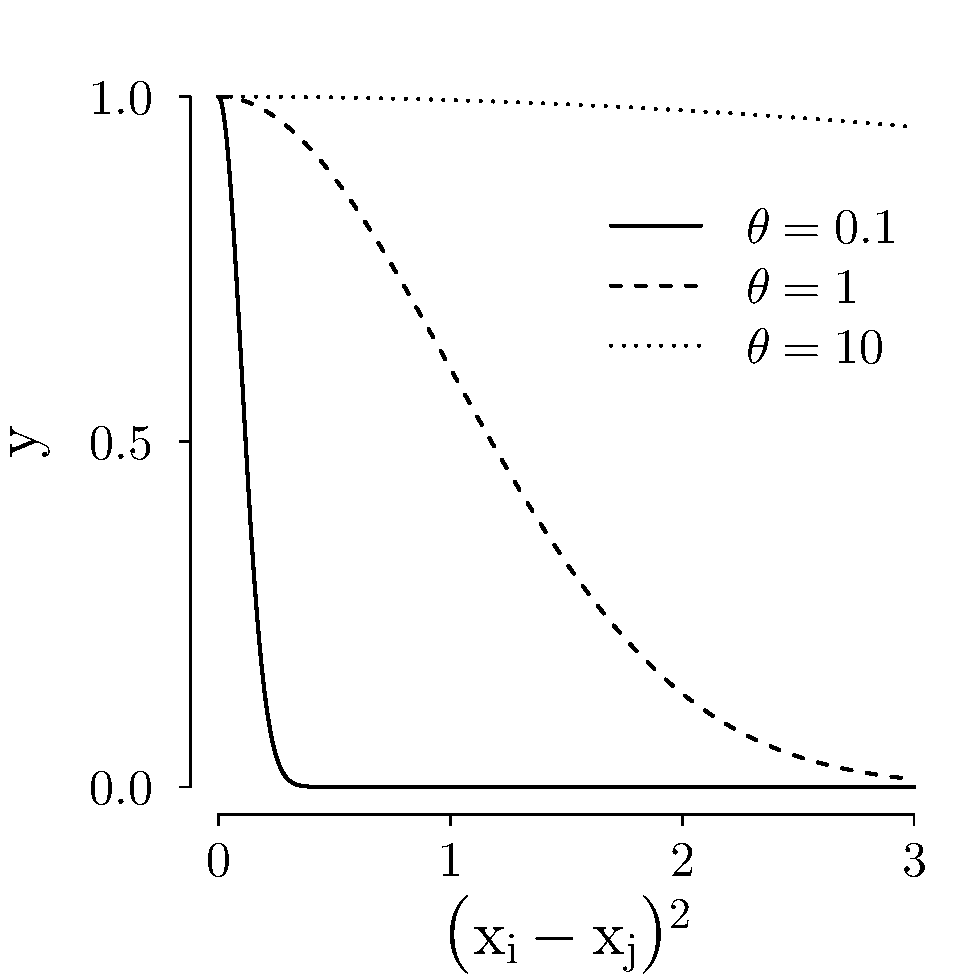
\includegraphics[scale=0.35]{../figures/chapter4/figures/plotCorrFunGauss.pdf}
	\caption[Gaussian correlation kernels with 3 different characteristic length scales]{Examples of Gaussian correlation kernels with 3 different characteristic length scales}
	\label{fig:plot_corrfun_gauss}
\end{figure}

The characteristic length-scale of a Gaussian kernel determines the range over which the distance between two input locations affects the output correlation.
To be precise, the notion how similar (or dissimilar) two input locations is defined relative to the characteristic length-scale.
With a very short length-scale, the output of random functions becomes easily uncorrelated except for a very close (similar) inputs.
The realization of the process, therefore, will exhibit more erratic behavior in short length scale as it allows for more abrupt changes over shorter distance and less dependent of the neighboring values.
On the other hand, with a longer length-scale, the output of random function tends to be highly correlated except for very different input values and thus the realization will exhibit more rigid pattern.
Gaussian kernel, however, always produces smooth realization. That is, two input points that have a zero separation on the limit are both continuous and differentiable 
(see the neighborhood of the origin of Fig.~\ref{fig:plot_corrfun_gauss}).
The Gaussian kernel is widely applied in the metamodeling literature and almost become a default choice for the correlation kernel \cite{Kennedy2006},
though as mentioned in \cite{Rasmussen2006} the overly smooth process can result in either physically unrealistic or numerically difficult situations (i.e., the resulting variance-covariance matrix is ill-conditioned for poorly select design points).

Fig.~\ref{fig:plot_corrfun_gauss_realizations} shows a comparison between realizations of a \gls[hyper=false]{gp} using Gaussian kernel for three different characteristic length-scales.
The short length scale, illustrated on the left panel, allows for more sudden change in the output values while the long length scale on the right shows smoother (and rigid) pattern for the same input domain ($0.0 \leq x \leq 3.0$). 
Also notice that the realizations with the shorter length scale produces more local maxima and minima.
\bigtriplefigure[pos=tbhp,
								 mainlabel={fig:plot_corrfun_gauss_realizations},
			           maincaption={Examples of realizations from \gls[hyper=false]{gp} with Gaussian correlation kernel for $3$ different values of characteristic length-scale. The plotting range of the $y$-axis for each panel are set to $\pm \, 3 \times \sigma$. Each process has the same process variance, $\sigma^2 = 1.0$},
			           mainshortcaption={Realizations of random function drawn from \gls[hyper=false]{gp} with Gaussian kernel},%
			           leftopt={width=0.30\textwidth},
			           leftlabel={fig:plot_corrfun_gauss_realization_1},
			           leftcaption={},
			           midopt={width=0.30\textwidth},
			           midlabel={fig:plot_corrfun_gauss_realization_2},
			           midcaption={},
			           rightopt={width=0.30\textwidth},
			           rightlabel={fig:plot_corrfun_gauss_realization_3},
			           rightcaption={},
			           spacing={},
			           spacingtwo={}]
{../figures/chapter4/figures/plotCorrFunGaussRealization_1}
{../figures/chapter4/figures/plotCorrFunGaussRealization_2}
{../figures/chapter4/figures/plotCorrFunGaussRealization_3}

\subsubsection{Power-Exponential Kernel}

The Gaussian correlation kernel belongs to a wider class of $2$-parameter kernel function family called the \emph{power-exponential} kernel and is given by \cite{Roustant2012,Santner2003,Rasmussen2006},
\begin{equation}
	r(x_i, x_j; \theta, p) = \exp{\left[ - \left( \frac{|x_i - x_j|}{\theta} \right)^p \right]} \, \text{for} \, \theta > 0.0 \, \text{and} \, 0 < p \leq 2
\label{eq:powexp_kernel}
\end{equation}

The parameter $\theta$ remains the (length-) scale parameter of the process, while the additional parameter $p$ is referred to as the shape parameter of the process.
\marginpar{shape parameter}
Specifically, the shape parameter $p$ determines the differentiability of the process at the origin (citation needed).
Fig.~\ref{fig:plot_corrfun_powexp} shows the correlation value of power-exponential kernel with three different values of $p$ and $\theta$ as function of $L_1$ norm.
\bigtriplefigure[pos=tbhp,
								 mainlabel={fig:plot_corrfun_powexp},
			           maincaption={Examples of power exponential kernel functions for different values of shape parameter $p$ and scale parameter $\theta$ as function of $L_1$ norm.},
			           mainshortcaption={Examples of power exponential kernel functions},%
			           leftopt={width=0.30\textwidth},
			           leftlabel={fig:plot_corrfun_powexp_1},
			           leftcaption={},
			           midopt={width=0.30\textwidth},
			           midlabel={fig:plot_corrfun_powexp_2},
			           midcaption={},
			           rightopt={width=0.30\textwidth},
			           rightlabel={fig:plot_corrfun_powexp_3},
			           rightcaption={},
			           spacing={},
			           spacingtwo={}]
{../figures/chapter4/figures/plotCorrFunPowExp_1}
{../figures/chapter4/figures/plotCorrFunPowExp_2}
{../figures/chapter4/figures/plotCorrFunPowExp_3}

Although, strictly speaking, only when $p = 2$ that the power-exponential correlation is differentiable at the origin (thus guarantee the smoothness of the realization),
the shape parameter does dictate the apparent roughness of the sample path drawn from the process as illustrated in Fig.~\ref{fig:plot_corrfun_gauss_realizations} \cite{Rasmussen2006}.
\bigtriplefigure[pos=tbhp,
								 mainlabel={fig:plot_corrfun_powexp_realizations},
			           maincaption={Several realizations from \gls[hyper=false]{gp} with power-exponential kernel functions of different shape $p$ and scale $\theta$ parameters.},
			           mainshortcaption={Examples of power exponential kernel functions},%
			           leftopt={width=0.30\textwidth},
			           leftlabel={fig:plot_corrfun_powexp_realization_1},
			           leftcaption={},
			           midopt={width=0.30\textwidth},
			           midlabel={fig:plot_corrfun_powexp_realization_2},
			           midcaption={},
			           rightopt={width=0.30\textwidth},
			           rightlabel={fig:plot_corrfun_powexp_realization_3},
			           rightcaption={},
			           spacing={},
			           spacingtwo={}]
{../figures/chapter4/figures/plotCorrFunPowExpRealizations_1}
{../figures/chapter4/figures/plotCorrFunPowExpRealizations_2}
{../figures/chapter4/figures/plotCorrFunPowExpRealizations_3}

It is argued in \cite{Marrel2008} that the power-exponential kernel function is an appropriate choice in metamodeling application due to its flexibility of representing different shape with respective to its regularity and differentiability mainly controlled through the additional parameter $p$.
\marginpar{exponential kernel}
For instance, Gaussian correlation kernel is a special case of the power-exponential kernel when $p$ equals to 2. 
Another special case is when $p = 1$ which is called the \emph{exponential} kernel.
In this particular case, realizations of which are depicted in Fig.~\ref{fig:plot_corrfun_powexp_realization_2}, the process is continuous but not differentiable \cite{Rasmussen2006}.

\subsubsection{Mat\'ern Class Kernel}

The Mat\'ern class correlation kernel is another $2$-parameter kernel family and it is given by the following formula
\lipsum[2]

\subsection{Multidimensional Construction}

In order to create a valid multidimensional correlation kernel function from a valid $1$-dimensional correlation function given above, 
a tensor product construction is used as follows,
\marginpar{tensor product}
\begin{equation}
	R(\mathbf{x}_i, \mathbf{x}_j) = \prod_{d = 1}^{D} r_d \left(x_i^{(d)}, x_j^{(d)}\right)
\label{eq:tensor_product}
\end{equation}
where $r_d$ is a $1$-dimensional correlation kernel function for the $d$-th input dimension;
while $x_i^{(d)}$ and $x_j^{(d)}$ are a pair of values in the $d$-th input dimension.

Although it is possible to mix different types of correlation function or use different kind of multidimensional construction (see for example \cite{Higdon2002}),
the tensor product with the same correlation function for each input dimension is the most well-established 
and, by far, the most popular approach in the applied metamodeling literature to date \cite{Roustant2012,Sacks1989,Sacks1989a,Santner2003,Currin1991,Marrel2008,Bachoc2014,Kennedy2006,Jones2009}.

Fig.~\ref{fig:random_surfaces} shows two examples of realizations of random surface drawn from a multidimensional \gls[hyper=false]{gp} with the same process variance ($\sigma^2 = 10.0$) but with two different correlation kernels.
On the left is an example of a realization drawn from the \gls[hyper=false]{gp} using Gaussian correlation kernel function with relatively the characteristic length scale in $y$-direction is four times the scale in $x$-direction.
On the right is an example of a realization drawn from the \gls[hyper=false]{gp} using Mat\'ern correlation kernel function.
For this case, the shape parameter is three times larger in the $x$-direction than in the $y$-direction.
As such, for both cases, the surface appears less smooth in one of the direction.
\bigdoublefigure[pos=tbhp,
                 mainlabel={fig:random_surfaces},
								 mainshortcaption={Random surface realizations},
                 maincaption={Two random surfaces drawn from two different multidimensional \gls[hyper=false]{gp} with the same process variance of $\sigma^2 = 9.0$. Differences in the scale (for Gaussian) and shape (for Mat\'ern) parameters for the inputs yield smoother path in one direction. The color scheme is the same for both plots with the range of $\pm \, 3 \times \sigma$.},
                 leftopt={width=0.475\textwidth},
                 leftlabel={fig:random_surface_gaussian},
                 leftcaption={Gaussian, $\theta_x = 0.5, \theta_y = 2.0$},
                 rightopt={width=0.475\textwidth},
                 rightlabel={fig:random_surface_matern},
                 rightcaption={Mat\'ern, $\theta_x = 1.5, \theta_y = 0.5$},
                 ]
{../figures/chapter4/figures/plotRandomSurface_1}
{../figures/chapter4/figures/plotRandomSurface_2}

\subsection{Process Variance}

For stationary \gls[hyper=false]{gp}, the shape of sample path is determined solely by the form of the correlation.
The role of process variance according to Eq.~(\ref{eq:cov_function}) is to determine the scale of magnitude of output variation. 
Fig.~\ref{fig:plot_process_variance} gives an illustration of realizations drawn from a set of \glspl[hyper=false]{gp} with the same kernel correlation function (i.e., Gaussian kernel with $\theta = 1.0$), 
but with different values of process variance.
As it can be seen, the visible features of the realizations remain the very similar to each other.
What has changed, however, is the scale of the variation in the output space.  
\bigtriplefigure[pos=tbhp,
								 mainlabel={fig:plot_process_variance},
			           maincaption={Realizations of \gls[hyper=false]{gp} with Gaussian correlation kernel for $3$ different values of process variance. The plotting range of the $y$-axis for each panel are set to $\pm \, 3 \times \sigma$.},
			           mainshortcaption={Effect of different process variance values on GP realization},%
			           leftopt={width=0.30\textwidth},
			           leftlabel={fig:plot_process_variance_1},
			           leftcaption={},
			           midopt={width=0.30\textwidth},
			           midlabel={fig:plot_process_variance_2},
			           midcaption={},
			           rightopt={width=0.30\textwidth},
			           rightlabel={fig:plot_process_variance_3},
			           rightcaption={},
			           spacing={},
			           spacingtwo={}]
{../figures/chapter4/figures/plotProcessVariance_1}
{../figures/chapter4/figures/plotProcessVariance_2}
{../figures/chapter4/figures/plotProcessVariance_3}

\subsection{Mean Function}
%**************************************************************
\section{Gaussian Process Metamodel}\label{sec:gp_metamodeling}
%**************************************************************

% Kriging Model, Drift and Bias
To formalize the use of in the meta-modeling of computer simulation, 
consider once again a computer code represented as 

The output of code at an arbitrary inputs, $\mathbf{x_o}$, is then modeled using a predictor of the following form
\begin{equation}
	Y (\mathbf{x_o}) = \mu (\mathbf{x_o}) + Z (\mathbf{x_o})
\label{eq:kriging_model}
\end{equation}
The equation above, also known as the \emph{Kriging} model (cite Owen, Simpson, Dupuy)\footnote{in fact, the term Kriging model will be used interchangeably as Gaussian process metamodel in this thesis} , consists of two components:
\begin{itemize}
	\item The \emph{mean/drift/trend} term, a deterministic function
	\begin{equation}
		\mu: \mathbf{x} \in \mathcal{X} \subseteq \mathbb{R}^D \mapsto \mathbb{R}
	\label{eq:trend_function_mapping}
	\end{equation}
	The trend term, in turn, usually consists of general linear model of polynomials (cite Owen and Dupuy, Marrel).
	\begin{equation}
		\mu(\mathbf{x}) = \sum_{j=0}^{k} \beta_j h_j(\mathbf{x})
	\label{eq:trend_function_definition}
	\end{equation}
	The trend term captures the global input output space which has an equivalent interpretation to that of a linear regression model\footnote{$Y() = \mu(\mathbf{x} + \epsilon$ with $\epsilon$ is Normally independent and identically distributed measurement error term}.
	\item The \emph{bias} term, a stochastic process. 
	This term, in turn, usually modeled using zero mean, stationary Gaussian stochastic process (such as presented in Section~\ref{sub:gp_covariance}).
	\begin{equation}
		\mathcal{Z}(\mathbf{x}) \sim \mathcal{GP}(0, R(\mathbf{x},\mathbf{x}^*))
	\label{eq:stationary_gp}
	\end{equation}
	The bias term captures the local variation of the output space such that it pulls the predictor.
	The term local here is referring to the neighborhood of training data.
	In linear regression model the error between observation and prediction is due to experimental error.
	This, in essence, what distinguishes kriging model to ordinary least square.
	Furthermore, by using stationary Gaussian process it is also assumed that the bias term will be a function of distance between design points and test point. 
\end{itemize}

% Hyper-parameters
Additionally, according to the above formulation, a \gls[hyper=false]{gp} metamodel contains several parameters called the \emph{hyper-parameters}.
\marginpar{hyper-parameters}
This term is used to distinguish them from the parameter associated with the original simulation model which is referred to as the model parameter or often simply as the parameter.
The hyper-parameters of a \gls[hyper=false]{gp} metamodel are the ones associated with the chosen trend function (Eq.~\ref{eq:trend_function_definition});
the ones associated with select correlation functions (Section~\ref{sub:gp_covariance}); and the one associated with the process variance $\sigma^2$.
The total number of hyper-parameters depends on the number of simulation model parameters as well as the select structure of mean and correlation functions.
For instance, for a $D$-parameter simulation model represented using \gls[hyper=false]{gp} metamodel with a constant mean and Gaussian correlation functions (Eq.~(\ref{eq:gaussian_kernel})), 
the total number of hyper-parameters $\boldsymbol{\Psi} = (\mu, \sigma^2, \boldsymbol{\theta})$ is $D + 2$.
On the other hand, the same model represented using a \gls[hyper=false]{gp} metamodel with linear first-order mean and power-exponential functions (Eq.~(\ref{eq:powexp_kernel})),
the total number of the hyper-para\-meters $\boldsymbol{\Psi} = (\boldsymbol{\beta}, \sigma^2, \boldsymbol{\theta}, \mathbf{p})$ is $3D + 2$.

% Three classes of Kriging Model
Two classes of Kriging models can be distinguished depending on what is known about the hyper-parameters: 
\emph{Simple Kriging} and \emph{Universal Kriging}.

\subsection{Simple Kriging}\label{sub:gp_sk}

% Simple Kriging
Simple Kriging is the simplest case of the Kriging models where all the hyper-parameters involved are assumed to be known.
\marginpar{simple Kriging}
In that case the estimation of code output at an arbitrary input location becomes straightforward.
Following the formulation above, 
a \gls[hyper=false]{gp} metamodel, then by definition implies that the computer code outputs at every input locations are jointly Gaussian.
As such, the code outputs at the training inputs $\mathbf{DM} = \{\mathbf{x}_i\}_{i=1}^N, Y(\mathbf{DM}) = (Y(\mathbf{x}_1), Y(\mathbf{x}_2), \cdots, Y(\mathbf{x}_N))$
and the output at an arbitrary input $\mathbf{x}_o$, $Y(\mathbf{x}_o)$ are distributed jointly as an $N+1$-dimensional Gaussian,
\begin{equation}
	\begin{bmatrix}
			Y(\mathbf{DM}) \\
			Y(\mathbf{x}_o)
		\end{bmatrix} \sim \mathcal{N} \left(
			\begin{bmatrix}
				\mu(\mathbf{DM}) \\
				\mu(\mathbf{x}_o)
			\end{bmatrix}, \sigma^2
			\begin{bmatrix}
				R(\mathbf{DM}, \mathbf{DM})  & R(\mathbf{DM}, \mathbf{x}_o) \\
				R(\mathbf{x}_o, \mathbf{DM}) & R(\mathbf{x}_o, \mathbf{x}_o)
			\end{bmatrix} \right)
\label{eq:joint_training_test}
\end{equation}
where
\begin{itemize}
	\item $\mu(\mathbf{DM})$ is the vector of mean at the training points;
		\begin{equation}
			\mu(\mathbf{DM}) = (\mu(\mathbf{x}_1), \mu(\mathbf{x}_2), \cdots, \mu(\mathbf{x}_N)) 
		\label{eq:training_mean_vector}
		\end{equation}
	\item $\mu(\mathbf{x}_o)$ is the mean at an arbitrary test location;
	\item $R(\mathbf{DM}, \mathbf{DM})$ is the $N \times N$ correlation matrix between outputs at the training points
		\begin{equation}
			R(\mathbf{DM}, \mathbf{DM}) = 
				\begin{bmatrix}
					R(\mathbf{x}_1, \mathbf{x}_1) & \cdots												& R(\mathbf{x}_1, \mathbf{x}_N) \\
					\vdots												& \ddots												&	\vdots \\
					R(\mathbf{x}_N, \mathbf{x}_1)	&	R(\mathbf{x}_N, \mathbf{x}_2) & R(\mathbf{x}_N, \mathbf{x}_N)
				\end{bmatrix}
		\label{eq:training_correlation_matrix}
		\end{equation}
	\item $R(\mathbf{DM}, \mathbf{x}_o) = R(\mathbf{x}_o, \mathbf{DM})$ is the $N \times 1$ vector of correlation between outputs at the training points and the output at the test point
			\begin{equation}
				R(\mathbf{x}_o, \mathbf{DM}) = R(\mathbf{DM}, \mathbf{x}_o) =  
					\begin{bmatrix}
						R(\mathbf{x}_o, \mathbf{x}_1) \\
						\vdots												\\
						R(\mathbf{x}_o, \mathbf{x}_N)	
					\end{bmatrix}
			\label{eq:training_test_correlation}
			\end{equation}
		\item and $R(\mathbf{x}_o, \mathbf{x}_o)$ is the correlation of the output at the test input with itself. By definition this correlation is equal to $1$.
\end{itemize}

% Conditional Distribution, Simple Kriging
Provided that the outputs at the training inputs are fully observed (i.e., the code is actually run at those inputs),
then the output at the test input $Y(\mathbf{x}_o)$ \emph{given	} the observed outputs $Y(\mathbf{DM}) = \mathbf{y} = (y_1, y_2, \cdots,$ 
$y_N)^T$ is a conditional Gaussian random variable,
\begin{equation}
	Y(\mathbf{x}_o) | Y(\mathbf{DM}) = \{y_i\}_{i=1}^N \sim \mathcal{N} \left( m_{SK}(\mathbf{x}_o), s^2_{SK}(\mathbf{x})\right)
\label{eq:joint_training_test}
\end{equation}
where $\mu_{SK}$ and $s^2_{SK}$ are the mean and the variance of the distribution, respectively.
They are also often referred to as the \emph{simple Kriging mean} and \emph{simple Kriging variance}, respectively.

% Kriging Predictor, the mean
The simple Kriging mean (or the \emph{Kriging predictor}) is expressed as follow
\marginpar{(simple) Kriging mean}
\begin{equation}
	m_{SK} (\mathbf{x}_o) = \mu (\mathbf{x}_o) + R^T(\mathbf{x}_o, \mathbf{DM}) R^{-1}(\mathbf{DM}, \mathbf{DM}) (\mathbf{y} - \mu(\mathbf{DM}))
\label{eq:mean_sk}
\end{equation}
% Kriging Variance
The simple Kriging variance, on the other hand, is expressed as
\marginpar{(simple) Kriging variance}
\begin{equation}
	s^2_{SK} (\mathbf{x}_o) = \sigma^2 (1 - R^T(\mathbf{x}_o, \mathbf{DM}) R^T(\mathbf{DM}, \mathbf{DM}) R(\mathbf{x}_o, \mathbf{DM}))
\label{eq:variance_sk}
\end{equation}
The expressions for the mean and the variance above are obtained through the conditioning operation of the Gaussian random vector in Eq.(~\ref{eq:joint_training_test}) (See Appendix). 
In practice, the Kriging mean are used as a predictor of the code output at an arbitrary input location, 
while the variance is used as a measure of error of that prediction.

% Interesting Observation
The simple Kriging model has several interesting features:
\begin{itemize}
	% Linearity
	\item The Kriging predictor given by the mean in Eq.(\ref{eq:mean_sk}) is a \emph{linear predictor}. 
				\marginpar{linear predictor}
	      In other words, the centered predictor ($m_{SK}(\mathbf{x}_o) - \mu (\mathbf{x}_o)$)  is a weighted linear combination of the centered data 
	      ($\mathbf{y} - \mu(\mathbf{DM})$).
				The weights depends on the correlation function $R(\circ,\circ)$, the design of training points $\mathbf{DM}$, and the distance between the test point and the training points.
	% Interpolant
	\item The variance collapses at the training points, that is plugging-in $\mathbf{x}_i \in DM$ into Eq.(\ref{eq:variance_sk}) will yield $s^2_{SK}(\mathbf{x}_i) = 0$.
				\marginpar{Kriging as an interpolant}
	      As such, the Kriging predictor is also an \emph{interpolant}, which exactly fits the observed data (i.e., deterministic code output at the training inputs).
	% Dependence of the variance
	\item The variance on a given test point does not depend on the observed data.
				\marginpar{Variance as function of distance between test and training points}
	      Strictly speaking, it is only dependent on the process variance $\sigma^2$ and the correlation function $R(\circ,\circ)$.
				Furthermore, the variance on a given test point is also equal or less than the process variance, 
				the difference of which depends on the distance between $\mathbf{x}_o$ and the training points $\mathbf{DM}$.
				The closer $\mathbf{x}_o$ is to the training points, the smaller the variance at that point.
	% Epistemic Uncertainty interpretation
	\item Being the variance of a conditional Gaussian distribution, the Kriging variance can be intuitively interpreted as the posterior \emph{uncertainty} of the prediction given the observed data.
				\marginpar{Variance as measure of epistemic uncertainty}
	      The nature of this uncertainty is epistemic as, in the case of this thesis, the computer code that underlies the observed data is deterministic.
				In other words, the uncertainty associated with the prediction at an arbitrary input is due to the lack of knowledge because the code itself is not run at that point.
				However, the prediction at that point is informed by the observed data as contained in the training data.
\end{itemize}

\subsection{Universal Kriging and Hyper-Parameter Estimation}\label{sub:gp_uk}

% Ordinary and Universal Kriging
In most practical situation, however, the values of the hyper-parameters are not known a priori.
This is indeed the case for the Universal Kriging model where all the hyper-parameters values associated with both a linear mean and covariance functions are to be estimated simultaneously from the training data.


% Likelihood
To estimate the values of the hyper-parameters $\boldsymbol{\Psi}$ of a chosen structure of mean and covariance functions,
\marginpar{the likelihood function} 
it is should be first acknowledged that under \gls[hyper=false]{gp} model, the distribution of the observed data given a Gaussian process $\mathbf{y} \, | \, Y(\mathbf{x}), \boldsymbol{\Psi}$ is Gaussian such that
\begin{equation}
	\mathcal{L}(\boldsymbol{\Psi}; \mathbf{y}) = \frac{1}{(2\pi)^{N/2}(\sigma)^{N/2}|\mathbf{R}|^{1/2}} \exp{\left[- \frac{(\mathbf{y} - \mathbf{F} \boldsymbol{\beta})^T \mathbf{R}^{-1} (\mathbf{y} - \mathbf{F} \boldsymbol{\beta})}{2\sigma^2}\right]}
\label{eq:gp_likelihood}
\end{equation}
The term above is called the \emph{likelihood} function.
The slight change of perspective from a conditional density function to a common function is due to the fact that the data is already observed (cite Bayesian Tutorial).
For compactness, the $N \times N$ correlation matrix between outputs at the training points $R(\mathbf{DM}, \mathbf{DM})$ are written simply as $\mathbf{R}$;
and the $N \times M$ basis function matrix at the training points $\mathbf{f}(\mathbf{DM})$ as $\mathbf{F}$.
Finally, it is also implied in the formulation that the chosen \gls[hyper=false]{gp} is fully specified through its hyper-parameterization $\boldsymbol{\Psi}$ on $\boldsymbol{\mu}$ and $\mathbf{R}$
such that the notation $Y(\mathbf{x})$ is removed from the expression.

% Maximum Likelihood Estimation / Empirical Bayes, Profile/Concentrated Likelihood
Starting from the likelihood formulation, a common approach to estimate the hyper-parameters values is by selecting the ones that maximize the likelihood for a given observed data $\mathbf{y}$.
\marginpar{maximum likelihood estimation / empirical Bayes}
This estimation procedure, the maximum likelihood estimation, is also known in the literature as the \emph{empirical Bayes} (citation needed, Bayarri, Arendt) where the estimation is derived strictly from available data.
The procedures is as follow:
First, the hyper-parameters related to $\mathbf{R}$, $\boldsymbol{\Theta} = \{\boldsymbol{\theta}, \mathbf{p}\}$, are initially assumed to be known to estimate $\sigma^2$ and $\boldsymbol{\beta}$ by minimizing the negative log likelihood\footnote{logarithm is often taken on the likelihood to avoid underflow error when dealing with a very small number} (which is equivalent to maximizing the likelihood),
\begin{equation}
	\hat{\boldsymbol{\beta}}, \hat{\sigma}^2; \boldsymbol{\Theta} = \underset{\boldsymbol{\beta},\sigma^2}{\arg\min} - \ln \mathcal{L} (\hat{\boldsymbol{\beta}}, \hat{\sigma}^2 ; \hat{\boldsymbol{\Theta}})
\label{eq:concentrated_likelihood_1}
\end{equation} 
yielding
\begin{equation}
	\begin{split}
		\hat{\boldsymbol{\beta}} & = (\mathbf{F} \mathbf{R}_{\boldsymbol{\Theta}}^{-1} \mathbf{F})^{-1} \mathbf{F}^T \mathbf{R}_{\boldsymbol{\Theta}}^{-1} \mathbf{y} \\
		\hat{\sigma}^2           & = \frac{(\mathbf{y} - \mathbf{F} \hat{\boldsymbol{\beta}})^T \mathbf{R}_{\boldsymbol{\Theta}}^{-1} (\mathbf{y} - \mathbf{F} \hat{\boldsymbol{\beta}})}{N}\\
	\end{split}
\label{eq:beta_sigma_ml}
\end{equation}
The estimated $\hat{\boldsymbol{\beta}}$ and $\hat{\sigma}^2$ are then fed back to Eq.~(\ref{eq:gp_likelihood}) to obtain the so-called \emph{concentrated/profile likelihood} (citation needed).
\marginpar{concentrated (profile) likelihood}
The term is due to the fact that the full likelihood has been further conditioned by setting some of the parameters 
(in this case, $\boldsymbol{\beta}$ and $\sigma^2$) to constants (in this case, their maximum likelihood estimates).
This procedure eases the numerical difficulty of finding simultaneously the maximum likelihood estimates of all the hyper-parameters in high-dimensional space (citation needed).
Finally, the estimate of $\hat{\boldsymbol{\Theta}}$ is obtained through its the maximum likelihood
\begin{equation}
	\hat{\boldsymbol{\Theta}} ; \hat{\boldsymbol{\beta}}, \hat{\sigma}^2 = \underset{\boldsymbol{\Theta}}{\arg\min} - \ln \mathcal{L} (\hat{\boldsymbol{\Theta}};\hat{\boldsymbol{\beta}}, \hat{\sigma}^2)
\label{eq:theta_ml}
\end{equation}
The computation of Eq.~\ref{eq:theta_ml} is then carried out using optimization algorithm with (such as the FS and BFGS of the gradient-based family cite()) or without derivative (such as simulated annealing (cite) and genetic algorithms cite() of metaheuristics family) information.

% Universal Kriging Predictor and Variance
Having estimated the hyper-parameters, the Universal Kriging predictor is expressed as (citation),
\begin{equation}
	m_{UK}(\mathbf{x}_o) = \mathbf{f}_o \hat{\boldsymbol{\beta}} + \mathbf{r}^T_{\hat{\boldsymbol{\Theta}}} \mathbf{R}^{-1}_{\hat{\boldsymbol{\Theta}}} (\mathbf{y} - \mathbf{f}_o \hat{\boldsymbol{\beta}})
\label{eq:uk_predictor}
\end{equation}
As before, for compactness, the $N \times 1$ correlation vector between outputs at the test and the training points $R(\mathbf{x}_o, \mathbf{DM})$ are written simply as $\mathbf{r}_o$;
and the $M \times 1$ basis function vector at the test point $\mathbf{f}(\mathbf{x}_o)$ as $\mathbf{f}_o$.
The subscript of $\hat{\boldsymbol{\Theta}}$ appears in $\mathbf{r}$ and $\mathbf{R}$ implies that the correlation functions are evaluated using the maximum likelihood estimated values of the hyper-parameters.

The variance associated with the predictor is expressed as
\begin{equation}
	\begin{split}
		s^2_{UK}(\mathbf{x}_o) & = s^2_{SK} (\mathbf{x}_o) + \\
			& \medskip \medskip \sigma^2 \left((\mathbf{f}_o^T - \mathbf{r}^T_o \mathbf{R}^{-1} \mathbf{F}) (\mathbf{F}^T \mathbf{R}^{-1} \mathbf{F}) (\mathbf{f}_o^T - \mathbf{r}^T_o \mathbf{R}^{-1} \mathbf{F})^T \right) 
	\end{split}
\label{eq:uk_variance}
\end{equation}

% Some interesting Observation, not so intuitive interpretation
The Kriging variance given

% Fully Bayesian Approach

\newpage
%***********************************************************************************
\section{Practical Aspects of GP Metamodel Constructions}\label{sec:gp_construction}
%***********************************************************************************

Three basic tasks involved in the construction of a valid metamodel outlined in Section~\ref{sec:gp_metamodeling}:
selecting the design/training points (i.e., generating $\mathbf{DM}$),
model fitting (i.e., estimating the hyper-parameters $\boldsymbol{\Psi}$),
and model validation (i.e., assessing whether the constructed metamodel is appropriate for its intended use: to replace the expensive simulator code).

%--------------------------------------------------------------------
\subsection{Selection of Design/Training Points}\label{sub:gp_design}
%--------------------------------------------------------------------

% Introductory Paragraph
The metamodeling of deterministic simulator $f$ to obtain the surrogate $\tilde{f}$ is based on the training data $\left(\mathbf{DM} = \{\mathbf{x}_n\}_{n=1}^N, \mathbf{y} = \{f(\mathbf{x}_{n})\}_{n=1}^N\right)$, 
the design matrix and the corresponding outputs from the actual simulator runs.
The accuracy of $\tilde{f}$, in turn, is determined by the configuration of $\mathbf{DM}$,
the sample size $N$, the true underlying relationship of $f$ \cite{Ginsbourger2010}.

% On the "Geometry" of DM, and curse of dimensionality
The selection of points in the input parameter space, which determines the geometrical configuration of $\mathbf{DM}$, is aimed at exploring the whole input parameter space $\mathcal{X}$, at least at the region where important features of model (e.g., region of strong non-linearity) are located.
\marginpar{grid approach}
As this region (or regions) is often not known in advance, 
the most straightforward approach that explore the parameter space is by using the grid approach with a fine discretization shown in Fig.~\ref{fig:plot_grid_approach} \cite{Koehler1996}.
In practice, with a constraint on computational budget, the amount of actual code runs is limited.
The objective is then to select the limited points more judiciously to obtain as much information about the model as possible with as few points as possible \cite{Simpson2001a,Fang2006}.  
\bigtriplefigure[pos=tbhp,
								 mainlabel={fig:plot_grid_approach},
			           maincaption={Grid approach to select training points becomes prohibitively expensive for high-dimensional problem. Shown here is grid in 2-dimensional input parameter space and the code is supposed to be evaluated at each vertex. In larger-dimension, the problem is worsened with requirement of $N = \Delta^{D}$ code runs, where $\Delta$ is the discretization level assumed uniform for all parameters and $D$ is the number of parameters.},
			           mainshortcaption={Grid approach to select training points},%
			           leftopt={width=0.30\textwidth},
			           leftlabel={fig:plot_grid_approach_1},
			           leftcaption={$\Delta = 5, N = 25$},
			           midopt={width=0.30\textwidth},
			           midlabel={fig:plot_grid_approach_2},
			           midcaption={$\Delta = 10, N = 100$},
			           rightopt={width=0.30\textwidth},
			           rightlabel={fig:plot_grid_approach_3},
			           rightcaption={$\Delta = 20, N = 400$},
			           spacing={},
			           spacingtwo={}]
{../figures/chapter4/figures/plotGridApproach_1}
{../figures/chapter4/figures/plotGridApproach_2}
{../figures/chapter4/figures/plotGridApproach_3}

% A Good Design 
Some techniques to select the training points are based on are borrowed from the design of (physical) experiments.
\marginpar{Design for computer experiment}
Deterministic computer code, however, lacks random error and (hidden) nuisance parameters that renders techniques such as randomization, replication, and blocking irrelevant \cite{Santner2003}.
On the other hand, computer experiment tends to involve many more input parameters compared to its physical counterpart, which is constrained by cost. 
A good design for (deterministic) computer experiment, therefore, are constructed based on different set of principles.
First, due to the deterministic nature of the underlying code, the design should avoid any repetition of observation. 
Second, due to the lack of knowledge about the underlying inputs/output relationship of the model, the design should spread the available points evenly across input parameter space \cite{Santner2003}.
In other words, the design should be model-free without assuming any explicit form of inputs/output relationship.
Third and finally, the design should have a good low dimensional projection properties\footnote{good coverage, no cluster, and does not induced artifical correlation in the projection of the design} \cite{Jin2003,Damblin2013}.
It is further argued in \cite{Damblin2013} that due to the effect sparsity principle (in relation parameter interaction), 
a design with good $2$-dimensional projection property is enough to construct an accurate metamodel.   
Design for computer experiment that roughly follows these principles are generically termed "Space-Filling" \cite{Simpson2001a,Jin2003,Santner2003,Chen2006,Damblin2013}.

%This principle is related to the construction of Gaussian process metamodel as opposed to the classical response surface method.
%In response surface method, because the degree and structure of parameter interaction of the metamodel is already set up in advance (such as polynomials up to certain degree), the design can then be tailored to directly estimate the features contained in the metamodel (cite Simpson).
%As Gaussian process metamodel is more flexible than polynomials, and no assumption made about the underlying model, the corresponding design should reflect this.

% SRS, LHS, Optimized LHS, and Quasi-Random Sequence
\Gls[hyper=false]{srs} (Fig~\ref{fig:plot_design_srs}) is the simplest and most generic approach to generate design of computer experiment.
\marginpar{Examples of design: SRS, LHS, and Quasi-Random}
While technically non-repetitive, the samples generated by \gls[hyper=false]{srs}  are not guaranteed to be well-separated; 
clusters tends to form around one region of parameter space while leaving other part of the region unexplored.
The \gls[hyper=false]{lhs} initially developed for the analysis of computer experiment in lieu of \gls[hyper=false]{srs} \cite{Mckay1979} has become a popular alternative in computer experiment \cite{Viana2016}.
\gls[hyper=false]{lhs} guarantees that values for each input dimension is different (Fig.~\ref{fig:plot_design_lhs}) (i.e., has an excellent $1$-dimensional projection).
The projection in higher dimension, however, is still not guaranteed to be optimal.
Its improvement to provide a better uniformity properties in all dimension have been continuously proposed in the literature \cite{Santner2003,Fang2006,Chen2006,Damblin2013,Viana2016}.
More recently, the use of quasi-random sequence originally applied to accelerate the convergence of Monte Carlo integration (see for instance \cite{Caflisch1998}) has also been applied for constructing experimental design.
Fig.~\ref{fig:plot_design_sobol} is an example of such design, generated using Sobol' quasi-random sequence.
Appendix~\ref{app:doe} presents some more detail on the subject.
\bigtriplefigure[pos=tbhp,
								 mainlabel={fig:plot_design_examples},
			           maincaption={Examples of experimental design for metamodel training in $2$-dimensional input parameter space. Any $2$-dimensional projection from higher dimension is represented in the same manner.},
			           mainshortcaption={Examples of experimental design for metamodel training},%
			           leftopt={width=0.30\textwidth},
			           leftlabel={fig:plot_design_srs},
			           leftcaption={\gls[hyper=false]{srs}},
			           midopt={width=0.30\textwidth},
			           midlabel={fig:plot_design_lhs},
			           midcaption={\gls[hyper=false]{lhs}},
			           rightopt={width=0.30\textwidth},
			           rightlabel={fig:plot_design_sobol},
			           rightcaption={Sobol' sequence},
			           spacing={},
			           spacingtwo={}]
{../figures/chapter4/figures/plotDesignExamples_1}
{../figures/chapter4/figures/plotDesignExamples_2}
{../figures/chapter4/figures/plotDesignExamples_3}

% On the Sample Size, and why design might not be that important
It is also worth noting that the literature has no consensus regarding the extend of which the design of experiment is important for metamodel accuracy \cite{Viana2016}.
\marginpar{on the importance of sample size}
Several authors (such as in \cite{Koehler1996,Jin2003,Damblin2013}) emphasized the design utmost importance while others (such as in \cite{Simpson2001a,Liu2005,Chen2016}) considered it to be less important, especially compared to the training sample size. 
Those three latter studies reported that while a better design might be important for a relatively small sample, the importance of sample size will eventually eclipse the importance of a more efficient design (especially when such a convergence study can be afforded).
That is, the accuracy of the resulting metamodel converges to the same value with increasing sample size regardless of the design.
On the other hand, the size of training sample at which the metamodel accuracy becomes acceptable, is different from application to application and, as noted in \cite{Loeppky2009}, is closely related to the complexity of the underlying function.
The paper proposes the sample size of $N = 10\times D$ as a rule of thumb for starting point.
As the complexity of the underlying function is not known in advance, an empirical study for each case has to be carried out to assess whether the resulting metamodel is acceptable.    

% Other Issues, sequntial
As a final remark on the subject of design, all the designs considered in this thesis belong to a strategy called one-stage or one-shot strategy \cite{Kleijnen2007,Crombecq2011}.
\marginpar{one-shot vs. sequential design}
The strategy means that the training samples are generated at once and a metamodel is constructed and applied only based on that.
Generating training samples of larger size might be necessary, but the larger samples will be generated essentially from scratch without using the results obtained from the smaller samples. 
Sequential design is the alternative approach where the new design point is added sequentially to the initial batch of training set.
In essence, it adaptively samples the input parameter space around the more interesting region (with more variation thus more difficult to approximate) based on the previously constructed metamodel.
The newly found point is then augmented and new metamodel is constructed and the process is repeated until the required level of accuracy is attained.
Though it potentially leads to a more efficient design (fewer samples required overall), it also adds additional complexity to metamodel construction (see for example \cite{Xiong2009,Crombecq2011}). 

%-----------------------------------------------
\subsection{Model Fitting}\label{sub:gp_fitting}
%-----------------------------------------------

%-----------------------------------------------------
\subsection{Model Validation}\label{sub:gp_validation}
%-----------------------------------------------------

%------------------------------------------------------
\subsection{Summary}\label{sub:gp_construction_summary}
%------------------------------------------------------
\section{Dealing with Multivariate Output}\label{sec:gp_dimension_reduction}

% Introductory Paragraph, Multiple Output
The previous discussion on \gls[hyper=false]{gp} metamodel dealt with a single output (univariate) case.
On the other hand, many computer simulations produce multiple (multivariate) outputs\footnote{in this thesis the number of outputs are referred to as the \emph{dimension of the output parameter space}.}.
\marginpar{multivariate outputs}
A typical \gls[hyper=false]{trace} simulation, for example, produces flow variables as functions of time and space as its \emph{raw} outputs.
This is indeed the case for the reflood simulation problem presented in Chapter~\ref{ch:trace_reflood}.
As outlined in Chapter~\ref{ch:sensitivity_analysis}, some techniques can be used to transform the raw outputs into quantities of interest (the maximum, etc.) that are useful to answer the questions at hand.
However, in the calibration setting, some of these outputs have corresponding measurement data and need to be represented by the metamodel in their original form for a direct comparison.

% Introductory Paragraph, one suggested approach
An approach proposed in \cite{Kleijnen2000} is to represent the multiple outputs by metamodels separately.
\marginpar{separate univariate metamodel}
In other words, one metamodel is developed to represent each one of the multiple outputs individually.
Yet, for a very high-dimensional output (from tens to thousands), this approach is impractical as the numbers of metamodel to train becomes too numerous.
In addition to that, the outputs produced by the computer simulation are often highly correlated to each other.
As such, developing individual metamodels to represent the correlated outputs separately, especially when they are numerous, are wasteful. 

% The approach in this thesis
To cope with the problem of high-dimensionality of the outputs,
\marginpar{extension to multivariate case} 
this thesis adopted \gls[hyper=false]{lmc} (cite Raul) coupled with \gls[hyper=false]{pca} technique (cite Jolife and Higdon) to construct a tractable, multivariate version of \gls[hyper=false]{gp} metamodel.
The original \gls[hyper=false]{lmc} was formulated to model multivariate data in geostatistics that covary together over a region in a linear fashion, 
while \gls[hyper=false]{pca} is used here a data-driven dimensional reduction tool.
The resulting model consists of few \emph{independent, univariate} \gls[hyper=false]{gp} metamodels, each of which is the one presented in the previous section.

% Linear Model of Coregionalization
The function that represents the computer code simulation $f$ is now cast in its multivariate version, $\mathbf{f}:\mathcal{X} \subseteq \mathbb{R}^D \mapsto \mathbb{R}^P$ where $P$ is the dimension of the output parameter space.
\marginpar{Linear model of coregionalization}
The \gls[hyper=false]{lmc} of the $P$-dimensional \gls[hyper=false]{gp} metamodel $\tilde{\mathbf{f}}$ can be written as,
\begin{equation}
	\tilde{\mathbf{f}}(\mathbf{x}) = \boldsymbol{\mu}(\mathbf{x}) + \boldsymbol{\Phi} \mathbf{w}(\mathbf{x}) + \boldsymbol{\epsilon}
\label{eq:lmc}
\end{equation}
where $\boldsymbol{\mu}$ is the $P$-dimensional mean vector of the multivariate process;
$\boldsymbol{\Phi}$ is a $P \times Q$ matrix, with $R \leq Q$;
$\boldsymbol{\epsilon}$ is a $P$-dimensional vector of li\-nearization error;
and $\mathbf{w}(\mathbf{x}) = (w_i(\mathbf{x}))$ is a $Q$-dimensional vector with univariate \glspl[hyper=false]{gp} as its elements,
\begin{equation}
	w_i(\mathbf{x}) \sim \mathcal{GP} (0, \sigma^2_i R_i(\mathbf{x}, \mathbf{x}^*))
\label{eq:lmc_weight}
\end{equation}
where $\sigma^2_i$ and $R_i$ are the process variance and correlation function associated with each element of the vector, respectively.
The term $\boldsymbol{\Phi} \mathbf{w}(\mathbf{x})$ describes the covariation between the multivariate outputs as function of model parameters.

% Principal Component Analysis
\gls[hyper=false]{pca} is then used as a data-driven approach to obtain the components of the \gls[hyper=false]{lmc} in Eq.~(\ref{eq:lmc}).
The term data-driven is used as the components are derived directly from the training samples.
The raw outputs of the training runs are first concatenated row-wise resulting in an $N \times P$ matrix $\mathbf{Y}(\mathbf{DM})$,
\begin{equation}
	\begin{split}
		\mathbf{Y}(\mathbf{DM}) & = 
			\begin{pmatrix}
																	& \vdots	& \\
				\rule[.5ex]{2.5em}{0.4pt}	& \mathbf{y}_n	&	\rule[.5ex]{2.5em}{0.4pt} \\
																	& \vdots	&
			\end{pmatrix} \\
		\mathbf{y}_n & = (y_{n1}, \cdots, y_{np}, \cdots, y_{nP}) \\
		             & = (y(\mathbf{x}_n)_1, \cdots, y(\mathbf{x}_n)_p, \cdots, y(\mathbf{x}_n)_P)
	\end{split}
\label{eq:raw_output}
\end{equation}
where $y(\mathbf{x}_n)_p$ is the $p$-th output dimension, evaluated using the $n$-th training sample.
Note that the notation above is similar to Eq.~(\ref{eq:discrete_time}) but now the dimension of the output $y_p$ is not only restricted to time, 
nor they have to be of the same (physical) dimension.
In the formulation below, the raw training outputs is always assumed to be dependent on the training sample and thus the notation $\mathbf{DM}$ is suppressed.

% The mean
The sample mean of the raw outputs is used to substitute the mean in the \gls[hyper=false]{lmc} formulation,
\begin{equation}
	\boldsymbol{\mu}(\mathbf{x}) = \bar{\mathbf{y}}^T
\label{eq:lmc_mean}
\end{equation}
The sample mean is obtained by taking the column-wise average of Eq.~(\ref{eq:raw_output}),
\begin{equation}
	\begin{split}
		\bar{\mathbf{y}} & = [\bar{y}_1, \cdots, \bar{y}_p, \cdots, \bar{y}_P] \\
		\bar{y}_p & = \frac{1}{N} \sum_{n=1}^{N} y(\mathbf{x}_n)_{p} \\
	\end{split}
\label{eq:sample_mean}
\end{equation}
Note that by the above, it implies the mean of the \gls[hyper=false]{lmc} is a constant vector.

% Standardization of output
As the output dimensions might be of different physical dimensions or measurement units, the raw outputs in Eq.~(\ref{eq:raw_output}) is centered and standardized to a unit norm (or equivalently, unit variance),
\begin{equation}
	\mathbf{Y}^* = (\mathbf{Y} - \mathbf{j}_N \bar{\mathbf{y}}) \, \text{diag}^{-1}(\boldsymbol{\sigma}_{\mathbf{y}})
\label{eq:standardization_raw_output}
\end{equation}
where $\mathbf{j}_N$ is the $N$-dimensional vector of ones;
$\text{diag}^{-1} (\circ)$ is the inverse of diagonal matrix, of which the vector argument is its diagonal elements;
and $\sigma_{\mathbf{y}}$ is the $P$-dimensional vector of column-wise standard deviation of $\mathbf{Y}$,
\begin{equation}
	\begin{split}
		\boldsymbol{\sigma}_{\mathbf{y}} & = [\sigma_{\mathbf{y}1}, \cdots, \sigma_{\mathbf{y}p}, \cdots, \sigma_{\mathbf{y}P}] \\
		\sigma_{\mathbf{y}p} & = \sqrt{\frac{1}{N-1} \sum_{n=1}^{N} (y(\mathbf{x}_n)_{p} - \bar{y}_p)^2}
	\end{split}
\label{eq:sample_standard_deviation}
\end{equation}

% Singular Value Decomposition
The standardized raw outputs $\mathbf{Y}^*$ is then decomposed by means of \gls[hyper=false]{svd} yielding,
\begin{equation}
	\mathbf{Y}^* = \mathbf{U} \mathbf{S} \mathbf{V}^T
\label{eq:svd_raw_outputs}
\end{equation}
where $\mathbf{U}$ is the $N \times N$ orthonormal, left singular matrix;
$\mathbf{S}$ is the $N \times N$ diagonal matrix of singular values;
and $\mathbf{V}$ is the $N \times P$ orthogonal, right singular matrix.

% Principal Component and Principal Component Scores
The matrix $\boldsymbol{\Phi}$ in Eq.~(\ref{eq:lmc}) is substituted by a set of empirical orthogonal basis functions obtained from the first $Q$ \emph{principal components} (eigenvectors) of the dataset, which is defined as
\begin{equation}
	\boldsymbol{\Phi} = [\mathbf{v_1}, \cdots, \mathbf{v}_q, \cdots, \mathbf{v}_Q]
\label{eq:pc_direction}
\end{equation}
where $\mathbf{v}_q$ is the $P$-dimensional column-vector taken from the $q$-th column of matrix $V$;
and $Q \leq P$.
The principal components of the dataset describe the main direction of the dataset.
The main direction, in turn, is defined such that the transformation of the data into the new coordinate system will maximize its variance.
The partial (explained) variance of the principal components can be obtained from diagonal elements of the matrix $\mathbf{S}^2/(N-1)$.

The partial variance obtained from the diagonal is automatically sorted in descending order with the top-left element being the largest.
As such, the first principal component is always associated with the largest partial variance.
Futhermore, the partial variance associated with a principal component also quantifies the strength of the component relative to the others.

Projection of the data into the principal components results in \emph{principal component scores} (PC scores),
\begin{equation}
	\mathbf{W} = \mathbf{Y}^* \mathbf{V} = \mathbf{U} \mathbf{S}
\label{eq:pc_scores}
\end{equation}
where $W$ is the $N \times Q$ matrix of principal component scores.
A unique set of $Q$ principal component scores are associated with each points in the multivariate dataset.
The scores describe the locations of the multivariate data points in the new coordinate system as defined by the principal components.

% Illustration here

% Dimension Reduction
The dimension reduction takes place when the $Q$ is chosen such that $Q << P$.
Such selection is justified by a certain amount of partial variance explained by the first $Q$ principal components.


% Truncation Error

% Full Probabilistic Model
%*************************************************************************************************************************************************
\chapter[Bayesian Calibration]{Bayesian Calibration of Computer Model: Bridging Model \& Data under Uncertainty}\label{ch:bayesian_calibration}
%*************************************************************************************************************************************************

% Link paragraph
In Chapter~\ref{ch:gsa}, a sensitivity analysis method was employed to better understand the inputs/outputs relationship in a computer simulation model with uncertain inputs.
The method was also able to reduce the size of the problem by screening out non-influential inputs.
Chapter~\ref{ch:gp_metamodel} then developed a fast approximation to evaluate the output at any given input point, in anticipation of the high cost of the calibration approach presented in this chapter.
The respective methods were exemplified by their application to a \gls[hyper=false]{trace} reflood simulation model whose inputs were uncertain, as assumed in Chapter~\ref{ch:trace_reflood}.

% Focus paragraph
This chapter deals with a statistical framework for calibrating the inputs of a simulation model.
The framework casts the calibration problem as a statistical inverse problem where the initial (prior) uncertainties of the inputs are updated based on available observed data.
It considers the a priori uncertainties in the inputs and in the experimental data, as well as the possible bias of the model.
The inputs uncertainties are then coherently updated via the Bayes' theorem resulting in an updated (posterior) probability density.
The updated uncertainty of the inputs can then be propagated through the simulation model to quantify the prediction uncertainty.

% Overview paragraphs
Section~\ref{sec:bc_statistical_framework} first presents the statistical framework for the problem of computer model calibration, 
while Section~\ref{sec:bc_modular} elaborates further the formulation of the calibration problem through probabilistic modeling of the data-generating process.
This results in the formulation of the posterior probability density.
The posterior density is often a complex highly multi-dimensional function, which makes it difficult to work with.
Section~\ref{sec:bc_mcmc} presents a simulation method (i.e., \glsfirst[hyper=false]{mcmc} simulation) to directly generates representative samples from the posterior density.
These samples can be used to approximate the posterior density or for uncertainty propagation.
Important aspects of analyzing samples of a Markov chain are presented in Section~\ref{sec:bc_mcmc_diagnostic}.
Section~\ref{sec:bc_application_to_feba} then discusses the application of the approach to the \gls[hyper=false]{feba} \gls[hyper=false]{trace} reflood simulation model to constrain the prior uncertainty range of the model parameters based on the available experimental data.
To do so, different types of experimental data (i.e., cladding temperature, pressure drop, and liquid carryover) are used and their ability to constrain the prior range is investigated.
The resulting posterior uncertainty, derived from one set of experimental condition, is verified by propagating it on the other \gls[hyper=false]{feba} tests.
Section~\ref{sec:bc_chapter_summary} concludes the chapter.

% The contents of the chapter
%******************************************************************
\section{Statistical Framework}\label{sec:gp_statistical_framework}
%******************************************************************

Consider a general \emph{regression} problem:
\marginpar{regression problem}
Given a deterministic computer simulator (which, in essence, is a function) $f:\mathbf{x} \in \mathcal{X} \subseteq \mathbb{R}^D \mapsto \mathbb{R}$ 
evaluated at $\mathbf{DM}$, an experimental design matrix $\{\mathbf{x}_n\}_{n=1}^N$,
yielding $N$ outputs $\mathbf{y} = \{f(\mathbf{x}_n) = y_n\}_{n=1}^N$. 
the objective of regression is to compute (or \emph{predict}) the value of $f(\mathbf{x}_o)$ with $\mathbf{x}_o \notin \mathbf{DM}$.

The set $\mathcal{D} \equiv \{(\mathbf{DM}, \mathbf{y})\} = \{(\mathbf{x}_n, f(\mathbf{x}_n) = y_n)\}_{n=1}^N$ of $N$ observations is often referred to as the training data,
\marginpar{training data, training samples, and training outputs}
though the term is used interchangeably with the training outputs $\mathbf{y}$.
The experimental design matrix $\mathbf{DM}$ introduced in the previous chapter is interchangeably referred to as the training samples, inputs, or points in this chapter.
As before, the domain $\mathcal{X}$ is often rescaled such that $\mathbf{x} \in [0,1]^D$.

To evaluate $f$ at any given $\mathbf{x}_o \notin \mathbf{DM}$, the code of course can be simply run at that input.
\marginpar{emulator, surrogate model, and metamodel} 
Unfortunately, the true underlying function $f(\circ)$ that produces $y_i$ itself might be too complex and expensive to evaluate.
As such, the response surface of the function has to be reconstructed or estimated based only on small size of training data before the prediction is made.
The estimated function is chosen to be a simpler function that can be evaluated much faster (such as polynomials).
Although simpler, such an approximation should capture the most, if not all, important aspects of the inputs/outputs relationship of the true underlying function.
This simpler, approximating function is often referred to as an \emph{emulator}, \emph{surrogate model}, or \emph{metamodel}.

% Adopted framework
In this thesis, 
\marginpar{Gaussian process metamodel}
the metamodel is represented using \gls[hyper=false]{gp}, following the seminal works of Sacks et al. (\cite{Sacks1989, Sacks1989a}) and interpreted through a Bayesian perspective.
The advantages of using \gls[hyper=false]{gp} to represent an unknown function are its ability to model a complicated multi-dimensional function with limited number of parameters (\cite{Jones2009})
as well as the provision of prediction error estimate (\cite{Santner2003,Currin1991}).
Furthermore, being a statistical model based on a stochastic process, it fits the statistical calibration framework of computer model presented in the next chapter.

% Two Interpretations
The \gls[hyper=false]{gp} metamodel, like many statistical models, can be interpreted either in frequentistic sense or Bayesian sense.
\marginpar{Two interpretations}
In the frequentistic sense, the stochastic process $Y(\circ)$ is one particular realization of stochastic process (need not be Gaussian, but second-order stationary).
The prediction made at particular value of $\mathbf{x}_o$ is made based on the process as estimated according to the training data\footnote{The frequentistic case is the classical approach first developed as spatial interpolation tool in geostatistics by Krige dating back to the 1950s \cite{Krige1951} and formalized by Matheron in the 1960s \cite{Matheron1963}. In fact, Kriging model (due to Krige) is the more popular term for \gls[hyper=false]{gp} metamodel. These two terms, Kriging model and \gls[hyper=false]{gp} metamodel, will be used interchangeably in this thesis.}.
On the other hand, in the Bayesian sense, a Gaussian process is first set up as the prior for the stochastic process and the
prediction of the output at $\mathbf{x}_o$ is made based on the posterior (or conditional) process as updated by the training data.   

Both of these interpretations give an equivalent results.
The subtle difference lies in the interpretation of prediction error.
In the frequentistic case, the error is defined as the mean squared of error between the prediction made by the estimated process and (hypothetical) true process \cite{Isaaks1989};
\marginpar{prediction error}
while in the Bayesian case the error corresponds to the \emph{epistemic} uncertainty of the prediction conditional on the observed data.
That is, though the underlying computer simulation itself might be deterministic, 
the uncertainty of the prediction at $\mathbf{x}_o$ stems from the fact that the simulator was not actually run at that input and thus the output is not \emph{known}. 
The Bayesian perspective, as argued in \cite{Currin1991,Santner2003,OHagan2006}, gives more intuitive interpretation of the prediction error.
This perspective is illustrated in Fig.~\ref{fig:plot_bayesian_perspective}.
\bigtriplefigure[pos=tbhp,
								 mainlabel={fig:plot_bayesian_perspective},
			           maincaption={Gaussian process prior is equivalent to setting prior over functions. After observing data the process is updated to obtain the posterior process with a reduced uncertainties. Uncertainties are attached to each prediction made at arbitrary input outside the data (red points). Dashed lines and gray region signify the mean and $3\times \sigma$, respectively. The scales in the axes are arbitrary.},
			           mainshortcaption={Illustration of Bayesian perspective of regression and metamodeling.},%
			           leftopt={width=0.30\textwidth},
			           leftlabel={fig:plot_bayesian_perspective_1},
			           leftcaption={Prior of functions},
			           midopt={width=0.30\textwidth},
			           midlabel={fig:plot_bayesian_perspective_2},
			           midcaption={Observed data},
			           rightopt={width=0.30\textwidth},
			           rightlabel={fig:plot_bayesian_perspective_3},
			           rightcaption={Posterior function and predictions},
			           spacing={},
			           spacingtwo={}]
{../figures/chapter4/figures/plotBayesianPerspective_1}
{../figures/chapter4/figures/plotBayesianPerspective_2}
{../figures/chapter4/figures/plotBayesianPerspective_3}

%**************************************************************************
\section{Bayesian Formulation of Calibration Problem}\label{sec:bc_modular}
%**************************************************************************

% Introductory paragraph
The Bayesian framework for model calibration begins by constructing a probabilistic model of $y_E$ given in an additive formulation of Eq.~(\ref{eq:bc_observation_true}). 
That is, it aims at formulating the data generating process $\mathcal{Y}_E(\bm{x}_c; \bm{\lambda})$.
This model implies that the experimental data $y_E$ taken at particular $\bm{x}_c$ observed at $\bm{\lambda}$ is a realization of a stochastic process.
Furthermore, this probabilistic modeling entails casting any \emph{uncertain} element in Eq.~(\ref{eq:bc_observation_true}) either as random variable or stochastic process.

%-----------------------------------------------------------------------------------
\subsection{Probabilistic Model for the Model Bias Term }\label{sub:bc_modular_bias}
%-----------------------------------------------------------------------------------

% Introductory Paragraph
Recall the relationship between the true system response and its prediction by a simulator (Eq.~(\ref{eq:bc_true_simulation})) rearranged below:
\begin{equation*}
    \delta (\bm{x}_c, \boldsymbol{\lambda}) = y_T(\bm{x}_c, \boldsymbol{\lambda}) - y_M (\bm{x}_c, \hat{\bm{x}}_m, \boldsymbol{\lambda})
\end{equation*}
where the prediction $y_M$ is made using the best but unknown value of the model parameters.
As such, the model bias function $\delta$ represents a possible systematic difference between the true system response and the simulator prediction that still remains, even from using a simulator with the \emph{best} set of model parameter values.
\marginpar{Model bias, possible origins}
Possible sources for this bias are missing physics in the constituent physical models, numerical approximations, or any other simplifications presence in the simulator whose effects on the prediction are unknown a priori.
As such, the bias term tends to be systematic and dependent on the controllable input $\bm{x}_c$ and the observation layout $\boldsymbol{\Lambda}$ \cite{Reichert2012}.
Note that, strictly speaking, there is a dependence of $\hat{\bm{x}}_m$ on $\delta$, but this dependence is suppress from the notation; $\hat{\bm{x}}_m$, though unknown, should in principle be a unique set of values valid for all $\bm{x}_c$ \cite{Bayarri2007,Arendt2012}.

% Probability Model for Model Discrepancy, Gaussian Process for Model Discrepancy
The unknown model bias function $\delta$ can be represented as a random function $\mathcal{D} (\circ)$,
\begin{equation}
        (\mathcal{Y}_T - y_M(\bm{x}_c, \hat{\bm{x}}_m, \bm{\lambda})) \equiv \mathcal{D}(\bm{x}_c, \bm{\lambda}) \thicksim p(\delta | \bm{\psi}_{\delta}, \bm{x}_c, \bm{\lambda})
\label{eq:bc_data_generating_bias}
\end{equation}
where $\bm{\psi}_{\delta}$ is the parametrization of the probability density describing the bias at $\bm{x}_c$ and $\bm{\lambda}$.

Casting the unknown model bias term as a stochastic process is the salient feature of Bayesian calibration framework proposed by Kennedy and O'Hagan \cite{Kennedy2001}.
\marginpar{Gaussian process formulation}
In particular, a stationary \glsfirst[hyper=false]{gp} $\mathcal{D} (\bm{x}_c, \bm{\lambda})$ on $\mathbf{X}_C \subseteq \mathbb{R}^{D_c}$ and on $\bm{\Lambda}$ is used to represent the term.
That is,
\begin{equation}
        \mathcal{D}(\circ, \circ) \thicksim \mathcal{GP}(m_\delta(\circ,\circ; \bm{\psi}_{\delta}), K_\delta((\circ,\circ), (\circ, \circ); \bm{\psi}_{\delta}))
\label{eq:bc_data_generating_bias_gp}
\end{equation}
where $m_\delta$ and $K_\delta$ are the mean function and the covariance function of the \gls[hyper=false]{gp}, respectively;
and $\bm{\psi}_{m}$ is the hyper-parameters associated with the specification of the \gls[hyper=false]{gp} for the model bias function (e.g., its covariance kernel, see Chapter~\ref{ch:gp_metamodel}).
Under a \gls[hyper=false]{gp} formulation, the notion of \emph{systematic} bias mentioned previously is described statistically in terms of the mean and the covariance \cite{Reichert2012}.

For a selected values of $\bm{x}_c$ and $\bm{\lambda}$, the \gls[hyper=false]{gp} becomes a Gaussian random variable,
\begin{equation}
        \mathcal{D}(\bm{x}_c, \bm{\lambda}) \thicksim \mathcal{N}(m_\delta(\bm{x}_c, \bm{\lambda}; \bm{\psi}_{\delta}), s^2_\delta(\bm{x}_c, \bm{\lambda}; \bm{\psi}_{\delta}))
\label{eq:bc_data_generating_bias_gp_restricted}
\end{equation}
where $s^2_\delta$ is the standard deviation at controllable input $\bm{x}_c$ observed at $\bm{\lambda}$, under the parametrization $\bm{\Psi}_\delta$ of the \gls[hyper=false]{gp}.
Finally, for observations on multiple combinations of the controllable inputs and/or the complete observation layout $\bm{\Lambda}$, the \gls[hyper=false]{gp} becomes a multivariate Gaussian random variable, taking into account correlations of the bias at different elements of the observation layout,  
\begin{equation}
        \mathcal{D}(\bm{x}_c, \bm{\Lambda}) \thicksim \mathcal{N}(m_\delta(\bm{x}_c, \bm{\Lambda}; \bm{\psi}_{\delta}), \Sigma_\delta(\bm{x}_c, \bm{\Lambda}; \bm{\psi}_{\delta}))
\label{eq:bc_data_generating_bias_gp_multivariate}
\end{equation}
where $\Sigma_\delta$ is the (symmetric) covariance matrix of the bias at controllable input $\bm{x}_c$ observed on $\bm{\Lambda}$, under the parametrization $\bm{\Psi}_\delta$ of the \gls[hyper=false]{gp}.
The size of the matrix is $P \times P$, with $P$ the sum of the number of different combinations of the controllable inputs and the number of elements in the observation layout.

% Why bias, unbiased model
Incorporating bias term in the calibration procedure is important to avoid overfitting in the model parameters estimates.
\marginpar{Model without bias, illustrated}
To illustrate this idea, consider a calibration of a computer simulator without the presence of bias, with a single uncertain model parameter and a single controllable input $x_c$ as shown in Fig.~\ref{fig:ch5_plot_illustrate_bias_1}.
The thin black lines between the two bounding thick black lines indicate simulator prediction at different values of the model parameter.
As can be seen, the range of the model parameter values can in principle be constrained to match the observed data (crosses) within the observation uncertainty.
Furthermore, the range of the model parameters will increasingly become smaller with increasing number of data (such that the associated observation uncertainty becomes increasingly narrow as well).
In other words, the calibrated model parameter converges to the ``true'' value \cite{Bayarri2007,OHagan2013,Brynjarsdottir2014}.
This parameter value will be valid for prediction outside the calibration domain (i.e., extrapolation at different values of controllable inputs where no data has been observed).
\normdoublefigure[pos=tbhp,
                  mainlabel={fig:ch5_plot_illustrate_bias},
                  maincaption={Illustration of predictions made by computer simulator with and without bias, both with an uncertain model parameter and a controllable input $x_c$. Crosses are the observed data along with the associated uncertainty taken at different controllable inputs $x_c$. Bold lines are the simulator prediction using the maximum and minimum of the uncertain model parameter, thin lines are the prediction with varying values of the model parameter, and dotted lines are the prediction outside the calibration domain. The scales in the axes are arbitrary.},%
									mainshortcaption={Illustration of predictions made by computer simulator with and without bias, both with a single uncertain model parameter and a single controllable input $x_c$.},
                  leftopt={width=0.45\textwidth},
                  leftlabel={fig:ch5_plot_illustrate_bias_1},
                  leftcaption={Model without bias and with a single uncertain model parameter.},
                  rightopt={width=0.45\textwidth},
                  rightlabel={fig:ch5_plot_illustrate_bias_2},
                  rightcaption={Model with bias and with a single uncertain model parameter.}
                 ]
{../figures/chapter5/figures/plotIllustrateBias_1.pdf}
{../figures/chapter5/figures/plotIllustrateBias_2.pdf}

% Why bias, biased model
On the other hand,
some simulators would have apparent bias such that their predictions would remain inconsistent with the observed data, regardless the choice of the model parameter value (Fig.~\ref{fig:ch5_plot_illustrate_bias_2}).
\marginpar{Model with bias, illustrated}
Calibration can still be conducted such that the discrepancy between data and prediction is minimized in some sense (i.e., some kind of \emph{best-fitting} model parameter value).
The calibrated parameter would be able to predict calibration data well, but not for prediction outside the calibration domain.
The situation becomes more problematic when more precise data becomes available such that uncertainty associated with the observed data becomes narrower.
In that situation, the uncertainty associated with the calibrated model parameter will also become narrower up to a point value.
\marginpar{Overfitting}
This illustrates the two symptoms of overfitting the model parameter: the calibrated model parameter is \emph{biased} (i.e., having a wrong value) and the distribution characterizing its uncertainty is \emph{degenerate} (i.e., increasingly sure on the wrong value with higher precision of the observed data).
The latter symptom is particularly troublesome as it inflates the degree of confidence one has on the prediction.

% Physics-based Simulator
The situation of a biased model is prevalent in complex physics-based simulators, whose constituent physical models were developed using scientific theory and supported by experimental data.
\marginpar{Physics-based simulators}
This approach forms the scientific basis for making prediction, especially in the region outside the calibration domain \cite{Arhonditsis2008}.
It is hoped that such an approach would be more robust than using purely statistical model of observed data \cite{Bayarri2007,Reichert2012}.
However, certain degree of simplifications from numerical approximation to ignored physical process due to lack of knowledge are expected to persist \cite{Beven2009}.
Furthermore, the strong scientific foundation and the experimental data support of physical models often only apply to the separate constituent models of a complex simulator \cite{Campbell2006}.
In practice, the simulator consolidates numerous models to simulate the behavior of a (more) complex system outside the calibration domain.
As such, it can also be expected that the predictions from such simulators would exhibit certain degree of bias (from the true value) that is unknown a priori.

One might argue that if a model is known to be biased it simply requires more developmental effort to correct the bias by putting additional models for the missing physical processes.
However, as argued in \cite{Arhonditsis2008,Wulff2007}, this approach might not be the best solution as additional models often require even more model parameters to be calibrated and thus call for even more supporting data that cannot be met.
Additionally, as noted in \cite{Campbell2006,Bayarri2007,Brynjarsdottir2014}, it is often impractical (nor realistic) for an analyst to revise the inner workings of a large complex simulator.
Yet, to wait until a better simulator is available before making any prediction is simply not constructive.

% Why model bias might help
In a Bayesian framework, the statistical description of the model bias term can potentially alleviate the problem overfitting.
\marginpar{Statistical description of the model bias}
Because the model parameters and the model bias are not fully identifiable according to Eq.~(\ref{eq:bc_true_simulation})\footnote{that is, without further prior information, arbitrary choice of $\hat{\bm{x}}_m$ fits the data perfectly well for arbitrary choice of $\delta$. In other words, the two terms are \emph{confounds}.}, 
having more precise data will not make the uncertainty associated with the calibrated model parameters to collapse (i.e., its distribution becomes degenerate) \cite{Bayarri2007,Brynjarsdottir2014}.
Whether the calibrated model parameters and the associated uncertainty are applicable for extrapolation outside the calibration domain, however, depends on whether the bias term is modeled properly \cite{Bayarri2007,Arhonditsis2008,Arendt2012,OHagan2013,Brynjarsdottir2014,Ling2014}.
Thus, such a statistical description of the model bias is not a magic bullet in the calibration of a biased model.
It does, however, provides additional flexibility in incorporating either prior knowledge or a prior expectation regarding model deficiency.
%This way, it also provides additional channel for assessing the suitability of the simulator to make prediction.

% Physical Parameter vs. Tuning Parameter, some philosophical issue
At this point, it is worth revisiting the meaning of calibrated parameters in a simulator with bias.
In a simulator without bias it is straightforward to justify the calibrated model parameters as the ``true'' parameter values of the specified model.
\marginpar{physical parameters, ``true'' values}
If the model is physics-based then the parameters also correspond to a physical parameter.
As argued in \cite{OHagan2013,Brynjarsdottir2014}, physical parameters often have meaning outside the world described by the model where the parameters currently reside.
Furthermore, having a true value, such physical parameters would be generally applicable to extrapolation outside the calibration domain.

On the contrary, as illustrated in one of the examples above, calibrated model parameters in a simulator with bias act as best-fitting parameters that allow the simulator to fit, in some sense, the calibration data.
\marginpar{Tuning parameters, best-fitting values}
Incorporating model bias term might help in alleviating the problem of overfitting, but the a priori arbitrariness of the model bias term confounds with the model parameters itself, making the resulting calibrated model parameters more difficult to interpret \cite{Higdon2004}.
As such, in practice, it is important to emphasize that calibrated model parameters in a simulator with bias will simply be optimal under particular assumptions (e.g., criteria, model bias term, etc.) \cite{Campbell2006}.
Ref.~\cite{Brynjarsdottir2014} went further by arguing that such model parameters (tuning) had limited scientific values and would not help for extrapolation.

Regarding this dichotomy, the present thesis takes a more pragmatic view: the distinction is rather irrelevant.
It is awkward to discuss the true and wrong values of model parameters if the model itself is considered biased (i.e., to a certain extent \emph{wrong}).
\marginpar{A pragmatic view}
In such cases, the notion of true parameter values is hard to justify, the model parameters might not have strict physical meaning and may not be of interest in their own right.
And yet, in a complex physics-based simulator (where possible systematic bias cannot be excluded), many of these model parameters are being used in conditions different from their calibration domain, regardless of the conceptual distinction (e.g., Refs.~\cite{Arendt2012,USNRC2012}).
Thus, the calibration of model parameters based on the available experimental data should be aimed such that the simulator remains applicable when it is applied outside its calibration domain\footnote{or more eloquently in the words of Leamer \cite{Saltelli2006}, the resulting posterior uncertainty associated with the calibrated model parameters is:``...wide enough to be credible and the corresponding interval of inferences is narrow enough to be useful''.}.
The Bayesian framework accommodates this aim of calibration in a flexible manner by taking into account multiple sources of uncertainty through selection of prior uncertainties both for model parameters and for model bias which eventually results in the associated posterior uncertainties.

%-----------------------------------------------------------------------------------------
\subsection{Probabilistic Model for the Observation error}\label{sub:bc_modular_obs_error}
%-----------------------------------------------------------------------------------------

% Introductory paragraph
Now recall the relationship between the true system response and its observation through a measurement (Eq.~(\ref{eq:bc_observation_true})),
\begin{equation*}
    y_E(\bm{x}_c, \boldsymbol{\lambda}) = y_T (\bm{x}_c, \boldsymbol{\lambda}) + \epsilon
\end{equation*}
The observation error term $\epsilon$ represents any possible error during the measurement process, either from the imprecision of the instrument or any other residual variability of the experiment.
\marginpar{Observation error, possible origins}
This variability, in turn, might be due to the inherently stochastic nature of the physical process (irreducible) or unrecognized and uncontrolled variables (reducible) \cite{Kennedy2001}.

% Generic Formulation
Because this term is considered unknown, a stochastic process is defined on the observation layout,
\begin{equation}
        \mathcal{E}(\bm{\lambda}) \thicksim p(\epsilon | \bm{\psi}_{\epsilon}, \bm{\lambda})
\label{eq:bc_data_generating_exp}
\end{equation}
where $\bm{\psi}_{\epsilon}$ is the parametrization of the \gls[hyper=false]{pdf} describing the observation error $\epsilon$ at $\bm{\lambda}$.
That is, it depends on which response is observed, as well as where and when it is observed.

% Independence assumption and its justification
An important assumption made on the distribution of the observation error is that it is independent conditional on the true value of the system response.
\marginpar{Conditional independence}
One can argue that the measurement data points taken from a spatio-temporal physical process would have (perhaps complicated) correlation structure among them.
But intuitively, as argued in \cite{Wikle2001}, this structure becomes much simplified once the true value is known;
it can mainly be attributed to the residual variability and instrument precision with a simpler description.
The true system response itself is already separately formulated in terms of the simulator prediction and a model bias term (Eq.~(\ref{eq:bc_true_simulation})).
As such, any possible complicated structure of the error (either bias or correlation) is already assigned to the model bias formulation and assuming a simpler measurement error model (i.e., independent) is sufficient \cite{Wikle2001}.
At the same time, as noted in \cite{Kennedy2001,Bayarri2007}, it will be difficult to distinguish two correlation structures separately for the model bias term and observation error based on the data alone.

% Gaussian Assumption, some comments
The particular distribution of the observation error is often assumed to be a Gaussian in the
\marginpar{Gaussian observation error}
applied literature \cite{Wikle1998,Wikle2001,Kennedy2001,Bayarri2007,Arhonditsis2008},
\begin{equation}
        \mathcal{E} \thicksim \mathcal{N}(0, \sigma_{obs}^2(\bm{\lambda}))
\label{eq:bc_data_generating_exp_gaussian_1}
\end{equation}
or equivalently following the conditional independence assumption explained above,
\begin{equation}
  \left(\mathcal{Y}_E | \mathcal{Y}_T = y_T(\bm{x}_c, \boldsymbol{\lambda})\right) \thicksim \mathcal{N}(y_T(\bm{x}_c, \boldsymbol{\lambda}), \sigma_{obs}^2(\bm{\lambda}))
\label{eq:bc_data_generating_exp_gaussian_2}
\end{equation}
where $\sigma_{obs}^2$ is the variance of the Gaussian distribution and the only hyper-parameter of this observation error specification.
The value of the variance depends on the element of the observation layout $\bm{\lambda}$.
Eq.~(\ref{eq:bc_data_generating_exp_gaussian_1}) implies that the observation is taken without bias and the error is independent (but need not be identically distributed) Gaussian random variable.

%---------------------------------------------------------------------------------
\subsection{Probabilistic Model for the Simulator}\label{sub:bc_modular_simulator}
%---------------------------------------------------------------------------------

% Introductory paragraph
For a deterministic simulator $y_M$,
the probabilistic modeling of the bias term $\delta$ and the observation error term $\epsilon$ are enough to formulate a probabilistic model for the experimental observation $\mathcal{Y}_E$.
However, following the development taken in Chapter~\ref{ch:gp_metamodel},
a \glsfirst[hyper=false]{gp} can also be used to represent a deterministic simulator using an explicit formulation of a stochastic process.
The prediction made by the simulator at particular values of $\bm{x}_c$, $\hat{\bm{x}}_m$, and $\bm{\lambda}$ is then given by,
\begin{equation}
	\mathcal{Y}_M (\bm{x}_c, \hat{\bm{x}}_m, \bm{\lambda}) \thicksim  \mathcal{N}(m(\bm{x}_c, \hat{\bm{x}}_m, \bm{\lambda};\bm{\psi}_{m}), s^2(\bm{x}_c, \hat{\bm{x}}_m, \bm{\lambda}; \bm{\psi}_{m}))
\label{eq:bc_data_generating_simulator_gp}
\end{equation}
where $m$ and $s^2$ is the kriging mean and the kriging variance, respectively (see Section~\ref{sec:gp_metamodeling});
and $\bm{\psi}_{m}$ is the hyper-parameters associated with the specification of the \gls[hyper=false]{gp} (e.g., its covariance kernel).

This step is taken especially if the simulator is computationally expensive to evaluate and only a limited number of simulator runs can be afforded \cite{Kennedy2001,Bayarri2007,Arendt2012}.
The probabilistic model in Eq.~(\ref{eq:bc_data_generating_simulator_gp}) then becomes an approximation to the actual simulator (i.e., a \gls[hyper=false]{gp} metamodel).
Furthermore, as explained in Chapter~\ref{ch:gp_metamodel}, the uncertainty associated with a prediction by the metamodel at an arbitrary input point stems from the fact that the simulator itself was not run at that input.
This prediction is based on the outputs of which the simulator was run (i.e., the training data)\footnote{The statement conditional on the training data in Eq.~(\ref{eq:bc_data_generating_simulator_gp}), i.e., $\mathcal{Y}_M (\bm{x}_c, \hat{\bm{x}}_m; \bm{\lambda}) | \mathcal{Y}(\mathbf{DM})$ has been implicitly assumed.}.

%-----------------------------------------------------------------------------
\subsection{Posterior of the Model Parameters}\label{sub:bc_modular_posterior}
%-----------------------------------------------------------------------------

% Introductory Paragraph
Summarizing the above discussions for a deterministic simulator $y_M$,
\marginpar{Data generating process, general}
\begin{equation}
    \begin{split}
				& \mathcal{Y}_M \equiv \mathcal{Y}_M \thicksim p(y_M \,|\, \hat{\bm{x}}_m, \bm{x}_c, \bm{\lambda}) = \delta_d (y_M - y_M(\hat{\bm{x}}_m, \bm{x}_c, \bm{\lambda})) \\
        & (\mathcal{Y}_T - \mathcal{Y}_M) \equiv \mathcal{D}(\bm{x}_c, \bm{\lambda}) \thicksim p(\delta\,|\,\bm{\psi}_{\delta}, \bm{x}_c, \bm{\lambda}) \\
        & (\mathcal{Y}_E - \mathcal{Y}_T) \equiv \mathcal{E}(\bm{\lambda}) \thicksim p(\epsilon\,|\,\bm{\psi}_{\epsilon}, \bm{\lambda}) \\
    \end{split}
\label{eq:bc_data_generating_models}
\end{equation}
where $\delta_d$ is the Dirac delta function indicating that the simulator prediction is exact (i.e., a \emph{degenerate} density).

Suppose that the form of the densities in Eq.~\ref{eq:bc_data_generating_models} are already given,
then the stochastic process $\mathcal{Y}_E$ is obtained by adding the terms on the right hand side of Eq.~\ref{eq:bc_true_simulation}.
Assuming that they are independent, the \gls[hyper=false]{pdf} of $\mathcal{Y}_E$ is defined as the convolution of the terms \cite{Siegrist2017},
\begin{equation}
  \begin{split}
  p(y_E | & \bm{\psi}_{\delta}, \bm{\psi}_{\epsilon}, \hat{\bm{x}}_m, \bm{x}_c, \bm{\lambda}) = \ldots \\
	& (p(y_M(\hat{\bm{x}}_m, \bm{x}_c, \bm{\lambda})) * p(\delta\,|\,\bm{\psi}_{\delta}, \bm{x}_c, \bm{\lambda}) * p(\epsilon\,|\,\bm{\psi}_{\epsilon},\bm{\lambda}))(y_E)
  \end{split}
\label{eq:bc_additive_convolution}
\end{equation}
where $*$ is the symbol for the convolution operation.
This formulation implies that the deterministic simulator is embedded into the probabilistic model $\mathcal{Y}_E$.

% Normal Approximation
Following the Gaussian distribution formulations for the model bias, the observation error, and the
\marginpar{Data generating process, Gaussian}
simulator approximation, a normal likelihood for the calibration problem can be obtained as follows,
\begin{equation}
    \begin{split}
				& \mathcal{Y}_E = \mathcal{Y}_M + \mathcal{D} + \mathcal{E} \\
				& \mathcal{Y}_M (\bm{x}_c, \hat{\bm{x}}_m, \bm{\lambda}) \thicksim \mathcal{N}(m_M(\bm{x}_c, \hat{\bm{x}}_m, \bm{\lambda}; \bm{\psi}_{m}), s_M^2(\bm{x}_c, \hat{\bm{x}}_m, \bm{\lambda}; \bm{\psi}_{m})) \\
        & \mathcal{D}(\bm{x}_c; \bm{\lambda}) \thicksim \mathcal{N}(m_\delta(\bm{x}_c, \bm{\lambda}; \bm{\psi}_\delta), s_\delta^2(\bm{x}_c, \bm{\lambda}; \bm{\psi}_\delta)) \\
        & \mathcal{E}(\boldsymbol{\lambda}) \thicksim \mathcal{N}(0, \sigma_{obs}^2(\bm{\lambda})) \\
    \end{split}
\label{eq:bc_data_generating_models_gaussian}
\end{equation}
As such, the data generating process $\mathcal{Y}_E$ under Gaussian formulation above is
\begin{equation}
	\begin{split}
		& \mathcal{Y}_E \thicksim \mathcal{N}(m_*, s^2_*) \\
		& m_*(\bm{x}_c, \hat{\bm{x}}_m, \bm{\lambda}; \bm{\psi}_m, \bm{\psi}_\delta) = m_M(\bm{x}_c, \hat{\bm{x}}_m, \bm{\lambda}; \bm{\psi}_m) + m_\delta(\bm{x}_c, \bm{\lambda}; \bm{\psi}_\delta) \\
		& s^2_*(\bm{x}_c, \hat{\bm{x}}_m, \bm{\lambda}; \bm{\psi}_m, \bm{\psi}_\delta, \sigma_{obs}^2) = s_M^2(\bm{x}_c, \hat{\bm{x}}_m, \bm{\lambda}; \bm{\psi}_{m}) + s_\delta^2(\bm{x}_c, \bm{\lambda}; \bm{\psi}_\delta) + \sigma_{obs}^2(\bm{\lambda})
	\end{split}
\label{eq:bc_data_model_gaussian}
\end{equation}
where $m_*$ and $s^2_*$ are the mean and the standard deviation of the experimental data generating process under Gaussian formulation, respectively.

% Generic Likelihood
Given a set of experimental data $\mathbf{y}$ taken at $\mathbf{x}_c$ and observed on an observation layout $\bm{\Lambda}$,
\marginpar{Likelihood function}
the likelihood function is then defined as follows
\begin{equation}
  \mathcal{L}(\hat{\bm{x}}_m, \bm{\psi}_\delta, \bm{\psi}_\epsilon; \mathbf{y}, \mathbf{x}_c, \bm{\Lambda}) \equiv p(y_E = \mathbf{y} | \bm{x}_c = \mathbf{x}_c, \hat{\bm{x}}_m, \bm{\psi}_\delta, \bm{\psi}_{\epsilon}, \bm{\Lambda})
\label{eq:bc_likelihood}
\end{equation}
Under Gaussian formulation, the likelihood function is obtained by using the Gaussian density of Eq.~(\ref{eq:bc_data_model_gaussian}) for $p$.
Note that if the set of experimental data is simultaneously given on the observation layout $\bm{\Lambda}$ then the covariance matrix $\Sigma_*$ is used instead of the standard deviation $s^2_*$,
\begin{equation}
	\begin{split}
	\Sigma_*(\bm{x}_c, \hat{\bm{x}}_m, \bm{\Lambda}; \bm{\psi}_m, \bm{\psi}_\delta, \bm{\psi}_\epsilon) = & \Sigma_M(\bm{x}_c, \hat{\bm{x}}_m, \bm{\Lambda}; \bm{\psi}_{m}) + \ldots \\ 
	& \Sigma_\delta(\bm{x}_c, \bm{\Lambda}; \bm{\psi}_\delta) + \Sigma_{obs}(\bm{\Lambda}; \bm{\psi}_\epsilon)
	\end{split}
\label{eq:bc_gaussian_covariance_matrix}
\end{equation}
where $\Sigma_M$, $\Sigma_\delta$, and $\Sigma_{obs}$ are the $P \times P$ covariance matrices of the simulator approximation, the model bias term, and the observation error, with $P$ the dimension of the experimental data.

% Full probability model
According to the Bayes' theorem, the joint posterior probability of the model parameters $\bm{x}_m$ and
\marginpar{Joint posterior density}
the hyper-parameters associated with the model bias and the observation error is given as, 
\begin{equation}
	\begin{split}
  p(\hat{\bm{x}}_m, & \bm{\psi}_\delta, \bm{\psi}_{\epsilon_y}\,|\,\mathbf{y}, \mathbf{x}_c, \bm{\Lambda}) = \ldots \\
	& \frac{\mathcal{L}(\hat{\bm{x}}_m, \bm{\psi}_\delta, \bm{\psi}_{\epsilon_y} ; \mathbf{y}, \mathbf{x}_c, \bm{\Lambda}) \cdot p(\hat{\bm{x}}_m) \cdot p(\bm{\psi}_{\delta}\,|\,\bm{\Lambda}) \cdot p(\bm{\psi}_{\epsilon_y}\,|\,\bm{\Lambda})}{p(y_E = \mathbf{y}\,|\,\bm{x}_c = \mathbf{x}_c , \bm{\Lambda})}
	\end{split}
\label{eq:bc_joint_posterior}
\end{equation}
where $p(\hat{\bm{x}}_m)$, $p(\bm{\psi}_{\delta}; \bm{\Lambda})$, and $p(\psi_{\bm{\epsilon}_y}; \bm{\Lambda})$ are the prior probabilities for the model parameters, the model bias hyper-parameters, and the observation error parameters, respectively.

The denominator of the Eq.~(\ref{eq:bc_joint_posterior}) is a normalizing constant with respect to the model parameters and the hyper-parameters such that Eq.~(\ref{eq:bc_joint_posterior}) is a valid probability density (i.e., integration over the domain yields the value $1.0$).
\marginpar{Normalizing constant}
As such, it is defined as a multidimensional integral of the following,
\begin{equation}
	\begin{split}
	p(y_E = \mathbf{y} \,|\, \bm{x}_c = \mathbf{x}_c ; \bm{\Lambda}) = & \int \mathcal{L}(\hat{\bm{x}}_m,\bm{\psi}_\delta, \bm{\psi}_\epsilon ;  \mathbf{y}, \mathbf{x}_c, \bm{\Lambda}) \cdot \ldots \\
	& p(\hat{\bm{x}}_m) \cdot p(\bm{\psi}_\epsilon\,|\,\bm{\Lambda}) \cdot p(\bm{\psi}_\delta\,|\,\bm{\Lambda}) \, d\hat{\bm{x}}_m d\bm{\psi}_\epsilon d\bm{\psi}_\delta
	\end{split}
\label{eq:bc_normalizing_constant}
\end{equation}

% Closing and connection Introductory paragraph
The specifications of the likelihood and the associated priors completely specify the Bayesian statistical calibration framework for the model parameters.
The full Bayesian formulation for the model parameters calibration given in Eq.~(\ref{eq:bc_joint_posterior}) involves numerous parameters.
Besides the model parameters and controllable inputs, the complete formulation above also involves additional parameters associated with the statistical models: $\bm{\psi}_\delta$, $\bm{\psi}_{obs}$, and $\bm{\psi}_m$ the (hyper-)para\-meters for the model bias, the observation error, and the simulator approximation, respectively.
By simultaneously calibrating them against experimental data,
the uncertainties due to the specifications of the model bias, the observation error, and the simulator approximation up to their (hyper-)parametrization are taken into account.
In principle, the hyper-parameters are now also part of the calibration problem, increasing the size (in dimension) and the complexity of it.
Before presenting a simulation method to make inference on the model parameters, in Section~\ref{sec:bc_mcmc}, 
a modularized approach \cite{Liu2005} to simplify the problem is introduced beforehand in the following, assuming the Gaussian formulation.

%---------------------------------------------------------------------------------
\subsection{Modularization of the Bayesian Framework}\label{sub:bc_modularization}
%---------------------------------------------------------------------------------

% Motivation
The formulation presented above is naturally compartmentalized into three distinct modules:
\marginpar{Modularization, motivation}
the \gls[hyper=false]{gp} metamodels for the simulator approximation and the model bias term, and a multivariate Gaussian distribution for the observation error.
In a modularized approach, instead of simultaneously calibrating all the parameters involved with experimental data, the hyper-parameters associated with each of the modules are separately estimated and then fixed in the downstream analysis. 
The main reason for this simplification is the concern that the parameters involved might be poorly identifiable with respect to the experimental data, especially between parameters (and hyper-parameters) in the different modules.
This, in turn, causes difficulty in making inference about the model parameters \cite{Liu2005}.
Moreover, there is a computational incentive in limiting the number of hyper-parameters in the calibration.
Though the simulation method of Section~\ref{sec:bc_mcmc} tends to have less severe dependence on the problem dimension, more parameters often also increases the complexity of the problem and causes the method to converge slowly.
A lack of identifiability is an example of such an increase in complexity not present in the calibration problem of a lower dimension.
 
% How: Modularization of the Simulator Model
Consider first the modularization of the metamodel for the simulator approximation.
\marginpar{Modularization of the metamodel}
It is natural to consider the outputs of actual simulator runs (and not the experimental data) to be the basis of metamodel construction.
Moreover, experimental data tends to be scarce, while the simulator runs would be relatively easier to generate across the range of inputs.
Indeed, this what was done in Chapter~\ref{ch:gp_metamodel} where the training of the metamodel  was separated from the calibration of the model parameters.
The training step, where the hyper-parameters associated with the metamodel were estimated using \glsfirst[hyper=false]{mle}, was done only on the basis of simulator runs (i.e., the training data).
Afterward, the metamodel was required to accurately predict the simulator outputs for arbitrary inputs (both model parameters and controllable inputs) within a predefined range via an independent validation step (using additional simulator runs).
The estimated hyper-parameters of the \gls[hyper=false]{gp} metamodel was kept constant during the validation step and the performance of the metamodel was not assessed with respect to the experimental data.  

% How: Modularization of the Model Bias
Modularizing the model bias term is more intricate due to inherent confounding between this term and the unknown best model parameters.
\marginpar{Modularization of the model bias term}
Model bias is defined as the difference between true response value and the simulator prediction using best, but unknown model parameters (Eq.~(\ref{eq:bc_true_simulation})).
The model bias itself is unknown (uncertain) a priori.
As such, without further information, experimental data alone cannot be used to distinguish between the model bias term and the model parameters.
When \gls[hyper=false]{gp} is used to represent the uncertain model bias, this problem typically becomes worse as it introduces multiple hyper-parameters associated with the \gls[hyper=false]{gp} specification.

Due to this confounding, modularizing the model bias term is commonly carried out such that the hyper-parameters associated with the \gls[hyper=false]{gp} of the bias term can be fixed prior to the calibration of the model parameters.
There are no consensus in the literature on how exactly such fixed values of the hyper-parameters are obtained.
However, Refs.~\cite{Kennedy2001,Bayarri2007,Liu2008,Arendt2012} provide a common theme in the modularization of the model bias term through \gls[hyper=false]{mle} of the hyper-parameters based on an initial fitting the difference between the simulator prediction (evaluated using selected value, or values, from the prior of the model parameters) and the experimental data.
Refs.~\cite{Bayarri2007,Liu2008}, for instance, adopt a pragmatic approach where a \gls[hyper=false]{gp} for the model bias term is fitted (and their corresponding hyper-parameters estimated) based on the differences between simulator prediction using the prior mean of the model parameters and the experimental data across controllable inputs and on the observation layout.
This provides an initial estimate of the bias.
Afterward, depending on what expectation or assumption are put on the bias term, the estimated associated hyper-parameters can still be allowed to vary in the downstream analysis.

% How: Modularization of the Experimental Data
Lastly, one of the main sources for estimating the parameters of the experimental observation error model (i.e., the variance under Gaussian formulation) is the replications under the same experimental condition.
If those are not available then alternative sources must be consulted.
\marginpar{Modularization of the observation error model}
For instance, experimentalist would have an idea on the extent of the observation error and often, these figures can be found in the experiment report.
If these are not to be found and point estimate of these parameters cannot be justified, then prior distribution on the parameters should be assigned.
In this case, many analysis in the applied literature assume prior distribution with different degree of informativeness for the scale parameter (e.g., exponential, half-Cauchy, inverse-Gamma, etc.) \cite{Bayarri2007,Arhonditsis2008,Higdon2008}.

% Summary, Closing and Inter-Section Connecting Paragraph Consequence
The modularization approach represents a series of compromises between having a full uncertainty analysis and having a more tractable formulation of the model parameters calibration problem \cite{Kennedy2001}.
\marginpar{Modularization, a compromise}
Such compromises then become part of the modeling decision in order to simplify a particular calibration problem:
fixing the hyper-parameters associated with the \gls[hyper=false]{gp} metamodel $\bm{\Psi}_m$ at \emph{estimated} values implies that the uncertainty in the simulator approximation is not taken into account completely;
fixing the hyper-parameters associated with the \gls[hyper=false]{gp} model for the bias term $\bm{\Psi}_\delta$ at \emph{estimated} values implies that the uncertainty in the bias is not taken into account completely;
and fixing the parameters associated with the Gaussian distribution of the observation error $\bm{\Psi}_\epsilon$ at \emph{estimated} values implies that the uncertainty in the observation error is not taken into account completely.

Meanwhile, completely taking into account all sources of uncertainty up to their level of hyper-parameters (and parameters for the observation error model), at the cost of increasing model complexity, might not be necessary.
\marginpar{Modularization, justification}
Indeed, as it was reported in Refs.~\cite{Kennedy2001,Liu2005,Bayarri2007,Arendt2012,Reichert2012},
the effect of the additional sources of uncertainty at that level were relatively minor on the calibration results.
This is due to the fact that the variation in the simulator prediction is largely determined by the uncertainty about the model parameters and the controllable inputs rather than the uncertainty about the hyper-parameters (and parameters for the observation error model).
As such, it is more important in the simplified analysis to recognize what is being compromised above and to recognize properly the sources of uncertainty in the calibration at the level of metamodel (i.e., simulator approximation), model bias, and observation error in the first place.

\newpage
%************************************************************************************
\section[MCMC Simulation]{\glsfirst[hyper=false]{mcmc} Simulation}\label{sec:bc_mcmc}
%************************************************************************************

% Introductory Paragraph
The formulation of Bayesian calibration of a computer model presented above results in a joint posterior \gls[hyper=false]{pdf} for all the parameters involved in the model.
\marginpar{Posterior uncertainty of the model parameters}
This density contains all the information (and consequently, the uncertainties) regarding the model parameters conditioned on the observed data and the assumed data-generating process.
The uncertainties associated with the model parameters can then be represented using different summary statistics, many of which involve integration.

For example,
the uncertainties associated with a model parameter $x_d$ can be represented by its variance,
which is defined as
\begin{equation*}
	\begin{split}
	\mathbb{V}[\mathcal{X}_d] & = \mathbb{E}[\mathcal{X}_d^2] - \mathbb{E}^2[\mathcal{X}_d]\\
	                          & = \int_{-\infty}^{\infty} x_d^2 p(\bm{x} | \mathbf{y}) d\bm{x} - \left( \int_{-\infty}^{\infty} x_d p(\bm{x} | \mathbf{y}) d\bm{x} \right)^2
	\end{split}
%\label{eq:variance_marginalization}
\end{equation*}
where the integrations are carried out over the support of $p(\bm{x}|\mathbf{y})$, assumed to be on the entire real line.
An alternative way to summarize the uncertainties of a model parameter is through its $\theta$-quantile $Q^{\theta}_d$,
which for parameter $x_d$ is defined as
\begin{equation*}
	Q^{\theta}_d \, : \, \mathbb{P} (\mathcal{X}_d \leq Q^{\theta}_d) = \int^{Q^{\theta}_d}_{-\infty} \int\limits_{\mathbf{X}_{\sim d}} p(x_d, \bm{x}_{\sim d} | \mathbf{y}) d\bm{x}_{\sim d} d x_d = \theta
%	\label{eq:quantile_integral}
\end{equation*}
Assuming that the support of $p(\bm{x}|\mathbf{y})$ is on the entire real line.
In this manner,
the $95\%$ confidence interval of the parameter is written as $Q_d^{0.025} \leq \mathcal{X}_d \leq Q_d^{0.975}$.

Though these summaries might be of interest themselves,
\marginpar{Posterior uncertainty of the model prediction}
in an application setting, the model parameters uncertainties are often propagated through the simulation model to obtain the uncertainty in the output (prediction).
Hence, the output from a simulation model $y = f(\bm{x})$ is expressed as random variable $\mathcal{Y}$ from a transformation of random variable $\bm{\mathcal{X}}|\mathbf{y}$ by the function $f$
\begin{equation*}
	\mathcal{Y} = f(\bm{\mathcal{X}} | \mathbf{y})  \, ; \, p_{\bm{\mathcal{X}} | \mathbf{y}} (\bm{x}) = p(\bm{x}| \mathbf{y})  
\end{equation*}
where the \gls[hyper=false]{pdf} of $\bm{\mathcal{X}} | \mathbf{y}$ is the posterior density $p(\bm{x}| \mathbf{y})$.
The actual \gls[hyper=false]{pdf} of $\mathcal{Y}$ follows the rule of transformation of random variable
and it represents the uncertainty in the output due to the uncertainty in the input parameter conditioned on the data.
This uncertainty can also be summarized with various statistics and, as before, many of which involve integration operation.
For instance, the variance of the output, is written as
\begin{equation*}
	\mathbb{V}[\mathcal{Y}] = \int_{-\infty}^{\infty} f^2(\bm{x}) p(\bm{x} | \mathbf{y}) d\bm{x} - \left( \int_{-\infty}^{\infty} f(\bm{x}) p(\bm{x} | \mathbf{y}) d\bm{x} \right)^2
\end{equation*}

The posterior density $p(\bm{x}|\mathbf{y})$ and the function $f(\bm{x})$, however, are in practice highly multidimensional functions and 
the performance of numerical integration is typically worsened with an increasing number of dimensions of the input parameter space.
\marginpar{Challenges in dealing with posterior density}
At the same time,
conducting \gls[hyper=false]{mc} simulation for estimating the integrals (such was done in Chapter~\ref{ch:gsa}) is not straightforward in this case.
The multiplication of likelihood and prior density will, in general, yield an arbitrary posterior density not available in a closed-form expression.
As a result, generating independent samples from the posterior density required for the \gls[hyper=false]{mc} estimation becomes a difficult task.

This section presents a simulation approach, the so-called \gls[hyper=false]{mcmc} simulation,
to directly generate samples from an arbitrary \gls[hyper=false]{pdf}. 
These samples, in turn, are useful for estimating various quantities given as examples above independent on the dimension of the input parameter space.

Although in the context of Bayesian data analysis the \gls[hyper=false]{pdf} of interest is the posterior \gls[hyper=false]{pdf},
the problem of generating samples from an arbitrary \gls[hyper=false]{pdf} is quite general.
As such, in the following discussion, a generic notation for an arbitrary \gls[hyper=false]{pdf} $p(\bm{x})$ is used instead of $p(\bm{x}|\mathbf{y})$.

%----------------------------------------------------
\subsection{Motivation}\label{sub:bc_mcmc_motivation}
%----------------------------------------------------

% Introductory Paragraph
Consider the following problem: Given a \gls[hyper=false]{pdf} $p:\mathbf{X} \subseteq \mathbb{R}^D \mapsto \mathbb{R}^+$,
generate a set of samples $\{\bm{x}_n\}_{n=1}^N$ from the \gls[hyper=false]{pdf}.
\marginpar{Problem statement}
It is assumed that the \gls[hyper=false]{pdf} can be evaluated at any given $\bm{x} \in \mathbf{X}$, at least up to a proportionality constant:
\begin{equation}
	p(\bm{x}) = \frac{p^*(\bm{x})}{C} \propto p^*(\bm{x})  
\label{eq:bc_prop_post}
\end{equation}
The proportionality constant in the above equation is the normalizing constant such that $p$ is a valid \gls[hyper=false]{pdf},
\begin{equation}
	C = \int p^*(\bm{x}) d\bm{x}  \Rightarrow \int p(\bm{x}) d\bm{x} = 1.0
\label{eq:bc_prop_const}
\end{equation}
Such samples can then be used, among other things,
to evaluate different summary statistics (such as expectation, variance, etc.) of $\bm{x}$ itself or
of any function under the \gls[hyper=false]{pdf}.

% Why it it difficult to samples
Generating samples from an arbitrary multidimensional density function is generally a difficult task.
\marginpar{A correct sampling}
Intuitively, for a given sample size, correctly generating samples from a density means
that the sample values have to be distributed proportional to its \gls[hyper=false]{pdf}.
There should be more samples in the region where the \gls[hyper=false]{pdf} value is high,
and less in the the region where the \gls[hyper=false]{pdf} value is low.
For a complex multidimensional density function,
these locations are not known a priori and might have to be identified exhaustively \cite{Mackay2005}.

% Inverse Transform Sampling and Its Problem
In one dimension,
the most common way of generating sample from a given density is
by inverse transform sampling coupled with a random number generator.
\marginpar{Inverse transform sampling}
The approach requires the quantile function of the \gls[hyper=false]{pdf}.
To obtain the quantile function,
the density has to be integrated and its normalizing constant has to be computed.
Appendix~\ref{app:its} provides a more detail account on the topic.
Many univariate random variables are widely studied and the analytical solutions to their quantile functions are available \cite{Lange2010}.
However, the method is not extendable to distributions of higher dimension.
Additionally, though sampling algorithms exist for several multivariate densities (notably, the multivariate normal density in Appendix~\ref{app:mvn_sampling}),
this will not be the case for an arbitrary density function of higher dimension.

% Illustration
To illustrate this point,
\marginpar{Illustration}
consider the following bivariate (unnormalized) density parameterized by location parameters $\mu_1, \mu_2$ and scale parameters $\sigma_1, \sigma_2$ \cite{Balakrishnan2014}:
\begin{equation}
	\begin{split}
	& p^*(x_1, x_2) = \frac{\exp{(-(x_1 - \mu_1)/\sigma_1)} \exp{(-(x_2 - \mu_2)/\sigma_2)}}{(1 + \exp{(-(x_1 - \mu_1)/\sigma_1)} + \exp{(-(x_2 - \mu_2)/\sigma_2)})^3} \, \\ 
	& x_1, x_2 \in \mathbb{R}; \mu_1, \mu_2 \in \mathbb{R};\, \text{and} \, \sigma_1, \sigma_2 \in \mathbb{R}^+
	\end{split}
\label{eq:bc_unnormalized_gumbel}
\end{equation}
Fig.~\ref{fig:ch5_plot_gumbel_illustration} shows the contour plot of the joint density as well as the marginal density for each of the variate.
\normdoublefigure[pos=tbhp,
                  mainlabel={fig:ch5_plot_gumbel_illustration},
                  maincaption={Joint and marginal densities plots of the unnormalized \gls[hyper=false]{pdf} in the example. The parameters used in the example are: $\mu_1 = 5, \mu_2 = 2, \sigma_1 = 1.25$, and $\sigma_2 = 3$.},%
									mainshortcaption={Joint and marginal densities plots for the unnormalized \gls[hyper=false]{pdf} in the example.},
                  leftopt={width=0.45\textwidth},
                  leftlabel={fig:ch5_plot_gumbel_illustration_1},
                  leftcaption={Joint density},
                  %leftshortcaption={},%
                  rightopt={width=0.45\textwidth},
                  rightlabel={fig:ch5_plot_gumbel_illustration_2},
                  rightcaption={Marginal density},
                  %rightshortcaption={},
                  %spacing={\hfill}
                 ]
{../figures/chapter5/figures/plotGumbelIllustration_1}
{../figures/chapter5/figures/plotGumbelIllustration_2}

% Grid Approach
A straightforward approach to generate samples from a given multivariate density is done by first 
\marginpar{Discretized grid approach}
discretizing the input parameter space of the density function and evaluate the density at the discretized points.
Supposed the domain of the density has been discretized uniformly in each dimension with a level $\Delta$ resulting in $\{\bm{x}_i\}_{i=1}^{I}$ with $I$ the number of discretized points.
At the discretized levels, the probability for each value of $\bm{x}_i$ is approximated by $p(\bm{x}_i) = p^*(\bm{x}_i) / \sum_i p^*(\bm{x}_i)$\footnote{strictly speaking, each density value has to be multiplied by the hypervolume of the grid to obtain the probability mass, but the term cancels out in computing $p$.)}.
The pairs constitute a complete discrete probability distributions.
Generating samples from such a probability distribution is straightforward in a modern computing environment \cite{Mackay2005}.

% The example
Fig.~\ref{fig:ch5_plot_gumbel_sample_grid} illustrates this procedure for the example given above.
First, the input parameter space is windowed in $\mathbf{X}\in[-25,25]^2$ before being discretized in $\Delta = 50$ levels.
\marginpar{Discretized grid approach illustrated}
This results in $2'601$ discretized points at which the density is evaluated (Fig.~\ref{fig:ch5_plot_gumbel_sample_grid_1}).
Next, the density values are taken to be the probability for each of the $2'601$ discretized points.
Together they make up a complete discrete probability distribution from which samples can be readily generated.

% The figure explained
Fig.~\ref{fig:ch5_plot_gumbel_sample_grid_1} shows $5'000$ samples generated from the discrete distribution.
Darker points indicate that the values have been sampled multiple times following the actual underlying \gls[hyper=false]{pdf} (the contour of the analytical joint density is overlaid). 
Figs.~\ref{fig:ch5_plot_gumbel_sample_grid_2} and~\ref{fig:ch5_plot_gumbel_sample_grid_3} show the histograms for each of the marginals.
The figure shows that the generated samples are indeed approximately distributed as the given \gls[hyper=false]{pdf}.
\bigtriplefigure[pos=tbhp,
								 mainlabel={fig:ch5_plot_gumbel_sample_grid},
			           maincaption={Sampling from a multivariate density by discretizing the input parameter space in grids. The input parameter space is discretized into $\Delta = 50$ levels. The density is then evaluated at the discretized points. (Left) $5'000$ samples are generated following the resulting discrete probability distribution; (Center and Right) The histograms of the marginals approximately follow the shape of the respective analytical marginal density. The marginal densities have been normalized to match the peak of the histogram.},
			           mainshortcaption={Sampling from a multivariate density by discretizing the input parameter space in grids.},%
			           leftopt={width=0.30\textwidth},
			           leftlabel={fig:ch5_plot_gumbel_sample_grid_1},
			           leftcaption={Joint samples},
			           midopt={width=0.30\textwidth},
			           midlabel={fig:ch5_plot_gumbel_sample_grid_2},
			           midcaption={Marginal of $x_1$},
			           rightopt={width=0.30\textwidth},
			           rightlabel={fig:ch5_plot_gumbel_sample_grid_3},
			           rightcaption={Marginal of $x_2$},
			           spacing={},
			           spacingtwo={}]
{../figures/chapter5/figures/plotGumbelSampleGrid_1}
{../figures/chapter5/figures/plotGumbelSampleGrid_2}
{../figures/chapter5/figures/plotGumbelSampleGrid_3}

% Problem with Discretized Grid
The main issue with the discretized grid approach, conceptually simple as it is,
is the curse of dimensionality similar to the one mentioned in the previous chapters.
\marginpar{curse of dimensionality}
The number of density evaluations grows exponentially with the number of dimension.
As a rule, for a given discretization level $\Delta$ and dimension $D$,
the number of density evaluations is $(\Delta+1)^D$.

% In relation to Bayesian data analysis
In the context of Bayesian data analysis,
the multidimensional likelihood function inside the posterior generally can be a complex function.
In consequence, a very fine discretization level might be required to appropriately capture the function behavior at important regions which are unknown a priori.
On top of that, the computational cost of evaluating the (complex) posterior density becomes nonnegligible.
As such, except for a very simple likelihood function and/or in a very low dimension,
grid approach is deemed inapplicable for generating samples from an arbitrary multidimensional density.

% Entry to Markov Chain
To circumvent these issues,
a sampling technique based on the theory of stochastic process is widely adopted.
\marginpar{Markov Chain Monte Carlo}
Specifically, by constructing a Markov chain of the input parameters values,
the resulting process will eventually converge to a stationary distribution which coincides with the given \gls[hyper=false]{pdf} (i.e., \emph{target density}).
In other words, the samples generated from the stationary distribution of the process are distributed according to the given density.
Generating samples for the purpose of \glsfirst[hyper=false]{mc} simulation by simulating a Markov chain is termed \glsfirst[hyper=false]{mcmc}.
Theoretically, this family of techniques would be independent of the dimension of the input parameter space and its convergence is guaranteed.

The following briefly presents the basics of Markov chain and its importance in solving the the problem of generating samples from an arbitrary density.
Then,
a method to construct a Markov chain for the purpose of \gls[hyper=false]{mc} simulation are introduced. 

%----------------------------------------------
\subsection{Markov Chain}\label{sub:bc_mcmc_mc}
%----------------------------------------------
%once more the posterior \gls[hyper=false]{pdf} of the model parameters conditioned on the observed data.
%Strictly speaking such a \gls[hyper=false]{pdf} will also be conditioned on a selected data-generating process model $\mathcal{M}$, i.e., $p(\bm{x}|\mathbf{y},\mathcal{M})$.
%However, in the following discussion, this conditioning is implicitly assumed and removed from the notation yielding
%\begin{equation}
%	p(\bm{x} | \mathbf{y}) = \frac{p(\bm{y} = \mathbf{y} | \bm{x}) p(\bm{x})}{\int p(\mathbf{y} | \bm{x}) p(\bm{x}) d\bm{x}}
%\label{eq:pdf_posterior}
%\end{equation}

% Introductory paragraph (Why Markov Chain)
Markov chain is an example of a \emph{discrete-time} stochastic process.
Recall from Chapter~\ref{ch:gp_metamodel} that stochastic process is a collection of random variables $\{\mathcal{X}^{(i)}, i \in I\}$ where $I$ is an index set.
\marginpar{A discrete-time  stochastic process}
The term \emph{discrete-time} refers to the fact that the possible values of the index set $I$ is restricted to being discrete.
Moreover, the term \emph{time} is used by convention but by no means it is exclusively referred to the physical time.
In this thesis, a more fitting alternative term would be \emph{step} or \emph{iteration}. 

% Markov Chain Definition
Specifically, Markov chain with state space $\mathcal{S} \subseteq \mathbf{X} \subseteq \mathbb{R}^D$ is defined as a sequence of random variables $\{\bm{\mathcal{X}}^{(i)}, i \geq 0\}$ where the indices represents successive time, step, or iteration,
\emph{such that the conditional probability distribution $\bm{\mathcal{X}}^{(i+1)}$ follows the Markov assumption}.
\marginpar{Markov chain}
That is,
\begin{equation}
  \mathbb{P}(\bm{\mathcal{X}}^{(i+1)} | \bm{\mathcal{X}}^{(i)}, \bm{\mathcal{X}}^{(i-1)}, \ldots, \bm{\mathcal{X}}^{(0)}) = \mathbb{P}(\bm{\mathcal{X}}^{(i+1)} | \bm{\mathcal{X}}^{(i)})
\label{eq:markov_property}
\end{equation}
Put differently, the future value depends on the past only through the present value \cite{Geyer2011} and Sokal.

% Specification and Ingredients, Initial Distribution and Transition Kernel
A Markov chain is fully specified by its joint probability distribution,
\begin{equation}
  \mathbb{P}(\bm{\mathcal{X}}^{(i+1)}, \bm{\mathcal{X}}^{(i)}, \ldots, \bm{\mathcal{X}}^{(0)}) = \mathbb{P}(\bm{\mathcal{X}}^{(0)}) \cdot \mathbb{P}(\bm{\mathcal{X}}^{(1)} | \bm{\mathcal{X}}^{(0)}) \cdot \ldots \cdot \mathbb{P}(\bm{\mathcal{X}}^{(i+1)} | \bm{\mathcal{X}}^{(i)}) \cdot
\label{eq:markov_chain_joint_probability}
\end{equation}
This joint probability, in turn, consists of two main components:
\begin{itemize}
	\item The \emph{initial distribution} of $\bm{\mathcal{X}}^{(0)}$. This distribution is the marginal probability distribution of $\bm{\mathcal{X}}^{(0)}$.
	
	\item The \emph{transition probability kernel} $T(\bm{\mathcal{X}}^{(i)}, \bm{\mathcal{X}}^{(i+1)})$.
	This kernel is equivalent to the conditional distribution of $\bm{\mathcal{X}}^{(i+1)}$ given $\bm{\mathcal{X}}^{(i)}$. That is,
\begin{equation}
  \bm{\mathcal{X}}^{(i+1)} | \bm{\mathcal{X}}^{(i)}, \ldots, \bm{\mathcal{X}}^{(0)} = \bm{\mathcal{X}}^{(i+1)} | \bm{\mathcal{X}}^{(i)} \sim T(\bm{\mathcal{X}}^{(i)}, \bm{\mathcal{X}}^{(i+1)})
\label{eq:markov_chain_transition_kernel}
\end{equation}
	such that,
	\begin{equation}
  \mathbb{P}(\bm{\mathcal{X}}^{(i+1)} \in B | \bm{\mathcal{X}}^{(i)} = \bm{x}^{(i)}) = \int_B T(\bm{x}^{(i)}, \bm{x}) d\bm{x} \, ; \, B \in \mathcal{S}
\label{eq:markov_chain_transition_probability}
\end{equation}
	In the continous-state Markov chain, this distribution is referred to as the \emph{transition kernel}.

\end{itemize}

% Stationary Distribution, Irreducibility
Central to the application of Markov chain for generating samples are the notion of stationary distribution of a Markov chain.
Stationary distribution is an important concept in the practical application.

% Convergence Theorem
	It is often assumed in practice that the transition probability is stationary such that it does not depend on $i$.

% Ergodic Theorem

% Limits and Ergodic Theorem, Markov Chain and Stationary Distribution
The theorem of Markov chain convergence states that if this exist.
The theorem is put in more detail in Appendix~\ref{app:markov_chain}.
It is suffice to say here that the goal of Markov chain monte carlo is to construct a chain through some transition probability such that its stationary distribution is the target density.

% Reference to the appendix


%------------------------------------------------------------
\subsection{Markov Chain Monte Carlo}\label{sub:bc_mcmc_mcmc}
%------------------------------------------------------------

% Introductory Paragraph
Consider once more the problem set up at the beginning of the section:
\marginpar{The objective revisited}
Given a target probability density $p(\bm{x})$,
known at least up to a proportionality constant, $p(\bm{x}) \propto p^*\bm{x}$, 
generate samples (i.e., realizations) from the density.

% Markov Chain Monte Carlo
Acknowledging the fundamental theorem of Markov Chain (see Appendix~\ref{app:markov_chain}),
the task is then to construct a Markov transition kernel such that the target density $p^*$ becomes the
stationary distribution of the Markov chain.
\marginpar{MCMC algorithms}
Thereafter, based on such kernel, generate a realization of the chain (i.e., \emph{simulate}) long enough for the limiting distribution of the chain is reached and it converges to the target density $p^*$.
As a result, the samples generated from the realization of the chain converges, in distribution, to the target density; a simulation of the chain is a simulation of $p^*$.
This, in essence, is the objective of \gls[hyper=false]{mcmc} algorithms as defined in \cite{Robert2004}.

% Metropolis-Hastings Algorithm, Origin
One might think that the task of constructing a Markov transition kernel would be difficult,
especially considering wide range of possible target density which might call for different classes of transition kernels.
\marginpar{Metropolis-Hastings algorithms, origin}
However, there exists a class of algorithms for generating Markov chain that guarantees its convergence (in distribution) to \emph{any} target density as its stationary distribution\footnote{see \cite{Robert2010,Geyer2011} for more rigorous treatment on the convergence properties.}.
The Metropolis-Hastings algorithms and its various extensions remains the most universal class of algorithms to generate such Markov chain \cite{Robert2010}. 
The method was first applied for a statistical mechanics problem by Metropolis et al. \cite{Metropolis1953}\footnote{There is apparently a controversy surrounding the attribution of the algorithm solely to Metropolis, especially when his role was claimed to be nothing more ``other than providing computer time'' \cite{Gubernatis2005}.}
and later generalized by Hastings \cite{Hastings1970}\footnote{There is, to the best of the author's knowledge, no controversy here.}.

% Metropolis-Hastings Algorithm, Continued
Algorithm~\ref{alg:metropolis_hastings}

\begin{algorithm}
\caption[Metropolis-Hastings Algorithm]{Metropolis-Hastings Algorithm \\ Generate $R$ samples from $p(\bm{x}) \propto p^*(\bm{x})$ given proposal density $q (\bm{x})$}
\label{alg:metropolis_hastings}
\begin{algorithmic}
  \REQUIRE $R > 0$, $p^*(\bm{x})$, and $q (\bm{x})$
  \STATE $\bm{x}^{(0)} \leftarrow \bm{x}_0 \, ; \, \forall \bm{x}_0 \in \mathbf{X}$
  \FOR{$r=1$ to $R$}
    \STATE sample $\bm{x}^*$ from $q(\bm{x})$
    \STATE $\alpha \leftarrow \text{min} \left(\frac{p^*(\bm{x}^*)}{p^*(\bm{x}^{(r-1)})} \times \frac{q(\bm{x}^{(r-1)} | \bm{x}^*)}{q(\bm{x}^* | \bm{x}^{(r-1)})}, 1.0\right)$
    \STATE sample $u$ from $\mathcal{U}[0,1]$
    \IF{$u < \alpha$}
      \STATE $\bm{x}^{(r)} \leftarrow \bm{x}^*$
    \ELSE
      \STATE $\bm{x}^{(r)} \leftarrow \bm{x}^{(r-1)}$
    \ENDIF
  \ENDFOR
\end{algorithmic}
\end{algorithm}

% Random Walk Markov Chain

% Application on the Simple Running Example
% Proposing Move
\bigtriplefigure[pos=tbhp,
								 mainlabel={fig:ch5_plot_illustrate_markov_chain_iteration},
			           maincaption={Illustration of iterations in Markov Chain simulation by random walk Metropolis-Hastings algorithm to sample the density given in Eq.~(\ref{eq:bc_unnormalized_gumbel}). Plots shown here are the first three iterations. The proposal density is a bivariate normal distribution with $\sigma^2 = 2.0$. At each iteration, the candidate point is drawn from the normal distribution centered at the current value while keeping the covariance structure constant.},
			           mainshortcaption={Illustration of iterations in Markov Chain simulation by random walk Metropolis-Hastings algorithm.},%
			           leftopt={width=0.30\textwidth},
			           leftlabel={fig:ch5_plot_illustrate_markov_chain_iteration_1},
			           leftcaption={Iteration $1$},
			           midopt={width=0.30\textwidth},
			           midlabel={fig:ch5_plot_illustrate_markov_chain_iteration_2},
			           midcaption={Iteration $2$, previous candidate accepted},
			           rightopt={width=0.30\textwidth},
			           rightlabel={fig:ch5_plot_illustrate_markov_chain_iteration_3},
			           rightcaption={Iteration $3$, previous candidate rejected and stay put},
			           spacing={},
			           spacingtwo={}]
{../figures/chapter5/figures/plotIllustrateMarkovChainIteration_1}
{../figures/chapter5/figures/plotIllustrateMarkovChainIteration_2}
{../figures/chapter5/figures/plotIllustrateMarkovChainIteration_3}

% Traversing the Target Density and Trace Plot
\bigtriplefigure[pos=tbhp,
								 mainlabel={fig:ch5_plot_illustrate_markov_chain},
			           maincaption={Illustration of Markov Chain simulation to generate samples from a target density given in the example. (Left) The chain traverses the input parameter space. For each iteration, probability of accepting a move depends on the target density. (Center and Right) The trace plots for each parameter. The proposal density used in this illustration is a symmetric bivariate normal distribution (i.e., with correlation equals to $0$).},
			           mainshortcaption={Illustration of Markov Chain simulation to generate samples from a target density given in the example.},%
			           leftopt={width=0.30\textwidth},
			           leftlabel={fig:ch5_plot_illustrate_markov_chain_1},
			           leftcaption={Trace plots in $2$-dimensional parameter plane (the first $250$ iterations)},
			           midopt={width=0.30\textwidth},
			           midlabel={fig:ch5_plot_illustrate_markov_chain_2},
			           midcaption={Trace plot for $x_1$},
			           rightopt={width=0.30\textwidth},
			           rightlabel={fig:ch5_plot_illustrate_markov_chain_3},
			           rightcaption={Trace plot for $x_2$},
			           spacing={},
			           spacingtwo={}]
{../figures/chapter5/figures/plotIllustrateMarkovChain_1}
{../figures/chapter5/figures/plotIllustrateMarkovChain_2}
{../figures/chapter5/figures/plotIllustrateMarkovChain_3}

% Marginal Distribution
\bigtriplefigure[pos=tbhp,
								 mainlabel={fig:ch5_plot_illustrate_markov_chain_sample},
			           maincaption={Results of samples generated by Markov chain simulation for the target density given in the example. After $50'000$ iterations, the samples resembles the actual shape of the distribution both as a joint distribution (Left) and as marginal distributions (Center and Right). The marginal densities have been normalized to match the peak of the histogram.},
			           mainshortcaption={Results of samples generated by Markov chain simulation for the target density given in the example.},%
			           leftopt={width=0.30\textwidth},
			           leftlabel={fig:ch5_plot_illustrate_markov_chain_sample_1},
			           leftcaption={Joint samples},
			           midopt={width=0.30\textwidth},
			           midlabel={fig:ch5_plot_illustrate_markov_chain_sample_2},
			           midcaption={Marginal of $x_1$},
			           rightopt={width=0.30\textwidth},
			           rightlabel={fig:ch5_plot_illustrate_markov_chain_sample_3},
			           rightcaption={Marginal of $x_2$},
			           spacing={},
			           spacingtwo={}]
{../figures/chapter5/figures/plotIllustrateMarkovChainSample_1}
{../figures/chapter5/figures/plotIllustrateMarkovChainSample_2}
{../figures/chapter5/figures/plotIllustrateMarkovChainSample_3}

% The Importance of Proposal Distribution in Metropolis-Hastings Algorithm
% Over-dispersed step
\normdoublefigure[pos=tbhp,
                  mainlabel={fig:ch5_plot_illustrate_markov_chain_large_step},
                  maincaption={Convergence issue due to an over-dispersed proposal density.},%
									mainshortcaption={Convergence issue due to an over-dispersed proposal density. The marginal densities have been normalized to match the peak of the histogram.},
                  leftopt={width=0.45\textwidth},
                  leftlabel={fig:ch5_plot_illustrate_markov_chain_large_step_1},
                  leftcaption={Trace plot of $x_1$},
                  %leftshortcaption={},%
                  rightopt={width=0.45\textwidth},
                  rightlabel={fig:ch5_plot_illustrate_markov_chain_large_step_2},
                  rightcaption={Marginal of $x_1$},
                  %rightshortcaption={},
                  %spacing={\hfill}
                 ]
{../figures/chapter5/figures/plotIllustrateMarkovChainLargeStep_1}
{../figures/chapter5/figures/plotIllustrateMarkovChainLargeStep_2}

% Under-dispersed step
\normdoublefigure[pos=tbhp,
                  mainlabel={fig:ch5_plot_illustrate_markov_chain_small_step},
                  maincaption={Convergence issue due to an under-dispersed proposal density.},%
									mainshortcaption={Convergence issue due to an under-dispersed proposal density. The marginal densities have been normalized to match the peak of the histogram.},
                  leftopt={width=0.45\textwidth},
                  leftlabel={fig:ch5_plot_illustrate_markov_chain_small_step_1},
                  leftcaption={Trace plot of $x_2$},
                  %leftshortcaption={},%
                  rightopt={width=0.45\textwidth},
                  rightlabel={fig:ch5_plot_illustrate_markov_chain_small_step_2},
                  rightcaption={Marginal of $x_2$},
                  %rightshortcaption={},
                  %spacing={\hfill}
                 ]
{../figures/chapter5/figures/plotIllustrateMarkovChainSmallStep_1}
{../figures/chapter5/figures/plotIllustrateMarkovChainSmallStep_2}

% Different Samplers out there

%---------------------------------------------------------------------
\subsection{Affine-Invariant Ensemble Sampler}\label{sub:bc_mcmc_aies}
%---------------------------------------------------------------------

% Introductory Paragraph

% Affine-Invariant Ensemble Sampler, Motivation

% Affine-Invariant

% Ensemble Sampler

% AIES Algorithm\begin{algorithm}

\begin{algorithm}
\caption[Affine-Invariant Ensemble Sample]{Affine-Invariant Ensemble Sampler \\ Generate $R$ samples from $p(\bm{x}) \propto p^*(\bm{x})$ given proposal density $q (\bm{x})$}
\label{alg:aies}
\begin{algorithmic}
  \REQUIRE $R > 0$, $p^*(\bm{x})$, and $q (\bm{x})$
  \STATE $\bm{x}^{(0)} \leftarrow \bm{x}_0 \, ; \, \forall \bm{x}_0 \in \mathbf{X}$
  \FOR{$r=1$ to $R$}
    \STATE sample $\bm{x}^*$ from $q(\bm{x})$
    \STATE $\alpha \leftarrow \text{min} \left(\frac{p^*(\bm{x}^*)}{p^*(\bm{x}^{(r-1)})} \times \frac{q(\bm{x}^{(r-1)} | \bm{x}^*)}{q(\bm{x}^* | \bm{x}^{(r-1)})}, 1.0\right)$
    \STATE sample $u$ from $\mathcal{U}[0,1]$
    \IF{$u < \alpha$}
      \STATE $\bm{x}^{(r)} \leftarrow \bm{x}^*$
    \ELSE
      \STATE $\bm{x}^{(r)} \leftarrow \bm{x}^{(r-1)}$
    \ENDIF
  \ENDFOR
\end{algorithmic}
\end{algorithm}

% Implementation

% Possible problem and Why not
%*******************************************************************************************************************************************
\section[Practical Aspects of MCMC Simulation]{Practical Aspects of \gls[hyper=false]{mcmc} Simulation}\label{sec:bc_mcmc_practical_aspects}
%*******************************************************************************************************************************************

% With a minimal tuning to deal with in AIES algorithm, we are left with the problem of assessing convergence.
% In particular two key issues persists
%*************************************************************************************************************************************************
\chapter[Bayesian Calibration]{Bayesian Calibration of Computer Model: Bridging Model \& Data under Uncertainty}\label{ch:bayesian_calibration}
%*************************************************************************************************************************************************

% Link paragraph
In Chapter~\ref{ch:gsa}, a sensitivity analysis method was employed to better understand the inputs/outputs relationship in a computer simulation model with uncertain inputs.
The method was also able to reduce the size of the problem by screening out non-influential inputs.
Chapter~\ref{ch:gp_metamodel} then developed a fast approximation to evaluate the output at any given input point, in anticipation of the high cost of the calibration approach presented in this chapter.
The respective methods were exemplified by their application to a \gls[hyper=false]{trace} reflood simulation model whose inputs were uncertain, as assumed in Chapter~\ref{ch:trace_reflood}.

% Focus paragraph
This chapter deals with a statistical framework for calibrating the inputs of a simulation model.
The framework casts the calibration problem as a statistical inverse problem where the initial (prior) uncertainties of the inputs are updated based on available observed data.
It considers the a priori uncertainties in the inputs and in the experimental data, as well as the possible bias of the model.
The inputs uncertainties are then coherently updated via the Bayes' theorem resulting in an updated (posterior) probability density.
The updated uncertainty of the inputs can then be propagated through the simulation model to quantify the prediction uncertainty.

% Overview paragraphs
Section~\ref{sec:bc_statistical_framework} first presents the statistical framework for the problem of computer model calibration, 
while Section~\ref{sec:bc_modular} elaborates further the formulation of the calibration problem through probabilistic modeling of the data-generating process.
This results in the formulation of the posterior probability density.
The posterior density is often a complex highly multi-dimensional function, which makes it difficult to work with.
Section~\ref{sec:bc_mcmc} presents a simulation method (i.e., \glsfirst[hyper=false]{mcmc} simulation) to directly generates representative samples from the posterior density.
These samples can be used to approximate the posterior density or for uncertainty propagation.
Important aspects of analyzing samples of a Markov chain are presented in Section~\ref{sec:bc_mcmc_diagnostic}.
Section~\ref{sec:bc_application_to_feba} then discusses the application of the approach to the \gls[hyper=false]{feba} \gls[hyper=false]{trace} reflood simulation model to constrain the prior uncertainty range of the model parameters based on the available experimental data.
To do so, different types of experimental data (i.e., cladding temperature, pressure drop, and liquid carryover) are used and their ability to constrain the prior range is investigated.
The resulting posterior uncertainty, derived from one set of experimental condition, is verified by propagating it on the other \gls[hyper=false]{feba} tests.
Section~\ref{sec:bc_chapter_summary} concludes the chapter.

% The contents of the chapter
%******************************************************************
\section{Statistical Framework}\label{sec:gp_statistical_framework}
%******************************************************************

Consider a general \emph{regression} problem:
\marginpar{regression problem}
Given a deterministic computer simulator (which, in essence, is a function) $f:\mathbf{x} \in \mathcal{X} \subseteq \mathbb{R}^D \mapsto \mathbb{R}$ 
evaluated at $\mathbf{DM}$, an experimental design matrix $\{\mathbf{x}_n\}_{n=1}^N$,
yielding $N$ outputs $\mathbf{y} = \{f(\mathbf{x}_n) = y_n\}_{n=1}^N$. 
the objective of regression is to compute (or \emph{predict}) the value of $f(\mathbf{x}_o)$ with $\mathbf{x}_o \notin \mathbf{DM}$.

The set $\mathcal{D} \equiv \{(\mathbf{DM}, \mathbf{y})\} = \{(\mathbf{x}_n, f(\mathbf{x}_n) = y_n)\}_{n=1}^N$ of $N$ observations is often referred to as the training data,
\marginpar{training data, training samples, and training outputs}
though the term is used interchangeably with the training outputs $\mathbf{y}$.
The experimental design matrix $\mathbf{DM}$ introduced in the previous chapter is interchangeably referred to as the training samples, inputs, or points in this chapter.
As before, the domain $\mathcal{X}$ is often rescaled such that $\mathbf{x} \in [0,1]^D$.

To evaluate $f$ at any given $\mathbf{x}_o \notin \mathbf{DM}$, the code of course can be simply run at that input.
\marginpar{emulator, surrogate model, and metamodel} 
Unfortunately, the true underlying function $f(\circ)$ that produces $y_i$ itself might be too complex and expensive to evaluate.
As such, the response surface of the function has to be reconstructed or estimated based only on small size of training data before the prediction is made.
The estimated function is chosen to be a simpler function that can be evaluated much faster (such as polynomials).
Although simpler, such an approximation should capture the most, if not all, important aspects of the inputs/outputs relationship of the true underlying function.
This simpler, approximating function is often referred to as an \emph{emulator}, \emph{surrogate model}, or \emph{metamodel}.

% Adopted framework
In this thesis, 
\marginpar{Gaussian process metamodel}
the metamodel is represented using \gls[hyper=false]{gp}, following the seminal works of Sacks et al. (\cite{Sacks1989, Sacks1989a}) and interpreted through a Bayesian perspective.
The advantages of using \gls[hyper=false]{gp} to represent an unknown function are its ability to model a complicated multi-dimensional function with limited number of parameters (\cite{Jones2009})
as well as the provision of prediction error estimate (\cite{Santner2003,Currin1991}).
Furthermore, being a statistical model based on a stochastic process, it fits the statistical calibration framework of computer model presented in the next chapter.

% Two Interpretations
The \gls[hyper=false]{gp} metamodel, like many statistical models, can be interpreted either in frequentistic sense or Bayesian sense.
\marginpar{Two interpretations}
In the frequentistic sense, the stochastic process $Y(\circ)$ is one particular realization of stochastic process (need not be Gaussian, but second-order stationary).
The prediction made at particular value of $\mathbf{x}_o$ is made based on the process as estimated according to the training data\footnote{The frequentistic case is the classical approach first developed as spatial interpolation tool in geostatistics by Krige dating back to the 1950s \cite{Krige1951} and formalized by Matheron in the 1960s \cite{Matheron1963}. In fact, Kriging model (due to Krige) is the more popular term for \gls[hyper=false]{gp} metamodel. These two terms, Kriging model and \gls[hyper=false]{gp} metamodel, will be used interchangeably in this thesis.}.
On the other hand, in the Bayesian sense, a Gaussian process is first set up as the prior for the stochastic process and the
prediction of the output at $\mathbf{x}_o$ is made based on the posterior (or conditional) process as updated by the training data.   

Both of these interpretations give an equivalent results.
The subtle difference lies in the interpretation of prediction error.
In the frequentistic case, the error is defined as the mean squared of error between the prediction made by the estimated process and (hypothetical) true process \cite{Isaaks1989};
\marginpar{prediction error}
while in the Bayesian case the error corresponds to the \emph{epistemic} uncertainty of the prediction conditional on the observed data.
That is, though the underlying computer simulation itself might be deterministic, 
the uncertainty of the prediction at $\mathbf{x}_o$ stems from the fact that the simulator was not actually run at that input and thus the output is not \emph{known}. 
The Bayesian perspective, as argued in \cite{Currin1991,Santner2003,OHagan2006}, gives more intuitive interpretation of the prediction error.
This perspective is illustrated in Fig.~\ref{fig:plot_bayesian_perspective}.
\bigtriplefigure[pos=tbhp,
								 mainlabel={fig:plot_bayesian_perspective},
			           maincaption={Gaussian process prior is equivalent to setting prior over functions. After observing data the process is updated to obtain the posterior process with a reduced uncertainties. Uncertainties are attached to each prediction made at arbitrary input outside the data (red points). Dashed lines and gray region signify the mean and $3\times \sigma$, respectively. The scales in the axes are arbitrary.},
			           mainshortcaption={Illustration of Bayesian perspective of regression and metamodeling.},%
			           leftopt={width=0.30\textwidth},
			           leftlabel={fig:plot_bayesian_perspective_1},
			           leftcaption={Prior of functions},
			           midopt={width=0.30\textwidth},
			           midlabel={fig:plot_bayesian_perspective_2},
			           midcaption={Observed data},
			           rightopt={width=0.30\textwidth},
			           rightlabel={fig:plot_bayesian_perspective_3},
			           rightcaption={Posterior function and predictions},
			           spacing={},
			           spacingtwo={}]
{../figures/chapter4/figures/plotBayesianPerspective_1}
{../figures/chapter4/figures/plotBayesianPerspective_2}
{../figures/chapter4/figures/plotBayesianPerspective_3}

%**************************************************************************
\section{Bayesian Formulation of Calibration Problem}\label{sec:bc_modular}
%**************************************************************************

% Introductory paragraph
The Bayesian framework for model calibration begins by constructing a probabilistic model of $y_E$ given in an additive formulation of Eq.~(\ref{eq:bc_observation_true}). 
That is, it aims at formulating the data generating process $\mathcal{Y}_E(\bm{x}_c; \bm{\lambda})$.
This model implies that the experimental data $y_E$ taken at particular $\bm{x}_c$ observed at $\bm{\lambda}$ is a realization of a stochastic process.
Furthermore, this probabilistic modeling entails casting any \emph{uncertain} element in Eq.~(\ref{eq:bc_observation_true}) either as random variable or stochastic process.

%-----------------------------------------------------------------------------------
\subsection{Probabilistic Model for the Model Bias Term }\label{sub:bc_modular_bias}
%-----------------------------------------------------------------------------------

% Introductory Paragraph
Recall the relationship between the true system response and its prediction by a simulator (Eq.~(\ref{eq:bc_true_simulation})) rearranged below:
\begin{equation*}
    \delta (\bm{x}_c, \boldsymbol{\lambda}) = y_T(\bm{x}_c, \boldsymbol{\lambda}) - y_M (\bm{x}_c, \hat{\bm{x}}_m, \boldsymbol{\lambda})
\end{equation*}
where the prediction $y_M$ is made using the best but unknown value of the model parameters.
As such, the model bias function $\delta$ represents a possible systematic difference between the true system response and the simulator prediction that still remains, even from using a simulator with the \emph{best} set of model parameter values.
\marginpar{Model bias, possible origins}
Possible sources for this bias are missing physics in the constituent physical models, numerical approximations, or any other simplifications presence in the simulator whose effects on the prediction are unknown a priori.
As such, the bias term tends to be systematic and dependent on the controllable input $\bm{x}_c$ and the observation layout $\boldsymbol{\Lambda}$ \cite{Reichert2012}.
Note that, strictly speaking, there is a dependence of $\hat{\bm{x}}_m$ on $\delta$, but this dependence is suppress from the notation; $\hat{\bm{x}}_m$, though unknown, should in principle be a unique set of values valid for all $\bm{x}_c$ \cite{Bayarri2007,Arendt2012}.

% Probability Model for Model Discrepancy, Gaussian Process for Model Discrepancy
The unknown model bias function $\delta$ can be represented as a random function $\mathcal{D} (\circ)$,
\begin{equation}
        (\mathcal{Y}_T - y_M(\bm{x}_c, \hat{\bm{x}}_m, \bm{\lambda})) \equiv \mathcal{D}(\bm{x}_c, \bm{\lambda}) \thicksim p(\delta | \bm{\psi}_{\delta}, \bm{x}_c, \bm{\lambda})
\label{eq:bc_data_generating_bias}
\end{equation}
where $\bm{\psi}_{\delta}$ is the parametrization of the probability density describing the bias at $\bm{x}_c$ and $\bm{\lambda}$.

Casting the unknown model bias term as a stochastic process is the salient feature of Bayesian calibration framework proposed by Kennedy and O'Hagan \cite{Kennedy2001}.
\marginpar{Gaussian process formulation}
In particular, a stationary \glsfirst[hyper=false]{gp} $\mathcal{D} (\bm{x}_c, \bm{\lambda})$ on $\mathbf{X}_C \subseteq \mathbb{R}^{D_c}$ and on $\bm{\Lambda}$ is used to represent the term.
That is,
\begin{equation}
        \mathcal{D}(\circ, \circ) \thicksim \mathcal{GP}(m_\delta(\circ,\circ; \bm{\psi}_{\delta}), K_\delta((\circ,\circ), (\circ, \circ); \bm{\psi}_{\delta}))
\label{eq:bc_data_generating_bias_gp}
\end{equation}
where $m_\delta$ and $K_\delta$ are the mean function and the covariance function of the \gls[hyper=false]{gp}, respectively;
and $\bm{\psi}_{m}$ is the hyper-parameters associated with the specification of the \gls[hyper=false]{gp} for the model bias function (e.g., its covariance kernel, see Chapter~\ref{ch:gp_metamodel}).
Under a \gls[hyper=false]{gp} formulation, the notion of \emph{systematic} bias mentioned previously is described statistically in terms of the mean and the covariance \cite{Reichert2012}.

For a selected values of $\bm{x}_c$ and $\bm{\lambda}$, the \gls[hyper=false]{gp} becomes a Gaussian random variable,
\begin{equation}
        \mathcal{D}(\bm{x}_c, \bm{\lambda}) \thicksim \mathcal{N}(m_\delta(\bm{x}_c, \bm{\lambda}; \bm{\psi}_{\delta}), s^2_\delta(\bm{x}_c, \bm{\lambda}; \bm{\psi}_{\delta}))
\label{eq:bc_data_generating_bias_gp_restricted}
\end{equation}
where $s^2_\delta$ is the standard deviation at controllable input $\bm{x}_c$ observed at $\bm{\lambda}$, under the parametrization $\bm{\Psi}_\delta$ of the \gls[hyper=false]{gp}.
Finally, for observations on multiple combinations of the controllable inputs and/or the complete observation layout $\bm{\Lambda}$, the \gls[hyper=false]{gp} becomes a multivariate Gaussian random variable, taking into account correlations of the bias at different elements of the observation layout,  
\begin{equation}
        \mathcal{D}(\bm{x}_c, \bm{\Lambda}) \thicksim \mathcal{N}(m_\delta(\bm{x}_c, \bm{\Lambda}; \bm{\psi}_{\delta}), \Sigma_\delta(\bm{x}_c, \bm{\Lambda}; \bm{\psi}_{\delta}))
\label{eq:bc_data_generating_bias_gp_multivariate}
\end{equation}
where $\Sigma_\delta$ is the (symmetric) covariance matrix of the bias at controllable input $\bm{x}_c$ observed on $\bm{\Lambda}$, under the parametrization $\bm{\Psi}_\delta$ of the \gls[hyper=false]{gp}.
The size of the matrix is $P \times P$, with $P$ the sum of the number of different combinations of the controllable inputs and the number of elements in the observation layout.

% Why bias, unbiased model
Incorporating bias term in the calibration procedure is important to avoid overfitting in the model parameters estimates.
\marginpar{Model without bias, illustrated}
To illustrate this idea, consider a calibration of a computer simulator without the presence of bias, with a single uncertain model parameter and a single controllable input $x_c$ as shown in Fig.~\ref{fig:ch5_plot_illustrate_bias_1}.
The thin black lines between the two bounding thick black lines indicate simulator prediction at different values of the model parameter.
As can be seen, the range of the model parameter values can in principle be constrained to match the observed data (crosses) within the observation uncertainty.
Furthermore, the range of the model parameters will increasingly become smaller with increasing number of data (such that the associated observation uncertainty becomes increasingly narrow as well).
In other words, the calibrated model parameter converges to the ``true'' value \cite{Bayarri2007,OHagan2013,Brynjarsdottir2014}.
This parameter value will be valid for prediction outside the calibration domain (i.e., extrapolation at different values of controllable inputs where no data has been observed).
\normdoublefigure[pos=tbhp,
                  mainlabel={fig:ch5_plot_illustrate_bias},
                  maincaption={Illustration of predictions made by computer simulator with and without bias, both with an uncertain model parameter and a controllable input $x_c$. Crosses are the observed data along with the associated uncertainty taken at different controllable inputs $x_c$. Bold lines are the simulator prediction using the maximum and minimum of the uncertain model parameter, thin lines are the prediction with varying values of the model parameter, and dotted lines are the prediction outside the calibration domain. The scales in the axes are arbitrary.},%
									mainshortcaption={Illustration of predictions made by computer simulator with and without bias, both with a single uncertain model parameter and a single controllable input $x_c$.},
                  leftopt={width=0.45\textwidth},
                  leftlabel={fig:ch5_plot_illustrate_bias_1},
                  leftcaption={Model without bias and with a single uncertain model parameter.},
                  rightopt={width=0.45\textwidth},
                  rightlabel={fig:ch5_plot_illustrate_bias_2},
                  rightcaption={Model with bias and with a single uncertain model parameter.}
                 ]
{../figures/chapter5/figures/plotIllustrateBias_1.pdf}
{../figures/chapter5/figures/plotIllustrateBias_2.pdf}

% Why bias, biased model
On the other hand,
some simulators would have apparent bias such that their predictions would remain inconsistent with the observed data, regardless the choice of the model parameter value (Fig.~\ref{fig:ch5_plot_illustrate_bias_2}).
\marginpar{Model with bias, illustrated}
Calibration can still be conducted such that the discrepancy between data and prediction is minimized in some sense (i.e., some kind of \emph{best-fitting} model parameter value).
The calibrated parameter would be able to predict calibration data well, but not for prediction outside the calibration domain.
The situation becomes more problematic when more precise data becomes available such that uncertainty associated with the observed data becomes narrower.
In that situation, the uncertainty associated with the calibrated model parameter will also become narrower up to a point value.
\marginpar{Overfitting}
This illustrates the two symptoms of overfitting the model parameter: the calibrated model parameter is \emph{biased} (i.e., having a wrong value) and the distribution characterizing its uncertainty is \emph{degenerate} (i.e., increasingly sure on the wrong value with higher precision of the observed data).
The latter symptom is particularly troublesome as it inflates the degree of confidence one has on the prediction.

% Physics-based Simulator
The situation of a biased model is prevalent in complex physics-based simulators, whose constituent physical models were developed using scientific theory and supported by experimental data.
\marginpar{Physics-based simulators}
This approach forms the scientific basis for making prediction, especially in the region outside the calibration domain \cite{Arhonditsis2008}.
It is hoped that such an approach would be more robust than using purely statistical model of observed data \cite{Bayarri2007,Reichert2012}.
However, certain degree of simplifications from numerical approximation to ignored physical process due to lack of knowledge are expected to persist \cite{Beven2009}.
Furthermore, the strong scientific foundation and the experimental data support of physical models often only apply to the separate constituent models of a complex simulator \cite{Campbell2006}.
In practice, the simulator consolidates numerous models to simulate the behavior of a (more) complex system outside the calibration domain.
As such, it can also be expected that the predictions from such simulators would exhibit certain degree of bias (from the true value) that is unknown a priori.

One might argue that if a model is known to be biased it simply requires more developmental effort to correct the bias by putting additional models for the missing physical processes.
However, as argued in \cite{Arhonditsis2008,Wulff2007}, this approach might not be the best solution as additional models often require even more model parameters to be calibrated and thus call for even more supporting data that cannot be met.
Additionally, as noted in \cite{Campbell2006,Bayarri2007,Brynjarsdottir2014}, it is often impractical (nor realistic) for an analyst to revise the inner workings of a large complex simulator.
Yet, to wait until a better simulator is available before making any prediction is simply not constructive.

% Why model bias might help
In a Bayesian framework, the statistical description of the model bias term can potentially alleviate the problem overfitting.
\marginpar{Statistical description of the model bias}
Because the model parameters and the model bias are not fully identifiable according to Eq.~(\ref{eq:bc_true_simulation})\footnote{that is, without further prior information, arbitrary choice of $\hat{\bm{x}}_m$ fits the data perfectly well for arbitrary choice of $\delta$. In other words, the two terms are \emph{confounds}.}, 
having more precise data will not make the uncertainty associated with the calibrated model parameters to collapse (i.e., its distribution becomes degenerate) \cite{Bayarri2007,Brynjarsdottir2014}.
Whether the calibrated model parameters and the associated uncertainty are applicable for extrapolation outside the calibration domain, however, depends on whether the bias term is modeled properly \cite{Bayarri2007,Arhonditsis2008,Arendt2012,OHagan2013,Brynjarsdottir2014,Ling2014}.
Thus, such a statistical description of the model bias is not a magic bullet in the calibration of a biased model.
It does, however, provides additional flexibility in incorporating either prior knowledge or a prior expectation regarding model deficiency.
%This way, it also provides additional channel for assessing the suitability of the simulator to make prediction.

% Physical Parameter vs. Tuning Parameter, some philosophical issue
At this point, it is worth revisiting the meaning of calibrated parameters in a simulator with bias.
In a simulator without bias it is straightforward to justify the calibrated model parameters as the ``true'' parameter values of the specified model.
\marginpar{physical parameters, ``true'' values}
If the model is physics-based then the parameters also correspond to a physical parameter.
As argued in \cite{OHagan2013,Brynjarsdottir2014}, physical parameters often have meaning outside the world described by the model where the parameters currently reside.
Furthermore, having a true value, such physical parameters would be generally applicable to extrapolation outside the calibration domain.

On the contrary, as illustrated in one of the examples above, calibrated model parameters in a simulator with bias act as best-fitting parameters that allow the simulator to fit, in some sense, the calibration data.
\marginpar{Tuning parameters, best-fitting values}
Incorporating model bias term might help in alleviating the problem of overfitting, but the a priori arbitrariness of the model bias term confounds with the model parameters itself, making the resulting calibrated model parameters more difficult to interpret \cite{Higdon2004}.
As such, in practice, it is important to emphasize that calibrated model parameters in a simulator with bias will simply be optimal under particular assumptions (e.g., criteria, model bias term, etc.) \cite{Campbell2006}.
Ref.~\cite{Brynjarsdottir2014} went further by arguing that such model parameters (tuning) had limited scientific values and would not help for extrapolation.

Regarding this dichotomy, the present thesis takes a more pragmatic view: the distinction is rather irrelevant.
It is awkward to discuss the true and wrong values of model parameters if the model itself is considered biased (i.e., to a certain extent \emph{wrong}).
\marginpar{A pragmatic view}
In such cases, the notion of true parameter values is hard to justify, the model parameters might not have strict physical meaning and may not be of interest in their own right.
And yet, in a complex physics-based simulator (where possible systematic bias cannot be excluded), many of these model parameters are being used in conditions different from their calibration domain, regardless of the conceptual distinction (e.g., Refs.~\cite{Arendt2012,USNRC2012}).
Thus, the calibration of model parameters based on the available experimental data should be aimed such that the simulator remains applicable when it is applied outside its calibration domain\footnote{or more eloquently in the words of Leamer \cite{Saltelli2006}, the resulting posterior uncertainty associated with the calibrated model parameters is:``...wide enough to be credible and the corresponding interval of inferences is narrow enough to be useful''.}.
The Bayesian framework accommodates this aim of calibration in a flexible manner by taking into account multiple sources of uncertainty through selection of prior uncertainties both for model parameters and for model bias which eventually results in the associated posterior uncertainties.

%-----------------------------------------------------------------------------------------
\subsection{Probabilistic Model for the Observation error}\label{sub:bc_modular_obs_error}
%-----------------------------------------------------------------------------------------

% Introductory paragraph
Now recall the relationship between the true system response and its observation through a measurement (Eq.~(\ref{eq:bc_observation_true})),
\begin{equation*}
    y_E(\bm{x}_c, \boldsymbol{\lambda}) = y_T (\bm{x}_c, \boldsymbol{\lambda}) + \epsilon
\end{equation*}
The observation error term $\epsilon$ represents any possible error during the measurement process, either from the imprecision of the instrument or any other residual variability of the experiment.
\marginpar{Observation error, possible origins}
This variability, in turn, might be due to the inherently stochastic nature of the physical process (irreducible) or unrecognized and uncontrolled variables (reducible) \cite{Kennedy2001}.

% Generic Formulation
Because this term is considered unknown, a stochastic process is defined on the observation layout,
\begin{equation}
        \mathcal{E}(\bm{\lambda}) \thicksim p(\epsilon | \bm{\psi}_{\epsilon}, \bm{\lambda})
\label{eq:bc_data_generating_exp}
\end{equation}
where $\bm{\psi}_{\epsilon}$ is the parametrization of the \gls[hyper=false]{pdf} describing the observation error $\epsilon$ at $\bm{\lambda}$.
That is, it depends on which response is observed, as well as where and when it is observed.

% Independence assumption and its justification
An important assumption made on the distribution of the observation error is that it is independent conditional on the true value of the system response.
\marginpar{Conditional independence}
One can argue that the measurement data points taken from a spatio-temporal physical process would have (perhaps complicated) correlation structure among them.
But intuitively, as argued in \cite{Wikle2001}, this structure becomes much simplified once the true value is known;
it can mainly be attributed to the residual variability and instrument precision with a simpler description.
The true system response itself is already separately formulated in terms of the simulator prediction and a model bias term (Eq.~(\ref{eq:bc_true_simulation})).
As such, any possible complicated structure of the error (either bias or correlation) is already assigned to the model bias formulation and assuming a simpler measurement error model (i.e., independent) is sufficient \cite{Wikle2001}.
At the same time, as noted in \cite{Kennedy2001,Bayarri2007}, it will be difficult to distinguish two correlation structures separately for the model bias term and observation error based on the data alone.

% Gaussian Assumption, some comments
The particular distribution of the observation error is often assumed to be a Gaussian in the
\marginpar{Gaussian observation error}
applied literature \cite{Wikle1998,Wikle2001,Kennedy2001,Bayarri2007,Arhonditsis2008},
\begin{equation}
        \mathcal{E} \thicksim \mathcal{N}(0, \sigma_{obs}^2(\bm{\lambda}))
\label{eq:bc_data_generating_exp_gaussian_1}
\end{equation}
or equivalently following the conditional independence assumption explained above,
\begin{equation}
  \left(\mathcal{Y}_E | \mathcal{Y}_T = y_T(\bm{x}_c, \boldsymbol{\lambda})\right) \thicksim \mathcal{N}(y_T(\bm{x}_c, \boldsymbol{\lambda}), \sigma_{obs}^2(\bm{\lambda}))
\label{eq:bc_data_generating_exp_gaussian_2}
\end{equation}
where $\sigma_{obs}^2$ is the variance of the Gaussian distribution and the only hyper-parameter of this observation error specification.
The value of the variance depends on the element of the observation layout $\bm{\lambda}$.
Eq.~(\ref{eq:bc_data_generating_exp_gaussian_1}) implies that the observation is taken without bias and the error is independent (but need not be identically distributed) Gaussian random variable.

%---------------------------------------------------------------------------------
\subsection{Probabilistic Model for the Simulator}\label{sub:bc_modular_simulator}
%---------------------------------------------------------------------------------

% Introductory paragraph
For a deterministic simulator $y_M$,
the probabilistic modeling of the bias term $\delta$ and the observation error term $\epsilon$ are enough to formulate a probabilistic model for the experimental observation $\mathcal{Y}_E$.
However, following the development taken in Chapter~\ref{ch:gp_metamodel},
a \glsfirst[hyper=false]{gp} can also be used to represent a deterministic simulator using an explicit formulation of a stochastic process.
The prediction made by the simulator at particular values of $\bm{x}_c$, $\hat{\bm{x}}_m$, and $\bm{\lambda}$ is then given by,
\begin{equation}
	\mathcal{Y}_M (\bm{x}_c, \hat{\bm{x}}_m, \bm{\lambda}) \thicksim  \mathcal{N}(m(\bm{x}_c, \hat{\bm{x}}_m, \bm{\lambda};\bm{\psi}_{m}), s^2(\bm{x}_c, \hat{\bm{x}}_m, \bm{\lambda}; \bm{\psi}_{m}))
\label{eq:bc_data_generating_simulator_gp}
\end{equation}
where $m$ and $s^2$ is the kriging mean and the kriging variance, respectively (see Section~\ref{sec:gp_metamodeling});
and $\bm{\psi}_{m}$ is the hyper-parameters associated with the specification of the \gls[hyper=false]{gp} (e.g., its covariance kernel).

This step is taken especially if the simulator is computationally expensive to evaluate and only a limited number of simulator runs can be afforded \cite{Kennedy2001,Bayarri2007,Arendt2012}.
The probabilistic model in Eq.~(\ref{eq:bc_data_generating_simulator_gp}) then becomes an approximation to the actual simulator (i.e., a \gls[hyper=false]{gp} metamodel).
Furthermore, as explained in Chapter~\ref{ch:gp_metamodel}, the uncertainty associated with a prediction by the metamodel at an arbitrary input point stems from the fact that the simulator itself was not run at that input.
This prediction is based on the outputs of which the simulator was run (i.e., the training data)\footnote{The statement conditional on the training data in Eq.~(\ref{eq:bc_data_generating_simulator_gp}), i.e., $\mathcal{Y}_M (\bm{x}_c, \hat{\bm{x}}_m; \bm{\lambda}) | \mathcal{Y}(\mathbf{DM})$ has been implicitly assumed.}.

%-----------------------------------------------------------------------------
\subsection{Posterior of the Model Parameters}\label{sub:bc_modular_posterior}
%-----------------------------------------------------------------------------

% Introductory Paragraph
Summarizing the above discussions for a deterministic simulator $y_M$,
\marginpar{Data generating process, general}
\begin{equation}
    \begin{split}
				& \mathcal{Y}_M \equiv \mathcal{Y}_M \thicksim p(y_M \,|\, \hat{\bm{x}}_m, \bm{x}_c, \bm{\lambda}) = \delta_d (y_M - y_M(\hat{\bm{x}}_m, \bm{x}_c, \bm{\lambda})) \\
        & (\mathcal{Y}_T - \mathcal{Y}_M) \equiv \mathcal{D}(\bm{x}_c, \bm{\lambda}) \thicksim p(\delta\,|\,\bm{\psi}_{\delta}, \bm{x}_c, \bm{\lambda}) \\
        & (\mathcal{Y}_E - \mathcal{Y}_T) \equiv \mathcal{E}(\bm{\lambda}) \thicksim p(\epsilon\,|\,\bm{\psi}_{\epsilon}, \bm{\lambda}) \\
    \end{split}
\label{eq:bc_data_generating_models}
\end{equation}
where $\delta_d$ is the Dirac delta function indicating that the simulator prediction is exact (i.e., a \emph{degenerate} density).

Suppose that the form of the densities in Eq.~\ref{eq:bc_data_generating_models} are already given,
then the stochastic process $\mathcal{Y}_E$ is obtained by adding the terms on the right hand side of Eq.~\ref{eq:bc_true_simulation}.
Assuming that they are independent, the \gls[hyper=false]{pdf} of $\mathcal{Y}_E$ is defined as the convolution of the terms \cite{Siegrist2017},
\begin{equation}
  \begin{split}
  p(y_E | & \bm{\psi}_{\delta}, \bm{\psi}_{\epsilon}, \hat{\bm{x}}_m, \bm{x}_c, \bm{\lambda}) = \ldots \\
	& (p(y_M(\hat{\bm{x}}_m, \bm{x}_c, \bm{\lambda})) * p(\delta\,|\,\bm{\psi}_{\delta}, \bm{x}_c, \bm{\lambda}) * p(\epsilon\,|\,\bm{\psi}_{\epsilon},\bm{\lambda}))(y_E)
  \end{split}
\label{eq:bc_additive_convolution}
\end{equation}
where $*$ is the symbol for the convolution operation.
This formulation implies that the deterministic simulator is embedded into the probabilistic model $\mathcal{Y}_E$.

% Normal Approximation
Following the Gaussian distribution formulations for the model bias, the observation error, and the
\marginpar{Data generating process, Gaussian}
simulator approximation, a normal likelihood for the calibration problem can be obtained as follows,
\begin{equation}
    \begin{split}
				& \mathcal{Y}_E = \mathcal{Y}_M + \mathcal{D} + \mathcal{E} \\
				& \mathcal{Y}_M (\bm{x}_c, \hat{\bm{x}}_m, \bm{\lambda}) \thicksim \mathcal{N}(m_M(\bm{x}_c, \hat{\bm{x}}_m, \bm{\lambda}; \bm{\psi}_{m}), s_M^2(\bm{x}_c, \hat{\bm{x}}_m, \bm{\lambda}; \bm{\psi}_{m})) \\
        & \mathcal{D}(\bm{x}_c; \bm{\lambda}) \thicksim \mathcal{N}(m_\delta(\bm{x}_c, \bm{\lambda}; \bm{\psi}_\delta), s_\delta^2(\bm{x}_c, \bm{\lambda}; \bm{\psi}_\delta)) \\
        & \mathcal{E}(\boldsymbol{\lambda}) \thicksim \mathcal{N}(0, \sigma_{obs}^2(\bm{\lambda})) \\
    \end{split}
\label{eq:bc_data_generating_models_gaussian}
\end{equation}
As such, the data generating process $\mathcal{Y}_E$ under Gaussian formulation above is
\begin{equation}
	\begin{split}
		& \mathcal{Y}_E \thicksim \mathcal{N}(m_*, s^2_*) \\
		& m_*(\bm{x}_c, \hat{\bm{x}}_m, \bm{\lambda}; \bm{\psi}_m, \bm{\psi}_\delta) = m_M(\bm{x}_c, \hat{\bm{x}}_m, \bm{\lambda}; \bm{\psi}_m) + m_\delta(\bm{x}_c, \bm{\lambda}; \bm{\psi}_\delta) \\
		& s^2_*(\bm{x}_c, \hat{\bm{x}}_m, \bm{\lambda}; \bm{\psi}_m, \bm{\psi}_\delta, \sigma_{obs}^2) = s_M^2(\bm{x}_c, \hat{\bm{x}}_m, \bm{\lambda}; \bm{\psi}_{m}) + s_\delta^2(\bm{x}_c, \bm{\lambda}; \bm{\psi}_\delta) + \sigma_{obs}^2(\bm{\lambda})
	\end{split}
\label{eq:bc_data_model_gaussian}
\end{equation}
where $m_*$ and $s^2_*$ are the mean and the standard deviation of the experimental data generating process under Gaussian formulation, respectively.

% Generic Likelihood
Given a set of experimental data $\mathbf{y}$ taken at $\mathbf{x}_c$ and observed on an observation layout $\bm{\Lambda}$,
\marginpar{Likelihood function}
the likelihood function is then defined as follows
\begin{equation}
  \mathcal{L}(\hat{\bm{x}}_m, \bm{\psi}_\delta, \bm{\psi}_\epsilon; \mathbf{y}, \mathbf{x}_c, \bm{\Lambda}) \equiv p(y_E = \mathbf{y} | \bm{x}_c = \mathbf{x}_c, \hat{\bm{x}}_m, \bm{\psi}_\delta, \bm{\psi}_{\epsilon}, \bm{\Lambda})
\label{eq:bc_likelihood}
\end{equation}
Under Gaussian formulation, the likelihood function is obtained by using the Gaussian density of Eq.~(\ref{eq:bc_data_model_gaussian}) for $p$.
Note that if the set of experimental data is simultaneously given on the observation layout $\bm{\Lambda}$ then the covariance matrix $\Sigma_*$ is used instead of the standard deviation $s^2_*$,
\begin{equation}
	\begin{split}
	\Sigma_*(\bm{x}_c, \hat{\bm{x}}_m, \bm{\Lambda}; \bm{\psi}_m, \bm{\psi}_\delta, \bm{\psi}_\epsilon) = & \Sigma_M(\bm{x}_c, \hat{\bm{x}}_m, \bm{\Lambda}; \bm{\psi}_{m}) + \ldots \\ 
	& \Sigma_\delta(\bm{x}_c, \bm{\Lambda}; \bm{\psi}_\delta) + \Sigma_{obs}(\bm{\Lambda}; \bm{\psi}_\epsilon)
	\end{split}
\label{eq:bc_gaussian_covariance_matrix}
\end{equation}
where $\Sigma_M$, $\Sigma_\delta$, and $\Sigma_{obs}$ are the $P \times P$ covariance matrices of the simulator approximation, the model bias term, and the observation error, with $P$ the dimension of the experimental data.

% Full probability model
According to the Bayes' theorem, the joint posterior probability of the model parameters $\bm{x}_m$ and
\marginpar{Joint posterior density}
the hyper-parameters associated with the model bias and the observation error is given as, 
\begin{equation}
	\begin{split}
  p(\hat{\bm{x}}_m, & \bm{\psi}_\delta, \bm{\psi}_{\epsilon_y}\,|\,\mathbf{y}, \mathbf{x}_c, \bm{\Lambda}) = \ldots \\
	& \frac{\mathcal{L}(\hat{\bm{x}}_m, \bm{\psi}_\delta, \bm{\psi}_{\epsilon_y} ; \mathbf{y}, \mathbf{x}_c, \bm{\Lambda}) \cdot p(\hat{\bm{x}}_m) \cdot p(\bm{\psi}_{\delta}\,|\,\bm{\Lambda}) \cdot p(\bm{\psi}_{\epsilon_y}\,|\,\bm{\Lambda})}{p(y_E = \mathbf{y}\,|\,\bm{x}_c = \mathbf{x}_c , \bm{\Lambda})}
	\end{split}
\label{eq:bc_joint_posterior}
\end{equation}
where $p(\hat{\bm{x}}_m)$, $p(\bm{\psi}_{\delta}; \bm{\Lambda})$, and $p(\psi_{\bm{\epsilon}_y}; \bm{\Lambda})$ are the prior probabilities for the model parameters, the model bias hyper-parameters, and the observation error parameters, respectively.

The denominator of the Eq.~(\ref{eq:bc_joint_posterior}) is a normalizing constant with respect to the model parameters and the hyper-parameters such that Eq.~(\ref{eq:bc_joint_posterior}) is a valid probability density (i.e., integration over the domain yields the value $1.0$).
\marginpar{Normalizing constant}
As such, it is defined as a multidimensional integral of the following,
\begin{equation}
	\begin{split}
	p(y_E = \mathbf{y} \,|\, \bm{x}_c = \mathbf{x}_c ; \bm{\Lambda}) = & \int \mathcal{L}(\hat{\bm{x}}_m,\bm{\psi}_\delta, \bm{\psi}_\epsilon ;  \mathbf{y}, \mathbf{x}_c, \bm{\Lambda}) \cdot \ldots \\
	& p(\hat{\bm{x}}_m) \cdot p(\bm{\psi}_\epsilon\,|\,\bm{\Lambda}) \cdot p(\bm{\psi}_\delta\,|\,\bm{\Lambda}) \, d\hat{\bm{x}}_m d\bm{\psi}_\epsilon d\bm{\psi}_\delta
	\end{split}
\label{eq:bc_normalizing_constant}
\end{equation}

% Closing and connection Introductory paragraph
The specifications of the likelihood and the associated priors completely specify the Bayesian statistical calibration framework for the model parameters.
The full Bayesian formulation for the model parameters calibration given in Eq.~(\ref{eq:bc_joint_posterior}) involves numerous parameters.
Besides the model parameters and controllable inputs, the complete formulation above also involves additional parameters associated with the statistical models: $\bm{\psi}_\delta$, $\bm{\psi}_{obs}$, and $\bm{\psi}_m$ the (hyper-)para\-meters for the model bias, the observation error, and the simulator approximation, respectively.
By simultaneously calibrating them against experimental data,
the uncertainties due to the specifications of the model bias, the observation error, and the simulator approximation up to their (hyper-)parametrization are taken into account.
In principle, the hyper-parameters are now also part of the calibration problem, increasing the size (in dimension) and the complexity of it.
Before presenting a simulation method to make inference on the model parameters, in Section~\ref{sec:bc_mcmc}, 
a modularized approach \cite{Liu2005} to simplify the problem is introduced beforehand in the following, assuming the Gaussian formulation.

%---------------------------------------------------------------------------------
\subsection{Modularization of the Bayesian Framework}\label{sub:bc_modularization}
%---------------------------------------------------------------------------------

% Motivation
The formulation presented above is naturally compartmentalized into three distinct modules:
\marginpar{Modularization, motivation}
the \gls[hyper=false]{gp} metamodels for the simulator approximation and the model bias term, and a multivariate Gaussian distribution for the observation error.
In a modularized approach, instead of simultaneously calibrating all the parameters involved with experimental data, the hyper-parameters associated with each of the modules are separately estimated and then fixed in the downstream analysis. 
The main reason for this simplification is the concern that the parameters involved might be poorly identifiable with respect to the experimental data, especially between parameters (and hyper-parameters) in the different modules.
This, in turn, causes difficulty in making inference about the model parameters \cite{Liu2005}.
Moreover, there is a computational incentive in limiting the number of hyper-parameters in the calibration.
Though the simulation method of Section~\ref{sec:bc_mcmc} tends to have less severe dependence on the problem dimension, more parameters often also increases the complexity of the problem and causes the method to converge slowly.
A lack of identifiability is an example of such an increase in complexity not present in the calibration problem of a lower dimension.
 
% How: Modularization of the Simulator Model
Consider first the modularization of the metamodel for the simulator approximation.
\marginpar{Modularization of the metamodel}
It is natural to consider the outputs of actual simulator runs (and not the experimental data) to be the basis of metamodel construction.
Moreover, experimental data tends to be scarce, while the simulator runs would be relatively easier to generate across the range of inputs.
Indeed, this what was done in Chapter~\ref{ch:gp_metamodel} where the training of the metamodel  was separated from the calibration of the model parameters.
The training step, where the hyper-parameters associated with the metamodel were estimated using \glsfirst[hyper=false]{mle}, was done only on the basis of simulator runs (i.e., the training data).
Afterward, the metamodel was required to accurately predict the simulator outputs for arbitrary inputs (both model parameters and controllable inputs) within a predefined range via an independent validation step (using additional simulator runs).
The estimated hyper-parameters of the \gls[hyper=false]{gp} metamodel was kept constant during the validation step and the performance of the metamodel was not assessed with respect to the experimental data.  

% How: Modularization of the Model Bias
Modularizing the model bias term is more intricate due to inherent confounding between this term and the unknown best model parameters.
\marginpar{Modularization of the model bias term}
Model bias is defined as the difference between true response value and the simulator prediction using best, but unknown model parameters (Eq.~(\ref{eq:bc_true_simulation})).
The model bias itself is unknown (uncertain) a priori.
As such, without further information, experimental data alone cannot be used to distinguish between the model bias term and the model parameters.
When \gls[hyper=false]{gp} is used to represent the uncertain model bias, this problem typically becomes worse as it introduces multiple hyper-parameters associated with the \gls[hyper=false]{gp} specification.

Due to this confounding, modularizing the model bias term is commonly carried out such that the hyper-parameters associated with the \gls[hyper=false]{gp} of the bias term can be fixed prior to the calibration of the model parameters.
There are no consensus in the literature on how exactly such fixed values of the hyper-parameters are obtained.
However, Refs.~\cite{Kennedy2001,Bayarri2007,Liu2008,Arendt2012} provide a common theme in the modularization of the model bias term through \gls[hyper=false]{mle} of the hyper-parameters based on an initial fitting the difference between the simulator prediction (evaluated using selected value, or values, from the prior of the model parameters) and the experimental data.
Refs.~\cite{Bayarri2007,Liu2008}, for instance, adopt a pragmatic approach where a \gls[hyper=false]{gp} for the model bias term is fitted (and their corresponding hyper-parameters estimated) based on the differences between simulator prediction using the prior mean of the model parameters and the experimental data across controllable inputs and on the observation layout.
This provides an initial estimate of the bias.
Afterward, depending on what expectation or assumption are put on the bias term, the estimated associated hyper-parameters can still be allowed to vary in the downstream analysis.

% How: Modularization of the Experimental Data
Lastly, one of the main sources for estimating the parameters of the experimental observation error model (i.e., the variance under Gaussian formulation) is the replications under the same experimental condition.
If those are not available then alternative sources must be consulted.
\marginpar{Modularization of the observation error model}
For instance, experimentalist would have an idea on the extent of the observation error and often, these figures can be found in the experiment report.
If these are not to be found and point estimate of these parameters cannot be justified, then prior distribution on the parameters should be assigned.
In this case, many analysis in the applied literature assume prior distribution with different degree of informativeness for the scale parameter (e.g., exponential, half-Cauchy, inverse-Gamma, etc.) \cite{Bayarri2007,Arhonditsis2008,Higdon2008}.

% Summary, Closing and Inter-Section Connecting Paragraph Consequence
The modularization approach represents a series of compromises between having a full uncertainty analysis and having a more tractable formulation of the model parameters calibration problem \cite{Kennedy2001}.
\marginpar{Modularization, a compromise}
Such compromises then become part of the modeling decision in order to simplify a particular calibration problem:
fixing the hyper-parameters associated with the \gls[hyper=false]{gp} metamodel $\bm{\Psi}_m$ at \emph{estimated} values implies that the uncertainty in the simulator approximation is not taken into account completely;
fixing the hyper-parameters associated with the \gls[hyper=false]{gp} model for the bias term $\bm{\Psi}_\delta$ at \emph{estimated} values implies that the uncertainty in the bias is not taken into account completely;
and fixing the parameters associated with the Gaussian distribution of the observation error $\bm{\Psi}_\epsilon$ at \emph{estimated} values implies that the uncertainty in the observation error is not taken into account completely.

Meanwhile, completely taking into account all sources of uncertainty up to their level of hyper-parameters (and parameters for the observation error model), at the cost of increasing model complexity, might not be necessary.
\marginpar{Modularization, justification}
Indeed, as it was reported in Refs.~\cite{Kennedy2001,Liu2005,Bayarri2007,Arendt2012,Reichert2012},
the effect of the additional sources of uncertainty at that level were relatively minor on the calibration results.
This is due to the fact that the variation in the simulator prediction is largely determined by the uncertainty about the model parameters and the controllable inputs rather than the uncertainty about the hyper-parameters (and parameters for the observation error model).
As such, it is more important in the simplified analysis to recognize what is being compromised above and to recognize properly the sources of uncertainty in the calibration at the level of metamodel (i.e., simulator approximation), model bias, and observation error in the first place.

\newpage
%************************************************************************************
\section[MCMC Simulation]{\glsfirst[hyper=false]{mcmc} Simulation}\label{sec:bc_mcmc}
%************************************************************************************

% Introductory Paragraph
The formulation of Bayesian calibration of a computer model presented above results in a joint posterior \gls[hyper=false]{pdf} for all the parameters involved in the model.
\marginpar{Posterior uncertainty of the model parameters}
This density contains all the information (and consequently, the uncertainties) regarding the model parameters conditioned on the observed data and the assumed data-generating process.
The uncertainties associated with the model parameters can then be represented using different summary statistics, many of which involve integration.

For example,
the uncertainties associated with a model parameter $x_d$ can be represented by its variance,
which is defined as
\begin{equation*}
	\begin{split}
	\mathbb{V}[\mathcal{X}_d] & = \mathbb{E}[\mathcal{X}_d^2] - \mathbb{E}^2[\mathcal{X}_d]\\
	                          & = \int_{-\infty}^{\infty} x_d^2 p(\bm{x} | \mathbf{y}) d\bm{x} - \left( \int_{-\infty}^{\infty} x_d p(\bm{x} | \mathbf{y}) d\bm{x} \right)^2
	\end{split}
%\label{eq:variance_marginalization}
\end{equation*}
where the integrations are carried out over the support of $p(\bm{x}|\mathbf{y})$, assumed to be on the entire real line.
An alternative way to summarize the uncertainties of a model parameter is through its $\theta$-quantile $Q^{\theta}_d$,
which for parameter $x_d$ is defined as
\begin{equation*}
	Q^{\theta}_d \, : \, \mathbb{P} (\mathcal{X}_d \leq Q^{\theta}_d) = \int^{Q^{\theta}_d}_{-\infty} \int\limits_{\mathbf{X}_{\sim d}} p(x_d, \bm{x}_{\sim d} | \mathbf{y}) d\bm{x}_{\sim d} d x_d = \theta
%	\label{eq:quantile_integral}
\end{equation*}
Assuming that the support of $p(\bm{x}|\mathbf{y})$ is on the entire real line.
In this manner,
the $95\%$ confidence interval of the parameter is written as $Q_d^{0.025} \leq \mathcal{X}_d \leq Q_d^{0.975}$.

Though these summaries might be of interest themselves,
\marginpar{Posterior uncertainty of the model prediction}
in an application setting, the model parameters uncertainties are often propagated through the simulation model to obtain the uncertainty in the output (prediction).
Hence, the output from a simulation model $y = f(\bm{x})$ is expressed as random variable $\mathcal{Y}$ from a transformation of random variable $\bm{\mathcal{X}}|\mathbf{y}$ by the function $f$
\begin{equation*}
	\mathcal{Y} = f(\bm{\mathcal{X}} | \mathbf{y})  \, ; \, p_{\bm{\mathcal{X}} | \mathbf{y}} (\bm{x}) = p(\bm{x}| \mathbf{y})  
\end{equation*}
where the \gls[hyper=false]{pdf} of $\bm{\mathcal{X}} | \mathbf{y}$ is the posterior density $p(\bm{x}| \mathbf{y})$.
The actual \gls[hyper=false]{pdf} of $\mathcal{Y}$ follows the rule of transformation of random variable
and it represents the uncertainty in the output due to the uncertainty in the input parameter conditioned on the data.
This uncertainty can also be summarized with various statistics and, as before, many of which involve integration operation.
For instance, the variance of the output, is written as
\begin{equation*}
	\mathbb{V}[\mathcal{Y}] = \int_{-\infty}^{\infty} f^2(\bm{x}) p(\bm{x} | \mathbf{y}) d\bm{x} - \left( \int_{-\infty}^{\infty} f(\bm{x}) p(\bm{x} | \mathbf{y}) d\bm{x} \right)^2
\end{equation*}

The posterior density $p(\bm{x}|\mathbf{y})$ and the function $f(\bm{x})$, however, are in practice highly multidimensional functions and 
the performance of numerical integration is typically worsened with an increasing number of dimensions of the input parameter space.
\marginpar{Challenges in dealing with posterior density}
At the same time,
conducting \gls[hyper=false]{mc} simulation for estimating the integrals (such was done in Chapter~\ref{ch:gsa}) is not straightforward in this case.
The multiplication of likelihood and prior density will, in general, yield an arbitrary posterior density not available in a closed-form expression.
As a result, generating independent samples from the posterior density required for the \gls[hyper=false]{mc} estimation becomes a difficult task.

This section presents a simulation approach, the so-called \gls[hyper=false]{mcmc} simulation,
to directly generate samples from an arbitrary \gls[hyper=false]{pdf}. 
These samples, in turn, are useful for estimating various quantities given as examples above independent on the dimension of the input parameter space.

Although in the context of Bayesian data analysis the \gls[hyper=false]{pdf} of interest is the posterior \gls[hyper=false]{pdf},
the problem of generating samples from an arbitrary \gls[hyper=false]{pdf} is quite general.
As such, in the following discussion, a generic notation for an arbitrary \gls[hyper=false]{pdf} $p(\bm{x})$ is used instead of $p(\bm{x}|\mathbf{y})$.

%----------------------------------------------------
\subsection{Motivation}\label{sub:bc_mcmc_motivation}
%----------------------------------------------------

% Introductory Paragraph
Consider the following problem: Given a \gls[hyper=false]{pdf} $p:\mathbf{X} \subseteq \mathbb{R}^D \mapsto \mathbb{R}^+$,
generate a set of samples $\{\bm{x}_n\}_{n=1}^N$ from the \gls[hyper=false]{pdf}.
\marginpar{Problem statement}
It is assumed that the \gls[hyper=false]{pdf} can be evaluated at any given $\bm{x} \in \mathbf{X}$, at least up to a proportionality constant:
\begin{equation}
	p(\bm{x}) = \frac{p^*(\bm{x})}{C} \propto p^*(\bm{x})  
\label{eq:bc_prop_post}
\end{equation}
The proportionality constant in the above equation is the normalizing constant such that $p$ is a valid \gls[hyper=false]{pdf},
\begin{equation}
	C = \int p^*(\bm{x}) d\bm{x}  \Rightarrow \int p(\bm{x}) d\bm{x} = 1.0
\label{eq:bc_prop_const}
\end{equation}
Such samples can then be used, among other things,
to evaluate different summary statistics (such as expectation, variance, etc.) of $\bm{x}$ itself or
of any function under the \gls[hyper=false]{pdf}.

% Why it it difficult to samples
Generating samples from an arbitrary multidimensional density function is generally a difficult task.
\marginpar{A correct sampling}
Intuitively, for a given sample size, correctly generating samples from a density means
that the sample values have to be distributed proportional to its \gls[hyper=false]{pdf}.
There should be more samples in the region where the \gls[hyper=false]{pdf} value is high,
and less in the the region where the \gls[hyper=false]{pdf} value is low.
For a complex multidimensional density function,
these locations are not known a priori and might have to be identified exhaustively \cite{Mackay2005}.

% Inverse Transform Sampling and Its Problem
In one dimension,
the most common way of generating sample from a given density is
by inverse transform sampling coupled with a random number generator.
\marginpar{Inverse transform sampling}
The approach requires the quantile function of the \gls[hyper=false]{pdf}.
To obtain the quantile function,
the density has to be integrated and its normalizing constant has to be computed.
Appendix~\ref{app:its} provides a more detail account on the topic.
Many univariate random variables are widely studied and the analytical solutions to their quantile functions are available \cite{Lange2010}.
However, the method is not extendable to distributions of higher dimension.
Additionally, though sampling algorithms exist for several multivariate densities (notably, the multivariate normal density in Appendix~\ref{app:mvn_sampling}),
this will not be the case for an arbitrary density function of higher dimension.

% Illustration
To illustrate this point,
\marginpar{Illustration}
consider the following bivariate (unnormalized) density parameterized by location parameters $\mu_1, \mu_2$ and scale parameters $\sigma_1, \sigma_2$ \cite{Balakrishnan2014}:
\begin{equation}
	\begin{split}
	& p^*(x_1, x_2) = \frac{\exp{(-(x_1 - \mu_1)/\sigma_1)} \exp{(-(x_2 - \mu_2)/\sigma_2)}}{(1 + \exp{(-(x_1 - \mu_1)/\sigma_1)} + \exp{(-(x_2 - \mu_2)/\sigma_2)})^3} \, \\ 
	& x_1, x_2 \in \mathbb{R}; \mu_1, \mu_2 \in \mathbb{R};\, \text{and} \, \sigma_1, \sigma_2 \in \mathbb{R}^+
	\end{split}
\label{eq:bc_unnormalized_gumbel}
\end{equation}
Fig.~\ref{fig:ch5_plot_gumbel_illustration} shows the contour plot of the joint density as well as the marginal density for each of the variate.
\normdoublefigure[pos=tbhp,
                  mainlabel={fig:ch5_plot_gumbel_illustration},
                  maincaption={Joint and marginal densities plots of the unnormalized \gls[hyper=false]{pdf} in the example. The parameters used in the example are: $\mu_1 = 5, \mu_2 = 2, \sigma_1 = 1.25$, and $\sigma_2 = 3$.},%
									mainshortcaption={Joint and marginal densities plots for the unnormalized \gls[hyper=false]{pdf} in the example.},
                  leftopt={width=0.45\textwidth},
                  leftlabel={fig:ch5_plot_gumbel_illustration_1},
                  leftcaption={Joint density},
                  %leftshortcaption={},%
                  rightopt={width=0.45\textwidth},
                  rightlabel={fig:ch5_plot_gumbel_illustration_2},
                  rightcaption={Marginal density},
                  %rightshortcaption={},
                  %spacing={\hfill}
                 ]
{../figures/chapter5/figures/plotGumbelIllustration_1}
{../figures/chapter5/figures/plotGumbelIllustration_2}

% Grid Approach
A straightforward approach to generate samples from a given multivariate density is done by first 
\marginpar{Discretized grid approach}
discretizing the input parameter space of the density function and evaluate the density at the discretized points.
Supposed the domain of the density has been discretized uniformly in each dimension with a level $\Delta$ resulting in $\{\bm{x}_i\}_{i=1}^{I}$ with $I$ the number of discretized points.
At the discretized levels, the probability for each value of $\bm{x}_i$ is approximated by $p(\bm{x}_i) = p^*(\bm{x}_i) / \sum_i p^*(\bm{x}_i)$\footnote{strictly speaking, each density value has to be multiplied by the hypervolume of the grid to obtain the probability mass, but the term cancels out in computing $p$.)}.
The pairs constitute a complete discrete probability distributions.
Generating samples from such a probability distribution is straightforward in a modern computing environment \cite{Mackay2005}.

% The example
Fig.~\ref{fig:ch5_plot_gumbel_sample_grid} illustrates this procedure for the example given above.
First, the input parameter space is windowed in $\mathbf{X}\in[-25,25]^2$ before being discretized in $\Delta = 50$ levels.
\marginpar{Discretized grid approach illustrated}
This results in $2'601$ discretized points at which the density is evaluated (Fig.~\ref{fig:ch5_plot_gumbel_sample_grid_1}).
Next, the density values are taken to be the probability for each of the $2'601$ discretized points.
Together they make up a complete discrete probability distribution from which samples can be readily generated.

% The figure explained
Fig.~\ref{fig:ch5_plot_gumbel_sample_grid_1} shows $5'000$ samples generated from the discrete distribution.
Darker points indicate that the values have been sampled multiple times following the actual underlying \gls[hyper=false]{pdf} (the contour of the analytical joint density is overlaid). 
Figs.~\ref{fig:ch5_plot_gumbel_sample_grid_2} and~\ref{fig:ch5_plot_gumbel_sample_grid_3} show the histograms for each of the marginals.
The figure shows that the generated samples are indeed approximately distributed as the given \gls[hyper=false]{pdf}.
\bigtriplefigure[pos=tbhp,
								 mainlabel={fig:ch5_plot_gumbel_sample_grid},
			           maincaption={Sampling from a multivariate density by discretizing the input parameter space in grids. The input parameter space is discretized into $\Delta = 50$ levels. The density is then evaluated at the discretized points. (Left) $5'000$ samples are generated following the resulting discrete probability distribution; (Center and Right) The histograms of the marginals approximately follow the shape of the respective analytical marginal density. The marginal densities have been normalized to match the peak of the histogram.},
			           mainshortcaption={Sampling from a multivariate density by discretizing the input parameter space in grids.},%
			           leftopt={width=0.30\textwidth},
			           leftlabel={fig:ch5_plot_gumbel_sample_grid_1},
			           leftcaption={Joint samples},
			           midopt={width=0.30\textwidth},
			           midlabel={fig:ch5_plot_gumbel_sample_grid_2},
			           midcaption={Marginal of $x_1$},
			           rightopt={width=0.30\textwidth},
			           rightlabel={fig:ch5_plot_gumbel_sample_grid_3},
			           rightcaption={Marginal of $x_2$},
			           spacing={},
			           spacingtwo={}]
{../figures/chapter5/figures/plotGumbelSampleGrid_1}
{../figures/chapter5/figures/plotGumbelSampleGrid_2}
{../figures/chapter5/figures/plotGumbelSampleGrid_3}

% Problem with Discretized Grid
The main issue with the discretized grid approach, conceptually simple as it is,
is the curse of dimensionality similar to the one mentioned in the previous chapters.
\marginpar{curse of dimensionality}
The number of density evaluations grows exponentially with the number of dimension.
As a rule, for a given discretization level $\Delta$ and dimension $D$,
the number of density evaluations is $(\Delta+1)^D$.

% In relation to Bayesian data analysis
In the context of Bayesian data analysis,
the multidimensional likelihood function inside the posterior generally can be a complex function.
In consequence, a very fine discretization level might be required to appropriately capture the function behavior at important regions which are unknown a priori.
On top of that, the computational cost of evaluating the (complex) posterior density becomes nonnegligible.
As such, except for a very simple likelihood function and/or in a very low dimension,
grid approach is deemed inapplicable for generating samples from an arbitrary multidimensional density.

% Entry to Markov Chain
To circumvent these issues,
a sampling technique based on the theory of stochastic process is widely adopted.
\marginpar{Markov Chain Monte Carlo}
Specifically, by constructing a Markov chain of the input parameters values,
the resulting process will eventually converge to a stationary distribution which coincides with the given \gls[hyper=false]{pdf} (i.e., \emph{target density}).
In other words, the samples generated from the stationary distribution of the process are distributed according to the given density.
Generating samples for the purpose of \glsfirst[hyper=false]{mc} simulation by simulating a Markov chain is termed \glsfirst[hyper=false]{mcmc}.
Theoretically, this family of techniques would be independent of the dimension of the input parameter space and its convergence is guaranteed.

The following briefly presents the basics of Markov chain and its importance in solving the the problem of generating samples from an arbitrary density.
Then,
a method to construct a Markov chain for the purpose of \gls[hyper=false]{mc} simulation are introduced. 

%----------------------------------------------
\subsection{Markov Chain}\label{sub:bc_mcmc_mc}
%----------------------------------------------
%once more the posterior \gls[hyper=false]{pdf} of the model parameters conditioned on the observed data.
%Strictly speaking such a \gls[hyper=false]{pdf} will also be conditioned on a selected data-generating process model $\mathcal{M}$, i.e., $p(\bm{x}|\mathbf{y},\mathcal{M})$.
%However, in the following discussion, this conditioning is implicitly assumed and removed from the notation yielding
%\begin{equation}
%	p(\bm{x} | \mathbf{y}) = \frac{p(\bm{y} = \mathbf{y} | \bm{x}) p(\bm{x})}{\int p(\mathbf{y} | \bm{x}) p(\bm{x}) d\bm{x}}
%\label{eq:pdf_posterior}
%\end{equation}

% Introductory paragraph (Why Markov Chain)
Markov chain is an example of a \emph{discrete-time} stochastic process.
Recall from Chapter~\ref{ch:gp_metamodel} that stochastic process is a collection of random variables $\{\mathcal{X}^{(i)}, i \in I\}$ where $I$ is an index set.
\marginpar{A discrete-time  stochastic process}
The term \emph{discrete-time} refers to the fact that the possible values of the index set $I$ is restricted to being discrete.
Moreover, the term \emph{time} is used by convention but by no means it is exclusively referred to the physical time.
In this thesis, a more fitting alternative term would be \emph{step} or \emph{iteration}. 

% Markov Chain Definition
Specifically, Markov chain with state space $\mathcal{S} \subseteq \mathbf{X} \subseteq \mathbb{R}^D$ is defined as a sequence of random variables $\{\bm{\mathcal{X}}^{(i)}, i \geq 0\}$ where the indices represents successive time, step, or iteration,
\emph{such that the conditional probability distribution $\bm{\mathcal{X}}^{(i+1)}$ follows the Markov assumption}.
\marginpar{Markov chain}
That is,
\begin{equation}
  \mathbb{P}(\bm{\mathcal{X}}^{(i+1)} | \bm{\mathcal{X}}^{(i)}, \bm{\mathcal{X}}^{(i-1)}, \ldots, \bm{\mathcal{X}}^{(0)}) = \mathbb{P}(\bm{\mathcal{X}}^{(i+1)} | \bm{\mathcal{X}}^{(i)})
\label{eq:markov_property}
\end{equation}
Put differently, the future value depends on the past only through the present value \cite{Geyer2011} and Sokal.

% Specification and Ingredients, Initial Distribution and Transition Kernel
A Markov chain is fully specified by its joint probability distribution,
\begin{equation}
  \mathbb{P}(\bm{\mathcal{X}}^{(i+1)}, \bm{\mathcal{X}}^{(i)}, \ldots, \bm{\mathcal{X}}^{(0)}) = \mathbb{P}(\bm{\mathcal{X}}^{(0)}) \cdot \mathbb{P}(\bm{\mathcal{X}}^{(1)} | \bm{\mathcal{X}}^{(0)}) \cdot \ldots \cdot \mathbb{P}(\bm{\mathcal{X}}^{(i+1)} | \bm{\mathcal{X}}^{(i)}) \cdot
\label{eq:markov_chain_joint_probability}
\end{equation}
This joint probability, in turn, consists of two main components:
\begin{itemize}
	\item The \emph{initial distribution} of $\bm{\mathcal{X}}^{(0)}$. This distribution is the marginal probability distribution of $\bm{\mathcal{X}}^{(0)}$.
	
	\item The \emph{transition probability kernel} $T(\bm{\mathcal{X}}^{(i)}, \bm{\mathcal{X}}^{(i+1)})$.
	This kernel is equivalent to the conditional distribution of $\bm{\mathcal{X}}^{(i+1)}$ given $\bm{\mathcal{X}}^{(i)}$. That is,
\begin{equation}
  \bm{\mathcal{X}}^{(i+1)} | \bm{\mathcal{X}}^{(i)}, \ldots, \bm{\mathcal{X}}^{(0)} = \bm{\mathcal{X}}^{(i+1)} | \bm{\mathcal{X}}^{(i)} \sim T(\bm{\mathcal{X}}^{(i)}, \bm{\mathcal{X}}^{(i+1)})
\label{eq:markov_chain_transition_kernel}
\end{equation}
	such that,
	\begin{equation}
  \mathbb{P}(\bm{\mathcal{X}}^{(i+1)} \in B | \bm{\mathcal{X}}^{(i)} = \bm{x}^{(i)}) = \int_B T(\bm{x}^{(i)}, \bm{x}) d\bm{x} \, ; \, B \in \mathcal{S}
\label{eq:markov_chain_transition_probability}
\end{equation}
	In the continous-state Markov chain, this distribution is referred to as the \emph{transition kernel}.

\end{itemize}

% Stationary Distribution, Irreducibility
Central to the application of Markov chain for generating samples are the notion of stationary distribution of a Markov chain.
Stationary distribution is an important concept in the practical application.

% Convergence Theorem
	It is often assumed in practice that the transition probability is stationary such that it does not depend on $i$.

% Ergodic Theorem

% Limits and Ergodic Theorem, Markov Chain and Stationary Distribution
The theorem of Markov chain convergence states that if this exist.
The theorem is put in more detail in Appendix~\ref{app:markov_chain}.
It is suffice to say here that the goal of Markov chain monte carlo is to construct a chain through some transition probability such that its stationary distribution is the target density.

% Reference to the appendix


%------------------------------------------------------------
\subsection{Markov Chain Monte Carlo}\label{sub:bc_mcmc_mcmc}
%------------------------------------------------------------

% Introductory Paragraph
Consider once more the problem set up at the beginning of the section:
\marginpar{The objective revisited}
Given a target probability density $p(\bm{x})$,
known at least up to a proportionality constant, $p(\bm{x}) \propto p^*\bm{x}$, 
generate samples (i.e., realizations) from the density.

% Markov Chain Monte Carlo
Acknowledging the fundamental theorem of Markov Chain (see Appendix~\ref{app:markov_chain}),
the task is then to construct a Markov transition kernel such that the target density $p^*$ becomes the
stationary distribution of the Markov chain.
\marginpar{MCMC algorithms}
Thereafter, based on such kernel, generate a realization of the chain (i.e., \emph{simulate}) long enough for the limiting distribution of the chain is reached and it converges to the target density $p^*$.
As a result, the samples generated from the realization of the chain converges, in distribution, to the target density; a simulation of the chain is a simulation of $p^*$.
This, in essence, is the objective of \gls[hyper=false]{mcmc} algorithms as defined in \cite{Robert2004}.

% Metropolis-Hastings Algorithm, Origin
One might think that the task of constructing a Markov transition kernel would be difficult,
especially considering wide range of possible target density which might call for different classes of transition kernels.
\marginpar{Metropolis-Hastings algorithms, origin}
However, there exists a class of algorithms for generating Markov chain that guarantees its convergence (in distribution) to \emph{any} target density as its stationary distribution\footnote{see \cite{Robert2010,Geyer2011} for more rigorous treatment on the convergence properties.}.
The Metropolis-Hastings algorithms and its various extensions remains the most universal class of algorithms to generate such Markov chain \cite{Robert2010}. 
The method was first applied for a statistical mechanics problem by Metropolis et al. \cite{Metropolis1953}\footnote{There is apparently a controversy surrounding the attribution of the algorithm solely to Metropolis, especially when his role was claimed to be nothing more ``other than providing computer time'' \cite{Gubernatis2005}.}
and later generalized by Hastings \cite{Hastings1970}\footnote{There is, to the best of the author's knowledge, no controversy here.}.

% Metropolis-Hastings Algorithm, Continued
Algorithm~\ref{alg:metropolis_hastings}

\begin{algorithm}
\caption[Metropolis-Hastings Algorithm]{Metropolis-Hastings Algorithm \\ Generate $R$ samples from $p(\bm{x}) \propto p^*(\bm{x})$ given proposal density $q (\bm{x})$}
\label{alg:metropolis_hastings}
\begin{algorithmic}
  \REQUIRE $R > 0$, $p^*(\bm{x})$, and $q (\bm{x})$
  \STATE $\bm{x}^{(0)} \leftarrow \bm{x}_0 \, ; \, \forall \bm{x}_0 \in \mathbf{X}$
  \FOR{$r=1$ to $R$}
    \STATE sample $\bm{x}^*$ from $q(\bm{x})$
    \STATE $\alpha \leftarrow \text{min} \left(\frac{p^*(\bm{x}^*)}{p^*(\bm{x}^{(r-1)})} \times \frac{q(\bm{x}^{(r-1)} | \bm{x}^*)}{q(\bm{x}^* | \bm{x}^{(r-1)})}, 1.0\right)$
    \STATE sample $u$ from $\mathcal{U}[0,1]$
    \IF{$u < \alpha$}
      \STATE $\bm{x}^{(r)} \leftarrow \bm{x}^*$
    \ELSE
      \STATE $\bm{x}^{(r)} \leftarrow \bm{x}^{(r-1)}$
    \ENDIF
  \ENDFOR
\end{algorithmic}
\end{algorithm}

% Random Walk Markov Chain

% Application on the Simple Running Example
% Proposing Move
\bigtriplefigure[pos=tbhp,
								 mainlabel={fig:ch5_plot_illustrate_markov_chain_iteration},
			           maincaption={Illustration of iterations in Markov Chain simulation by random walk Metropolis-Hastings algorithm to sample the density given in Eq.~(\ref{eq:bc_unnormalized_gumbel}). Plots shown here are the first three iterations. The proposal density is a bivariate normal distribution with $\sigma^2 = 2.0$. At each iteration, the candidate point is drawn from the normal distribution centered at the current value while keeping the covariance structure constant.},
			           mainshortcaption={Illustration of iterations in Markov Chain simulation by random walk Metropolis-Hastings algorithm.},%
			           leftopt={width=0.30\textwidth},
			           leftlabel={fig:ch5_plot_illustrate_markov_chain_iteration_1},
			           leftcaption={Iteration $1$},
			           midopt={width=0.30\textwidth},
			           midlabel={fig:ch5_plot_illustrate_markov_chain_iteration_2},
			           midcaption={Iteration $2$, previous candidate accepted},
			           rightopt={width=0.30\textwidth},
			           rightlabel={fig:ch5_plot_illustrate_markov_chain_iteration_3},
			           rightcaption={Iteration $3$, previous candidate rejected and stay put},
			           spacing={},
			           spacingtwo={}]
{../figures/chapter5/figures/plotIllustrateMarkovChainIteration_1}
{../figures/chapter5/figures/plotIllustrateMarkovChainIteration_2}
{../figures/chapter5/figures/plotIllustrateMarkovChainIteration_3}

% Traversing the Target Density and Trace Plot
\bigtriplefigure[pos=tbhp,
								 mainlabel={fig:ch5_plot_illustrate_markov_chain},
			           maincaption={Illustration of Markov Chain simulation to generate samples from a target density given in the example. (Left) The chain traverses the input parameter space. For each iteration, probability of accepting a move depends on the target density. (Center and Right) The trace plots for each parameter. The proposal density used in this illustration is a symmetric bivariate normal distribution (i.e., with correlation equals to $0$).},
			           mainshortcaption={Illustration of Markov Chain simulation to generate samples from a target density given in the example.},%
			           leftopt={width=0.30\textwidth},
			           leftlabel={fig:ch5_plot_illustrate_markov_chain_1},
			           leftcaption={Trace plots in $2$-dimensional parameter plane (the first $250$ iterations)},
			           midopt={width=0.30\textwidth},
			           midlabel={fig:ch5_plot_illustrate_markov_chain_2},
			           midcaption={Trace plot for $x_1$},
			           rightopt={width=0.30\textwidth},
			           rightlabel={fig:ch5_plot_illustrate_markov_chain_3},
			           rightcaption={Trace plot for $x_2$},
			           spacing={},
			           spacingtwo={}]
{../figures/chapter5/figures/plotIllustrateMarkovChain_1}
{../figures/chapter5/figures/plotIllustrateMarkovChain_2}
{../figures/chapter5/figures/plotIllustrateMarkovChain_3}

% Marginal Distribution
\bigtriplefigure[pos=tbhp,
								 mainlabel={fig:ch5_plot_illustrate_markov_chain_sample},
			           maincaption={Results of samples generated by Markov chain simulation for the target density given in the example. After $50'000$ iterations, the samples resembles the actual shape of the distribution both as a joint distribution (Left) and as marginal distributions (Center and Right). The marginal densities have been normalized to match the peak of the histogram.},
			           mainshortcaption={Results of samples generated by Markov chain simulation for the target density given in the example.},%
			           leftopt={width=0.30\textwidth},
			           leftlabel={fig:ch5_plot_illustrate_markov_chain_sample_1},
			           leftcaption={Joint samples},
			           midopt={width=0.30\textwidth},
			           midlabel={fig:ch5_plot_illustrate_markov_chain_sample_2},
			           midcaption={Marginal of $x_1$},
			           rightopt={width=0.30\textwidth},
			           rightlabel={fig:ch5_plot_illustrate_markov_chain_sample_3},
			           rightcaption={Marginal of $x_2$},
			           spacing={},
			           spacingtwo={}]
{../figures/chapter5/figures/plotIllustrateMarkovChainSample_1}
{../figures/chapter5/figures/plotIllustrateMarkovChainSample_2}
{../figures/chapter5/figures/plotIllustrateMarkovChainSample_3}

% The Importance of Proposal Distribution in Metropolis-Hastings Algorithm
% Over-dispersed step
\normdoublefigure[pos=tbhp,
                  mainlabel={fig:ch5_plot_illustrate_markov_chain_large_step},
                  maincaption={Convergence issue due to an over-dispersed proposal density.},%
									mainshortcaption={Convergence issue due to an over-dispersed proposal density. The marginal densities have been normalized to match the peak of the histogram.},
                  leftopt={width=0.45\textwidth},
                  leftlabel={fig:ch5_plot_illustrate_markov_chain_large_step_1},
                  leftcaption={Trace plot of $x_1$},
                  %leftshortcaption={},%
                  rightopt={width=0.45\textwidth},
                  rightlabel={fig:ch5_plot_illustrate_markov_chain_large_step_2},
                  rightcaption={Marginal of $x_1$},
                  %rightshortcaption={},
                  %spacing={\hfill}
                 ]
{../figures/chapter5/figures/plotIllustrateMarkovChainLargeStep_1}
{../figures/chapter5/figures/plotIllustrateMarkovChainLargeStep_2}

% Under-dispersed step
\normdoublefigure[pos=tbhp,
                  mainlabel={fig:ch5_plot_illustrate_markov_chain_small_step},
                  maincaption={Convergence issue due to an under-dispersed proposal density.},%
									mainshortcaption={Convergence issue due to an under-dispersed proposal density. The marginal densities have been normalized to match the peak of the histogram.},
                  leftopt={width=0.45\textwidth},
                  leftlabel={fig:ch5_plot_illustrate_markov_chain_small_step_1},
                  leftcaption={Trace plot of $x_2$},
                  %leftshortcaption={},%
                  rightopt={width=0.45\textwidth},
                  rightlabel={fig:ch5_plot_illustrate_markov_chain_small_step_2},
                  rightcaption={Marginal of $x_2$},
                  %rightshortcaption={},
                  %spacing={\hfill}
                 ]
{../figures/chapter5/figures/plotIllustrateMarkovChainSmallStep_1}
{../figures/chapter5/figures/plotIllustrateMarkovChainSmallStep_2}

% Different Samplers out there

%---------------------------------------------------------------------
\subsection{Affine-Invariant Ensemble Sampler}\label{sub:bc_mcmc_aies}
%---------------------------------------------------------------------

% Introductory Paragraph

% Affine-Invariant Ensemble Sampler, Motivation

% Affine-Invariant

% Ensemble Sampler

% AIES Algorithm\begin{algorithm}

\begin{algorithm}
\caption[Affine-Invariant Ensemble Sample]{Affine-Invariant Ensemble Sampler \\ Generate $R$ samples from $p(\bm{x}) \propto p^*(\bm{x})$ given proposal density $q (\bm{x})$}
\label{alg:aies}
\begin{algorithmic}
  \REQUIRE $R > 0$, $p^*(\bm{x})$, and $q (\bm{x})$
  \STATE $\bm{x}^{(0)} \leftarrow \bm{x}_0 \, ; \, \forall \bm{x}_0 \in \mathbf{X}$
  \FOR{$r=1$ to $R$}
    \STATE sample $\bm{x}^*$ from $q(\bm{x})$
    \STATE $\alpha \leftarrow \text{min} \left(\frac{p^*(\bm{x}^*)}{p^*(\bm{x}^{(r-1)})} \times \frac{q(\bm{x}^{(r-1)} | \bm{x}^*)}{q(\bm{x}^* | \bm{x}^{(r-1)})}, 1.0\right)$
    \STATE sample $u$ from $\mathcal{U}[0,1]$
    \IF{$u < \alpha$}
      \STATE $\bm{x}^{(r)} \leftarrow \bm{x}^*$
    \ELSE
      \STATE $\bm{x}^{(r)} \leftarrow \bm{x}^{(r-1)}$
    \ENDIF
  \ENDFOR
\end{algorithmic}
\end{algorithm}

% Implementation

% Possible problem and Why not
%*******************************************************************************************************************************************
\section[Practical Aspects of MCMC Simulation]{Practical Aspects of \gls[hyper=false]{mcmc} Simulation}\label{sec:bc_mcmc_practical_aspects}
%*******************************************************************************************************************************************

% With a minimal tuning to deal with in AIES algorithm, we are left with the problem of assessing convergence.
% In particular two key issues persists
%*************************************************************************************************************************************************
\chapter[Bayesian Calibration]{Bayesian Calibration of Computer Model: Bridging Model \& Data under Uncertainty}\label{ch:bayesian_calibration}
%*************************************************************************************************************************************************

% Link paragraph
In Chapter~\ref{ch:gsa}, a sensitivity analysis method was employed to better understand the inputs/outputs relationship in a computer simulation model with uncertain inputs.
The method was also able to reduce the size of the problem by screening out non-influential inputs.
Chapter~\ref{ch:gp_metamodel} then developed a fast approximation to evaluate the output at any given input point, in anticipation of the high cost of the calibration approach presented in this chapter.
The respective methods were exemplified by their application to a \gls[hyper=false]{trace} reflood simulation model whose inputs were uncertain, as assumed in Chapter~\ref{ch:trace_reflood}.

% Focus paragraph
This chapter deals with a statistical framework for calibrating the inputs of a simulation model.
The framework casts the calibration problem as a statistical inverse problem where the initial (prior) uncertainties of the inputs are updated based on available observed data.
It considers the a priori uncertainties in the inputs and in the experimental data, as well as the possible bias of the model.
The inputs uncertainties are then coherently updated via the Bayes' theorem resulting in an updated (posterior) probability density.
The updated uncertainty of the inputs can then be propagated through the simulation model to quantify the prediction uncertainty.

% Overview paragraphs
Section~\ref{sec:bc_statistical_framework} first presents the statistical framework for the problem of computer model calibration, 
while Section~\ref{sec:bc_modular} elaborates further the formulation of the calibration problem through probabilistic modeling of the data-generating process.
This results in the formulation of the posterior probability density.
The posterior density is often a complex highly multi-dimensional function, which makes it difficult to work with.
Section~\ref{sec:bc_mcmc} presents a simulation method (i.e., \glsfirst[hyper=false]{mcmc} simulation) to directly generates representative samples from the posterior density.
These samples can be used to approximate the posterior density or for uncertainty propagation.
Important aspects of analyzing samples of a Markov chain are presented in Section~\ref{sec:bc_mcmc_diagnostic}.
Section~\ref{sec:bc_application_to_feba} then discusses the application of the approach to the \gls[hyper=false]{feba} \gls[hyper=false]{trace} reflood simulation model to constrain the prior uncertainty range of the model parameters based on the available experimental data.
To do so, different types of experimental data (i.e., cladding temperature, pressure drop, and liquid carryover) are used and their ability to constrain the prior range is investigated.
The resulting posterior uncertainty, derived from one set of experimental condition, is verified by propagating it on the other \gls[hyper=false]{feba} tests.
Section~\ref{sec:bc_chapter_summary} concludes the chapter.

% The contents of the chapter
\input{Chapters/5_bayesian_calibration/statistical_framework}
\input{Chapters/5_bayesian_calibration/modular_bayesian}
\input{Chapters/5_bayesian_calibration/mcmc}
\input{Chapters/5_bayesian_calibration/mcmc_practical_aspects}
\input{Chapters/5_bayesian_calibration/application_to_feba/index}
\input{Chapters/5_bayesian_calibration/chapter_summary}
%****************************************************************

\section{Chapter Summary}\label{sec:sa_chapter_summary}
Illo principalmente su nos. Non message \emph{occidental} angloromanic
da. Debitas effortio simplificate sia se, auxiliar summarios da que,
se avantiate publicationes via. Pan in terra summarios, capital
interlingua se que. Al via multo esser specimen, campo responder que
da. Le usate medical addresses pro, europa origine sanctificate nos
se.
%****************************************************************

\section{Chapter Summary}\label{sec:sa_chapter_summary}
Illo principalmente su nos. Non message \emph{occidental} angloromanic
da. Debitas effortio simplificate sia se, auxiliar summarios da que,
se avantiate publicationes via. Pan in terra summarios, capital
interlingua se que. Al via multo esser specimen, campo responder que
da. Le usate medical addresses pro, europa origine sanctificate nos
se.
%****************************************************************

\section{Chapter Summary}\label{sec:sa_chapter_summary}
Illo principalmente su nos. Non message \emph{occidental} angloromanic
da. Debitas effortio simplificate sia se, auxiliar summarios da que,
se avantiate publicationes via. Pan in terra summarios, capital
interlingua se que. Al via multo esser specimen, campo responder que
da. Le usate medical addresses pro, europa origine sanctificate nos
se.
%*********************************************************
